% 设置 biblatex 额外选项
% \PassOptionsToPackage{gbpub=false, gbtype=false}{biblatex}

% 载入 SJTUThesis 模版
% \documentclass[degree=doctor, zihao=-4, language=english, review]{sjtuthesis}
\documentclass[degree=master, zihao=-4]{sjtuthesis}
% \documentclass[degree=bachelor, openany, oneside]{sjtuthesis}
% \documentclass[degree=course, language=english, openright, twoside]{sjtuthesis}
% 选项
%   degree=[doctor|master|bachelor|course],     % 必选,学位类型
%   language=[chinese|english],                 % 可选(默认:chinese),论文的主要语言
%   bibstyle=[gb7714-2015|gb7714-2015ay|ieee],  % 可选(默认:gb7714-2015),参考文献样式
%   review,                                     % 可选(默认:关闭),盲审模式

%\setCJKmainfont[BoldFont=FandolSong-Bold.otf,ItalicFont=FandolKai-Regular.otf]{FandolSong-Regular.otf}
%\setCJKsansfont[BoldFont=FandolHei-Bold.otf]{FandolHei-Regular.otf}
%\setCJKmonofont{FandolFang-Regular.otf}

% 所有其它可能用到的包都统一放到这里了,可以根据自己的实际添加或者删除。
\usepackage{sjtuthesis}



% 定义图片文件目录与扩展名
\graphicspath{{figure/}}
\DeclareGraphicsExtensions{.pdf,.eps,.png,.jpg,.jpeg}

% 导入参考文献数据库
\addbibresource{bib/thesis.bib}

% 信息录入,必须在导言区进行!
% !TEX root = ../thesis.tex

%TC:ignore

\title{非平行语料下的语音转换研究}
\author{吴松泽}
\studentid{117033910123}
\supervisor{俞凯教授}
% \assisupervisor{某某教授}
\degree{工程硕士}
\major{计算机技术}
\department{电子信息与电气工程学院计算机系}
\coursename{某某课程}
\date{2020年1月3日}
% \fund{国家 973 项目 (No. 2025CB000000) \\ 国家自然科学基金 (No. 81120250000)}
\keywords{语音转换, 非平行语料, CycleGAN}

\entitle{Investigation on Non-parallel Corpus based Voice Conversion}
\enauthor{\textsc{Songze Wu}}
\ensupervisor{Prof. \textsc{Kai Yu}}
% \enassisupervisor{Prof. \textsc{Uom Uom}}
\endegree{Master of Engineering}
\enmajor{Computer Science}
\endepartment{\textsc{SEIEE}}
\endate{Jan. 3rd, 2020}
% \enfund{National Basic Research Program of China (Grant No. 2025CB000000) \\
%   National Natural Science Foundation of China (Grant No. 81120250000)}
\enkeywords{Voice Conversion, Non-parallel corpus, CycleGAN}

%TC:endignore


% 自定义项目标签名称
% \sjtuSetLabel{
%   listfigure = {图\quad 录},
%   listtable  = {表\quad 录}
% }

\begin{document}

% 无编号内容:中英文论文封面、授权页
\maketitle
\makeDeclareOriginality[pdf/originality.pdf]
\makeDeclareAuthorization

% 使用罗马数字对前言编号
\frontmatter

% 摘要
% !TEX root = ../thesis.tex

\begin{abstract}
  
  语音转换 (Voice Conversion, VC) 是指在不改变语音中语义信息的情况下,通过改变
  语音的音色和音调,将语音中的原始说话人信息改变为特定的目标说话人。语音转换技术
  广泛应用于语音信号处理领域,尤其是在个性化语音合成、发音协助、语音增强、多媒体
  娱乐等领域有着非常广阔的应用前景。根据训练数据条件的不同,语音转换分为平行语料
  的语音转换和非平行语料的语音转换,平行语料的语音转换一般指原始说话人和
  目标说话人的训练语料拥有相同的文本内容,而非平行语料的语音转换则不具备相同文本语料
  的条件。由于收集平行语料的成本和难度往往较大,非平行语料的语音转换以其更贴近实际
  应用场景的特点而在近年成为了语音转换任务的研究热点和难点。本研究以循环一致性生成对抗网络(CycleGAN)
  语音转换方法为基础,主要探索两个方面:标准的非平行语料语音转换和跨语种的非平行语料语音转换。

  在标准的非平行语料语音转换中,本文针对CycleGAN语音转换框架,提出半优化CycleGAN模型和基频辅助特征。半优化
  CycleGAN模型通过非一致更新来提升转换模型性能;同时通过引入额外的基频信息来提升
  模型对音调的表达和转换能力。本文在中文数据集上验证所提出的方法。实验表明,半优化
  CycleGAN模型和基频辅助特征在主观测试和客观指标上均好于基线系统,消融测试也证明了
  两个改进各自带来的提升。

  对于难度更大的跨语种语音转换,本文针对跨语种领域差别较大的问题,提出在CycleGAN中
  引入说话人特征的方法。该方法首先训练一个说话人分类器,然后将分类器的输出层去掉来得到
  一个说话人特征提取器,将说话人特征提取器加入CycleGAN中,
  作为判别器的前置网络,使得判别器可以直接通过说话人特征来消除说话人之外的语义特征差异。
  实验表明,说话人特征的引入可以在转换说话人信息的前提下,有效提升转换语音的语义。同时使用
  语种无关的说话人特征提取器也能进一步提升转换语音的自然度和相似度。

\end{abstract}

\begin{enabstract}
  Voice Conversion (VC) is a technique to change the original speaker information 
  into a specific target speaker by changing the timbre and tone while preserving 
  linguistic information. VC is widely applied in the field of speech processing, 
  especially in stylied text-to-speech, speech assistance, speech enhancement, 
  multimedia entertainment and so on. VC can be divided into two tasks based on the 
  data condition: parallel VC and non-parallel VC. Parallel means the same content
  information between source and target corpus, which is different in the non-parallel VC.
  In practical applications, collecting parallel corpus is usually harder than non-parallel
  corpus. Thus non-parallel VC has attracted the attention of an increasing amount of research 
  interests in recent years. This paper mainly focuses on two parts of non-parallel VC based
  on the CycleGAN VC framework: standard non-parallel VC and cross-lingual VC.

  In this paper, a Semi-optimized CycleGAN and Fundamental Frequency (F0) auxiliary features are
  proposed for the standard non-parallel VC. The Semi-optimized CycleGAN improves conversion 
  performance by using non-consistency optimization; F0 auxiliary features are proposed 
  to improve pitch conversion performance. Experiments are carried out in the Mandarin dataset. 
  The evaluation experiment shows that Semi-optimized CycleGAN and F0 auxiliary features have 
  significantly better performance than the baseline CycleGAN system in both subjective and objective
  evaluations.

  For the cross-lingual VC which is more difficult, a method of introducing speaker features into 
  CycleGAN is proposed to bridge the great difference between two acoustic domains. A pre-trained d-vector 
  extractor, which can broadcast both forward and backward, is added as the prenet of Discriminators, 
  which can shrink the acoustic domain to the speaker domain by eliminating residual information.
  Experiments demonstrate that the usage of d-vector can effectively keep the linguistic
  information of converted speech while converting speaker identities. At the same time, 
  using language-independent speaker feature extractors can further improve the naturalness and similarity 
  of converted speech.


\end{enabstract}


% 目录、插图目录、表格目录
\tableofcontents
\listoffigures
\listoftables
\listofalgorithms

% 主要符号、缩略词对照表
% !TEX root = ../thesis.tex

%TC:ignore

\begin{nomenclature}{rl}
\label{chap:symb}
  $\epsilon$     & 介电常数 \\  
  $\mu$ 		& 磁导率 \\
  $\epsilon$     & 介电常数 \\
  $\mu$ 		& 磁导率 \\
  $\epsilon$     & 介电常数 \\
  $\mu$ 		& 磁导率 \\
  $\epsilon$ 	& 介电常数 \\
  $\mu$ 		& 磁导率 \\
  $\epsilon$     & 介电常数 \\
  $\mu$ 		& 磁导率 \\
  $\epsilon$     & 介电常数 \\
  $\mu$ 		& 磁导率 \\
  $\epsilon$     & 介电常数 \\
  $\mu$ 		& 磁导率 \\
  $\epsilon$ 	& 介电常数 \\
  $\mu$ 		& 磁导率 \\
  $\epsilon$     & 介电常数 \\
  $\mu$ 		& 磁导率 \\
  $\epsilon$     & 介电常数 \\
  $\mu$ 		& 磁导率 \\
  $\epsilon$     & 介电常数 \\
  $\mu$ 		& 磁导率 \\
  $\epsilon$ 	& 介电常数 \\
  $\mu$ 		& 磁导率 \\
  $\epsilon$     & 介电常数 \\
  $\mu$ 		& 磁导率 \\
  $\epsilon$     & 介电常数 \\
  $\mu$ 		& 磁导率 \\
  $\epsilon$     & 介电常数 \\
  $\mu$ 		& 磁导率 \\
  $\epsilon$ 	& 介电常数 \\
  $\mu$ 		& 磁导率 \\
  $\epsilon$     & 介电常数 \\
  $\mu$ 		& 磁导率 \\
  $\epsilon$     & 介电常数 \\
  $\mu$ 		& 磁导率 \\
  $\epsilon$     & 介电常数 \\
  $\mu$ 		& 磁导率 \\
  $\epsilon$ 	& 介电常数 \\
  $\mu$ 		& 磁导率 \\
  $\epsilon$     & 介电常数 \\
  $\mu$ 		& 磁导率 \\
  $\epsilon$     & 介电常数 \\
  $\mu$ 		& 磁导率 \\
  $\epsilon$     & 介电常数 \\
  $\mu$ 		& 磁导率 \\
  $\epsilon$ 	& 介电常数 \\
  $\mu$ 		& 磁导率 \\
  $\epsilon$     & 介电常数 \\
  $\mu$ 		& 磁导率 \\
  $\epsilon$     & 介电常数 \\
  $\mu$ 		& 磁导率 \\
  $\epsilon$     & 介电常数 \\
  $\mu$ 		& 磁导率 \\
\end{nomenclature}

%TC:endignore


% 使用阿拉伯数字对正文编号
\mainmatter

% 正文内容
\chapter{绪论}
语音是人类交流最常用、最直接、最有效的信息载体之一。在信息数字化时代,科学家们致力于将这种最有效的交流方式
应用于人机交互中,使得人类可以直接通过语音来与不同的机器设备交互,即语音人机交互。随着人工智能时代的到来,
简单的人机交互已经不能满足人们的需要,智能化,个性化已经成为语音人机交互的发展方向。对于机器而言,一个人机
交互的完整流程通常包括语音识别、语义理解、对话管理和语音合成四个步骤。其中语音合成作为交互的最后一个环节,
主要负责将机器生成的文本转换成语音反馈给用户。其中,所生成语音的个性化程度是影响人机交互体验的重要因素。
语音转换即可以通过对语音中的说话人特性进行调整和修改,用相对较少的数据实现对语音的个性化生成。

在深度学习的影响下,语音转换技术也得到了飞速的发展,并在个性化语音合成、发音协助、语音增强、多媒体娱乐等有着广泛的应用前景。
语音转换任务根据数据条件的不同可以分为平行语料的语音转换和非平行语料的语音转换。其中,非平行语料的语音转换由于其更符合
实际应用场景而在近年受到了越来越多的关注。本章将从研究背景和意义,国内外研究现状以及研究内容和创新点
三个方面进行论述。

\section{研究背景和意义}
语音通常是指人类发出的包含有语义信息的声音。因此一段语音中所包含的信息可以分为语义信息和非语义信息\cite{kinnunen2010overview, 刘蕊2009发声的生理结构和嗓音的保护}。
即使有少部分说话人信息存在于语义信息中,如方言,说话风格等,在语音转换中,非语义信息仍和说话人信息有较强的相关性\cite{Nurminen12}。
所以当前在语音转换上的研究和实现主要以语音中的非语义信息为转换对象,而其中的语义信息则在转换过程中尽可能完整保留。
广义的语音转换可分为非特定人语音转换和特定人语音转换两大类,非特定人的语音转换是指通过处理将原始说话人的语音转换为
不像原始说话人的声音,例如老人、小孩、男性、女性等。而在实际应用中,语音转换通常是将原始说话人的语音转换成特定目标
说话人的语音,建模难度要高于非特定人语音转换。

根据构造语音转换模型时的数据条件的不同,语音转换可以分为平行语料的
语音转换和非平行语料的语音转换。平行语料的语音转换是指原始说话人和目标说话人的训练数据具有相同的文本内容,因此可以
做到从原始音频到目标音频的一一对应,实现有监督训练。而非平行语料则假设训练数据没有重叠的文本内容,对于原始说话人的
每一段语音,没有可以作为标签的目标说话人语音,是无监督训练。由于在实际应用中,平行语料的训练数据获取难度大,成本高,
而非平行的语料在现实生活中相对较容易收集,非平行语料的语音转换在近两年受到越来越多研究人员的关注,也在深度学习的
浪潮下,得到了飞速发展。非平行语料可以进而拆分为语种内非平行语料和
跨语种语料。在跨语种的语音转换中,原始说话人和目标说话人不仅在说话人信息上有差别,在整体的语义信息上也有着较大的差别,
这对转换模型的建模能力提出了更高的要求,目前跨语种语音转换的研究还处于初步阶段。

语音转换作为在近两年发展较快的研究方向,目前还少有非常成熟的商用系统,但其在很多领域都有非常广泛的应用前景,例如:
\begin{itemize}
    \item \textbf{个性化语音合成:}语音转化可以帮助实现个性化语音合成。语音合成 (Text-to-Speech, TTS) 是指通过输入说话人无关的文本,来得到某个
    特定说话人的对应语音。对于当前语音合成技术的发展,通常使用特定说话人十几到几十个小时的经过标注的训练数据就可以合成自然度
    和相似度很高的语音。但大量的训练数据和人工标注工作,使得构建语音合成模型的成本极高,这对于普通人而言是极难
    实现的。对于这类问题,通常有两种解决思路,第一种是对语音合成模型进行调整来使得其可以合成另一个人的声音,常见
    的做法包括构建多说话人的语音合成模型\cite{gibiansky2017deep,ping2017deep,fan2015multi}
    以及说话人自适应方法\cite{tamura2001adaptation,wu2015study,yamagishi2009analysis}。该方法可以
    通过较少的数据实现个性化语音合成,但依旧无法避免标注成本,且训练语音合成模型也需要较长的时间。另一种方法则是
    利用语音转换技术\cite{kain1998spectral,arslan1999speaker}。语音转换技术通常只需要说话人很少的数据(几十分钟至几小时)就可以得到一个效果不错的语音转换
    模型,且语音转换的训练不需要文本标注,模型复杂度也小于语音合成模型。因此可以利用语音转换的优势,仅需要目标
    说话人少量的数据,将语音合成模型的说话人作为原始说话人,训练从原始说话人到目标说话人的语音转换模型,便可以使用语音合成模型生成原始说话人的
    声学特征序列,再通过语音转换模型得到目标说话人的声学特征序列。
    \item \textbf{发音援助:}语音转换可以帮助发音障碍人群更好的交流,提高语音的可懂度。每1000个新生儿中就有
    2-3个患有大脑性瘫痪,其中有10\%-15\%属于痉挛性脑瘫。这种脑瘫会限制肢体动作的正常表现,而与发音相关的
    肢体运动则会导致发音不稳定,不清晰\cite{hollegaard2013joint,aihara2013individuality}。
    受到发音障碍困扰的痉挛性脑瘫患者通常只能通过语气词和写字交流。由于发音障碍主要来自于辅音部分,因此则可以通过
    语音转换技术将原始的辅音部分转换为正常说话人的声学特征,元音保持不变,这样则可以很大程度提升障碍语音的清晰度。
    \item \textbf{语音翻译:}语音转换可以实现更完备的语音翻译。在深度学习的帮助下,机器翻译技术也得到了迅速的
    发展。在实现高质量,高准确率的翻译下,机器翻译也逐渐扩展到更多的语种,同时为了能够实现更便捷的交流,语音翻译
    也成为了机器翻译的重要应用方向。一个语音翻译系统通常需要语音识别,机器翻译,语音合成三个技术的支持。
    直观上,语音翻译系统生成的声音,应与输入语音的说话人保持一致,然而对于语音合成系统,要实现这样的功能,则面临
    训练数据量和跨语种两个挑战。原始说话人的训练数据量通常很少,即使有较多的数据,目前在跨语种的语音合成依旧没有
    较好的解决方案。因此可以使用跨语种语音转换技术将语音合成的第三方说话人转换为输入语音的说话人,实现真正的只翻译语义,
    保留说话人信息不变的语音翻译系统\cite{desai2010spectral}。
    \item \textbf{声纹识别:}语音转换可以提升声纹识别系统的鲁棒性。除了传统的指纹加密、字符加密等外,利用语音
    来识别身份作为加密的方式也引起了人们的兴趣,因而说话人识别和验证也越来越受到重视。出于实际应用的考虑,错误地将无关说话人
    识别为目标说话人是难以接受的,因而说话人验证系统很容易收到各种各样的攻击,比较典型的包括重放攻击 (replay attack) 
    和语音转换攻击。其中语音转换攻击通过将无关说话人的语音转换为目标说话人的语音来欺骗声纹识别系统,
    转换出来的语音也可以作为声纹识别的负例样本来减少声纹识别的误判率\cite{kinnunen2012vulnerability}。
    同理,声纹识别也可以对语音转换的相似程度做出判定。声纹识别和语音转换可以看做互为对抗任务,语音转换尽可能转换
    更接近目标说话人的语音,而声纹识别则需要尽可能地识别出最先进的语音转换系统转换出来的语音。

\end{itemize}

\section{国内外研究现状}
语音转换始于二十世纪80年代,在三十多年各国研究人员的不断努力下,语音转换模型和方法在不断的进步和完善。随着近几年
深度学习的发展,语音转换技术经历了一次爆发,基于神经网络的方法被不断提出。为了使世界各地的研究者可以相互比较各自的
系统,使语音转换技术可以更好的发展,2016年研究人员自发举办了第一届语音转换挑战赛 (Voice Conversion Challenge, VCC) ,
参赛团队要求在给定的数据集上开发语音转换系统,由官方对所有系统性能进行对比\cite{toda2016voice,wester2016analysis}。
在第一届VCC之后,越来越多的研究人员开始投入到语音转换的研究当中,随着技术发展的不断深入,语音转换也逐渐产生了更细的分化,
包括一对一、多对一、多对多、任意对一语音转换等,代表语音转换系统可以实现转换的原始说话人和目标说话人的数目。最初
的语音转换任务主要专注于平行语料的语音转换,即原始说话人和目标说话人的训练数据具有相同的文本内容。然而在技术落地
时,研究人员逐渐发现在实际的应用场景中,获取平行语料的成本非常高,而且平行语料之间差别过大也会严重影响特征对齐效果,从而
降低语音转换的性能。因此,语音转换的研究重心逐渐由平行语料向非平行语料倾斜。在2018年的第二届语音转换挑战赛上,
非平行语料的语音转换被添加到挑战项目中\cite{lorenzo2018voice}。

如前文所述,语音转换需要尽可能保留原始语音中的语义信息,通过对其中的非语义信息进行变换来改变说话人身份。一个完整的语音转换
系统包括训练模块和转换模块两部分。训练模块包括训练数据特征提取和预处理,特征对齐和转换模型训练三个步骤。转换模块包括
输入数据特征提取和预处理,声码器合成和特征转换这三个部分。因此,声学特征对齐的准确度、转换模型的转换性能和声码器的合成
性能是决定语音转换音质和相似度的三大因素。

特征对齐主要应用于平行语料的语音转换任务中。相同语义信息的原始和目标音频长度往往是不一致的,就会导致不同长度的特征序列
在学习映射函数时无法做到帧级别的一一对应。为了更精准的对齐,常使用动态时间规整算法 (Dynamic Time Warping, DTW) 计算两个
特征序列之间的对齐路径,所得到的对齐路径再通过复制或插值的方式将两个序列对齐到同一长度。对于非平行语料的语音转换,会根据不同的模型
使用不同的对齐方式,如无监督聚类法\cite{sundermann2003vtln},监督迭代法\cite{erro2009inca}和音素对齐法\cite{ye2004voice}。

声码器是语音信号的分析合成系统,通过对语音信号进行分析,提取出不同的声学特征,同时也可以通过声学特征重建波形。
传统的声码器以数字信号处理算法为基础,将输入的语音信号通过傅里叶变换分析成具有不同意义的特征,如基频、频谱、非周期信号、倒谱等。
常用的数字信号声码器包括STRAIGHT\cite{kawahara1997speech}、tandemSTRAIGHT\cite{kawahara2008tandem}、WORLD\cite{morise2016world}等。
近年来,基于深度学习的声码器在生成语音的自然度上已经能够接近真实音频,使得语音生成相关的任务在自然度和相似度上整体得到了提升。
神经网络声码器通过大量语音数据建模声学特征和音频样本点之间的关系,除了合成音质显著好于传统声码器之外,神经网络声码器的
输入特征可以根据具体任务进行修改和优化,甚至可以实现文字转语音的任务。常用的神经网络声码器包括
WaveNet\cite{oord2016wavenet,tamamori2017speaker,oord2017parallel}、WaveRNN\cite{kalchbrenner2018efficient}、LPCNet\cite{valin2019lpcnet}等。
声码器的性能判断主要包括重构语音的音质,鲁棒性和生成实时率。

特征转换是语音转换中的核心和关键,转换模型的好坏会直接影响语音转换系统的性能。如前文所述,特征转换需要在转换过程中保持语义信息不变,
只修改特征中的说话人相关特征,由于并没有显式的说话人特征存在,因此如何只修改特征中的说话人信息而保持其他信息不变则
是特征转换部分的主要挑战。研究人员提出了很多不同的方法来解决这个问题。

平行语料的转换方法主要可以分为四大类:基于实例化的转换、基于规则的转换、基于概率统计的转换和基于神经网络的转换。
基于实例化的方法主要有单元选择法 (Unit Selection)\cite{shuang2008voice,sundermann2006text,wu2013exemplar} 
和基于非负矩阵分解法 (Non-negative Matrix Factorization, NMF)\cite{takashima2012exemplar,wu2014exemplar,zhang2015regularized} 。
基于规则的方法则是频率弯折法 (Frequency Warping, FW)\cite{shuang2008voice,erro2009voice,tian2015sparse,Toda2001Voice} 。
基于概率统计的方法主要是指高斯混合模型法 (Gaussian Mixture Model, GMM)\cite{chen2003voice,kain1998spectral,kobayashi2016nu,stylianou1998continuous} 。
基于神经网络的方法在近两年发展迅速,许多不同的模型都被提出可以实现语音转换的任务,包括人工神经网络 (Artificial Neural Networks, ANN)\cite{desai2010spectral} 、
深度神经网络 (Deep Neural Networks, DNN)\cite{aryal2015articulatory,chen2014voice} 、
循环神经网络 (Recurrent Neural Networks, RNN)\cite{nakashika2015voice,sun2015voice} 、
卷积神经网络 (Convolution Neural Networks, CNN)\cite{kaneko2017sequence},生成对抗网络(Generative Adversarial Network, GAN)\cite{hsu2017voice,kaneko2017sequence} 、
序列到序列 (Sequence-to-Sequence)\cite{kameoka2018convs2s,tanaka2019atts2s,zhang2019improving} 
和基于WaveNet的方法\cite{polyak2019attention}。

非平行语料的转换方法可以分为三大类:基于音素后验概率图 (Phone PosteriorGram, PPG) 的方法、基于对抗学习 (Adversarial Learning) 的方法和基于变分自编码器 (Variational AutoEncoder, VAE) 的方法。
基于音素后验概率图的方法主要是通过语音识别模型从目标说话人的声学特征中提取说话人无关的语义信息,然后再直接
学习从语义信息到目标说话人的声学特征的映射关系\cite{sun2016phonetic}。语义信息的表示即声学建模单元的后验概率,可以根据不同任务选择
不同的建模单元,也可以根据不同的声码器进行不同的优化\cite{liu2018hccl,lu2019compact,liu2019jointly,zhou2019cross}。
基于对抗学习的方法主要受对偶学习的思想启发,通过同时学习若干个对偶任务来达到无监督学习的目的。包括一对一转换
CycleGAN\cite{kaneko2017parallel,kaneko2019cyclegan}和多对多转换StarGAN\cite{kameoka2018stargan,kaneko2019stargan}。
基于变分自编码器的方法通过在变分自编码器的中间变量中加入说话人表示,来实现无监督的说话人风格转换\cite{hsu2016voice,kameoka2019acvae}。
变分自编码器和对抗学习相结合\cite{hsu2017voice},变分自编码器和音素后验概率图相结合\cite{saito2018non}的方法也被提出。

% 跨语种的方法,可以单独写,也可以包括在非平行中
% 尽管跨语种语音转换的研究还处于初步阶段,但研究人员针对跨语种的特点,提出了一些有效的方法。包括:
% 

对于转换的声学特征,常用的方法是使用声码器分析出梅尔倒谱,基频,非周期信号三个特征,这三个特征分别做不同的处理:
梅尔倒谱使用转换模型进行转换,基频使用均值方差线性缩放的方式进行转换,非周期信号保持不变。三个特征分别处理后再使用
声码器合成为波形。近年随着神经网络声码器的发展,直接使用频谱建模也可以得到较为不错的转换语音。



虽然语音转换技术越来越成熟,方法也越来越多样化,但是当前技术仍旧存在较多挑战:
\begin{itemize}
    \item DTW的对齐方式准确度较差,尤其是当需要对齐的两句话差别较大时,对齐往往有较大的误差,这对转换模型的学习有直接的影响。
    \item 尽管当前非平行语料的语音转换方法可以实现较好的语音转换,但转换语音整体的自然度和相似度依旧有较高的提升空间。
    如何在有限的数据条件下尽可能提升转换模型的建模能力是当前主要的研究方向。
    \item 由于转换特征和真实特征之间的分布差异,导致声码器在转换特征上合成的声音音质较差。该问题一方面需要从声码器的鲁棒性角度入手,
    尽可能提升声码器对带噪声声学特征的适应能力,另一方面则是通过改进转换模型来缩小转换特征和真实特征之间的距离。
    \item 传统的线性变换对基频而言是较为简单和直接的,但实际上音调的变化往往是更为复杂的,需要更多非线性变换来进行更为准确的基频转换。
\end{itemize}

\section{研究内容和创新点}
本文在CycleGAN模型的基础上,对非平行语料和跨语种语料下的语音转换任务分别提出了不同的训练模型和框架。

\begin{itemize}
    \item 对于标准的非平行语音转换,原始和目标语料属于同一语种。本文首次将CycleGAN模型与基于梅尔频谱的WaveNet声码器结合,
    并使用包含基频信息的梅尔频谱特征作为声学特征,该方法不仅能提升转换语音的上限,还可以实现基频的隐式转换。
    通过分析标准CycleGAN模型的训练和更新方式,提出半优化CycleGAN模型,
    该模型优化标准模型训练中的部分更新过程,可以在不改变模型结构的条件下,提升转换语音的自然度和相似度。
    针对转换时出现的发音错误问题,同时提出使用基频辅助特征帮助生成器和判别器更好地实现基频转换。
    \item 对于跨语种语音转换,原始和目标语料属于不同语种。对于这类原始和目标领域相差较大的情况,
    判别器在训练时很容易更偏向于区分领域差异,而不是说话人差异,从而导致转换效果较差,甚至无法有效转换。
    针对该问题,本文参考说话人识别中的说话人特征d-vector,来使用说话人特征提取器过滤掉声学特征中的领域差异。
    使用不同说话人数据预训练说话人分类器,并将训练结束的说话人分类器去掉输出层得到说话人特征提取器,
    该提取器可作为CycleGAN中判别器的前置网络,并保持参数固定。
    说话人特征的引入减小了正负例之间的领域差异,使得判别器可以直接对说话人特征进行判断,有效地提升了转换性能。
\end{itemize}


\section{章节安排}
本文章节内容安排如下:

第一章 绪论:首先简要介绍了语音转换的研究背景,以及当前存在的应用场景;接着介绍了语音转换的发展历史,
和语音转换中的几个重要部分:特征对齐、声码器、特征转换和特征提取,及其当前的研究进展。最后简要描述了
本文的主要研究工作和贡献。

第二章 语音转换系统:介绍了语音转换系统各个部分的技术细节,总结和对比了在语音分析与合成,特征对齐,特征转换
和韵律转换上的传统和前沿做法。

第三章 非平行语料的语音转换:对非平行语料的语音转换任务进行详细描述。介绍和对比了当前常见的特征转换方法,并
详细介绍了基于CycleGAN的语音转换方法,这也是本文所采用的方法。

第四章 基于半优化CycleGAN的非平行语料语音转换:本章详细阐述了本文提出的基于半优化CycleGAN的非平行语料语音转换方法。
包括采用基于梅尔频谱的WaveNet模型作为声码器,半优化CycleGAN模型以及基频辅助特征。最后介绍实验配置并对主观实验和客观实验
结果进行描述和分析。

第五章 基于说话人特征的跨语种语音转换优化方法:本章详细阐述了本文设计的基于说话人特征的跨语种语音转换方法。首先介绍了
跨语种语音转换及其难点;接着介绍了说话人识别和说话人特征d-vector的相关概念;然后详细描述了引入说话人特征的跨语种语音转换方法;最后对
主观实验和客观实验的实验进行配置介绍和结果分析。


\chapter{语音转换系统}

\section{概述}

如前文所述,语音转换是一种在保持语音中文本内容不变的前提下,将语音中的说话人信息转变为另一说话人信息的技术。
目标说话人可以是特定说话人,也可以是非特定的。本文将主要讨论特定说话人的语音转换。

\begin{figure}[!htp]
    \centering
    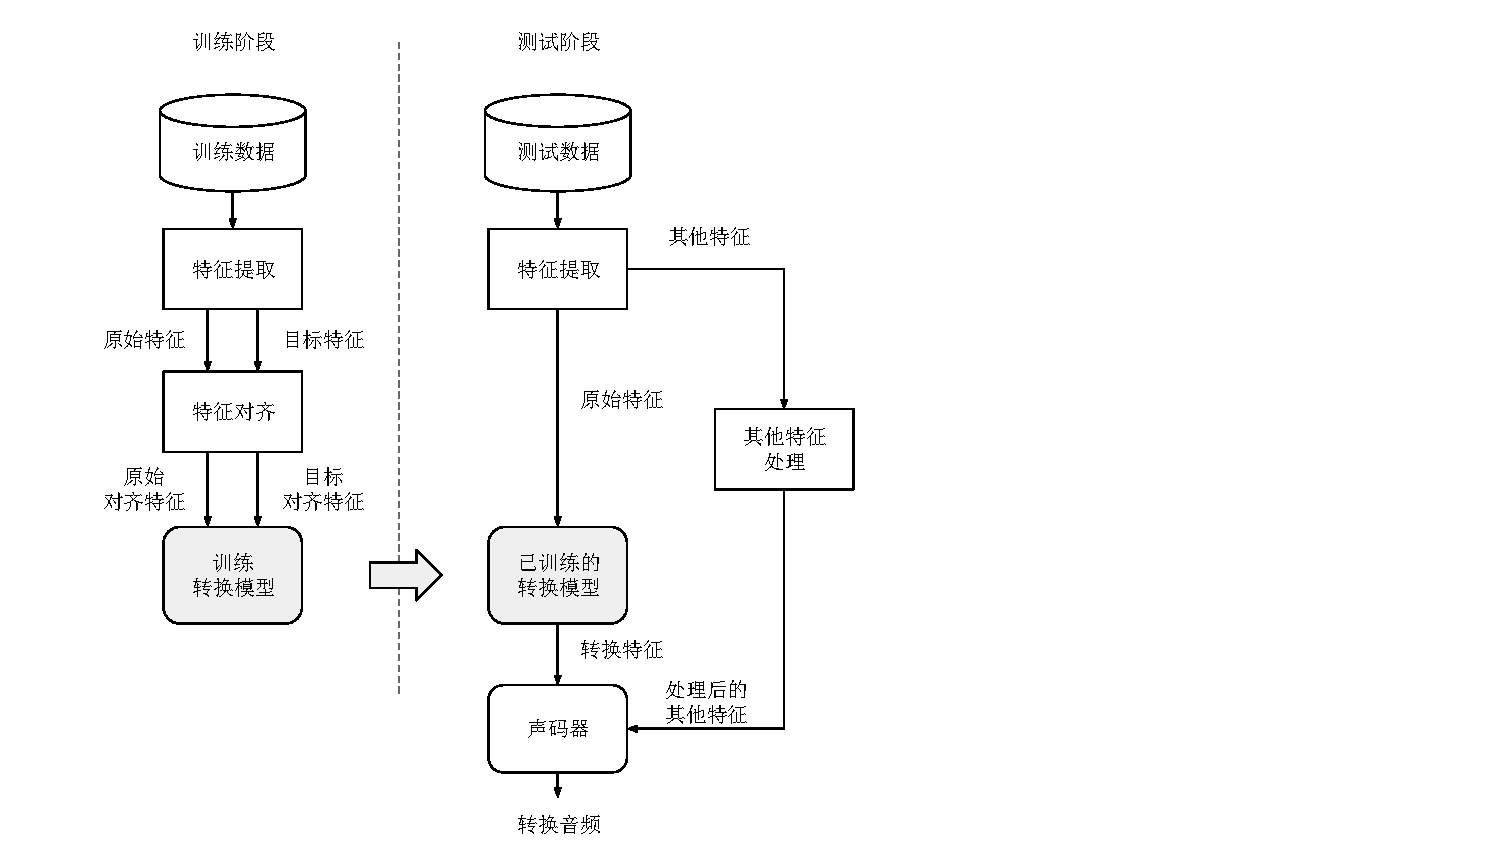
\includegraphics[width=10cm,trim=50 0 310 0,clip]{figure/2_vc_basis.pdf}
    \bicaption[语音转换系统示意图]
    {语音转换系统示意图}
    {Schematic diagram of the voice conversion system}
    \label{fig:vc_basis}
\end{figure}

如图~\ref{fig:vc_basis}所示,语音转换系统通常包含训练模块和测试模块。在训练阶段,首先需要从训练数据中
提取声学特征,通常使用传统的数字信号声码器实现该部分;之后将提取出的原始和目标声学特征进行对齐,对齐算法
取决于使用的语音转换方法,有些转换方法也会省略掉对齐步骤;对齐后的特征会放入转换模型中根据具体的方法进行训练。在测试阶段,测试数据中只有
原始说话人的数据,首先用声码器提取声学特征;然后将特征输入已经训练完成的转换模型中得到转换特征;通常声码器
分析出的特征不只一种,有些方法只会转换一部分声学特征,剩下的其他特征需要做其他处理,如线性变换,保持不变等;
最后将处理后长度相等的声学特征放入声码器中,得到转换音频。

可以看出,决定语音转换系统性能的主要因素为语音分析和合成方法,特征对齐和转换模型。目前的神经网络声码器已经可以稳定地从
真实音频分析的特征中生成非常自然的声音了,因此只要转换模型转换出来的特征足够接近真实,那么声码器就可以等价地生成接近真实的语音。
特征对齐对语音转换的性能有着较大的影响,对于序列层面的对齐而言,受到说话人语速、韵律的影响,长度不同的两段特征往往很难做到精准的对齐,
错误的对齐则会导致向训练数据数据引入错误的标签。因此,近两年提出了很多绕开特征对齐的语音转换方法。转换模型是语音转换中非常重要
的一步,除了能够进可能地转换说话人信息之外,现有的转换模型大多只考虑对说话人信息进行转换,对于韵律特征(如基频,时长)则依旧采用简单的线性变换,
这种变换可以得到不错的效果,但很难真实反应目标说话人的韵律变化,因此较为复杂的韵律转换方法也成为语音转换的目标之一。

评价一个语音转换系统的好坏主要根据该系统所转换的语音来判断,一般分为客观指标和主观指标。
客观指标一般采用梅尔倒谱失真(Mel-cepstral Distortion,MCD)或对数谱失真(Log-Spectral Distortion, LSD),
梅尔倒谱失真计算方法如下,

$$MCD(a^{cvt}, a^{tgt})=\frac{10\sqrt{2}}{ln10T}\sum^{T-1}_{t=0}\sqrt{\sum^{D}_{d=s}(a^{cvt}_{d}(t)-a^{tgt}_{d}(t))^2}$$

其中$a^{cvt}$和$a^{tgt}$分别代表转换特征序列和目标特征序列,$T$和$D$分别代表时间维度和特征维度的大小。梅尔倒谱失真
的计算方法也可以应用到其他特征的失真计算中,如梅尔频谱失真,失真度越小,系统的性能就越好。客观指标可以一定程度上反应转换特征和真实特征之间的差异程度,
但由于语音的质量通常由很多复杂的因素决定,客观指标的计算往往不能充分反应音质的好坏。对于语音生成任务而言,
语音的最终接收者是人,因此最能反应生成语音好坏的方法就是主观评价。主观评价测试可以分为主观意见分测试(Mean Opinion Score, MOS)和对比测试(ABX test)。
主观评价测试一般由测试人员对音频做出1到5分的打分,相似度则需要测试人员在候选音频中选择自己更为偏好的一个。
通过若干名客观的测试人员对测试音频的两个方面进行打分,分别为自然度和相似度。自然度表示语音是否像是人类发出的声音,具体
体现在语音的连贯性,噪音以及音调上。相似度表示语音中的说话人是否像是目标说话人的声音,具体体现在语音的音色上,韵律对相似度也有一定的影响。


\section{语音分析和合成方法}
音频的数字形式可以看成一段长度较长的实数序列,序列的长度由音频时长和采样率决定。例如对于16k采样率的一秒时长的音频,
则可以表示为一个长度为16000的向量,直接对音频样本点序列进行建模目前还有比较大的难度。因此通常会基于语音的短时平稳的特性,
对样本点序列进行分窗成帧,由于每一窗内的信号可以认为是平稳的,则可以对窗内的信号进行分析提取特征,这样可以大大缩短音频表示的序列长度。
因此作为语音转换的主要对象,声学特征的分析对转换模型的建模复杂度和声码器的合成音质都有非常直接的影响。常见的声学特征及其特性如表~\ref{tab:vc_feats}所示\cite{Nurminen2012Voice}。

\begin{table}[!hpt]
    \caption[常用语音转换声学特征示例]{常用语音转换声学特征示例}
    \label{tab:vc_feats}
    \centering
    \begin{tabular}{p{0.3\columnwidth}p{0.6\columnwidth}} 
        \toprule
        声学特征 & 注释 \\
        \midrule
        线谱信号频率(LSF) & 提供稳定,良好的插值性;与共振峰相关性强;对频谱峰建模 \\
        梅尔频率倒谱系数(MFCCs) & 对频谱峰和频谱谷建模;由于对声学距离度量的可靠性,对特征对齐十分有用 \\
        梅尔倒谱系数(MCCs) & 是语音转换和基于HMM的语音合成技术中最常用的频谱表示特征之一。在特征对齐上和MFCCs类似 \\
        共振峰(Formants) & 共振峰的带宽,位置和强度将会是语音转换中非常有用的特征,但是它们的有效估计仍具有挑战性 \\
        频谱采样点 & 频域的采样点也可以被用作语音转换的特征;一般多用于基于频率弯折的方法中。\\
        \midrule
        基频($F_0$) & 基频和对数基频一般通过均值方差的变换转换到目标说话人 \\
        \midrule
        发音标志(Voicing) & 通常二值的发音或非周期信息 \\
        \midrule
        激励频谱 & 有时激励频谱的细节也需要被建模,一般在使用正弦模型是会被用到。\\
        \bottomrule
    \end{tabular}
\end{table}

对于语音的合成方法,可以通过数字信号声码器和神经网络声码器来实现。数字信号声码器通过信号处理的手段
从特征合成音频,主要包括STRAIGHT声码器,WORLD声码器和GL算法;神经网络声码器则是通过神经网络
从大量音频数据中学习特征与音频样本点之间的关系,包括WaveNet, WaveRNN, LPCNet等。
下文将详细介绍源滤波器模型和几种常用的数字信号声码器和神经网络声码器。

\subsection{源滤波器模型}
源滤波器模型是发声理论中非常著名的模型。在源滤波器模型看来,人类的发声过程主要由声道系统完成,
可以分为两个阶段:激励和滤波。其中源激励由喉中的声带产生,滤波由声道的谐振特性完成。
对于元音而言,声源是由声带周期性震动产生的一定频率的声门声音,声源决定元音的音调和音质,
之后由声道和口腔的谐振特性对输入声源进行滤波,得到了不同的元音发音。对于辅音而言,声源主要由
气流在声带,咽部等经过时发出的非周期信号组成,滤波部分同元音类似。声源并不是单一的,实际产生
的声音中往往包含一个或多个声源。发声是一个动态的过程,当声道配置出现改变时,
其谐振特性也会出现改变,随之改变音质和输出的声音。

\begin{figure}[!htp]
    \centering
    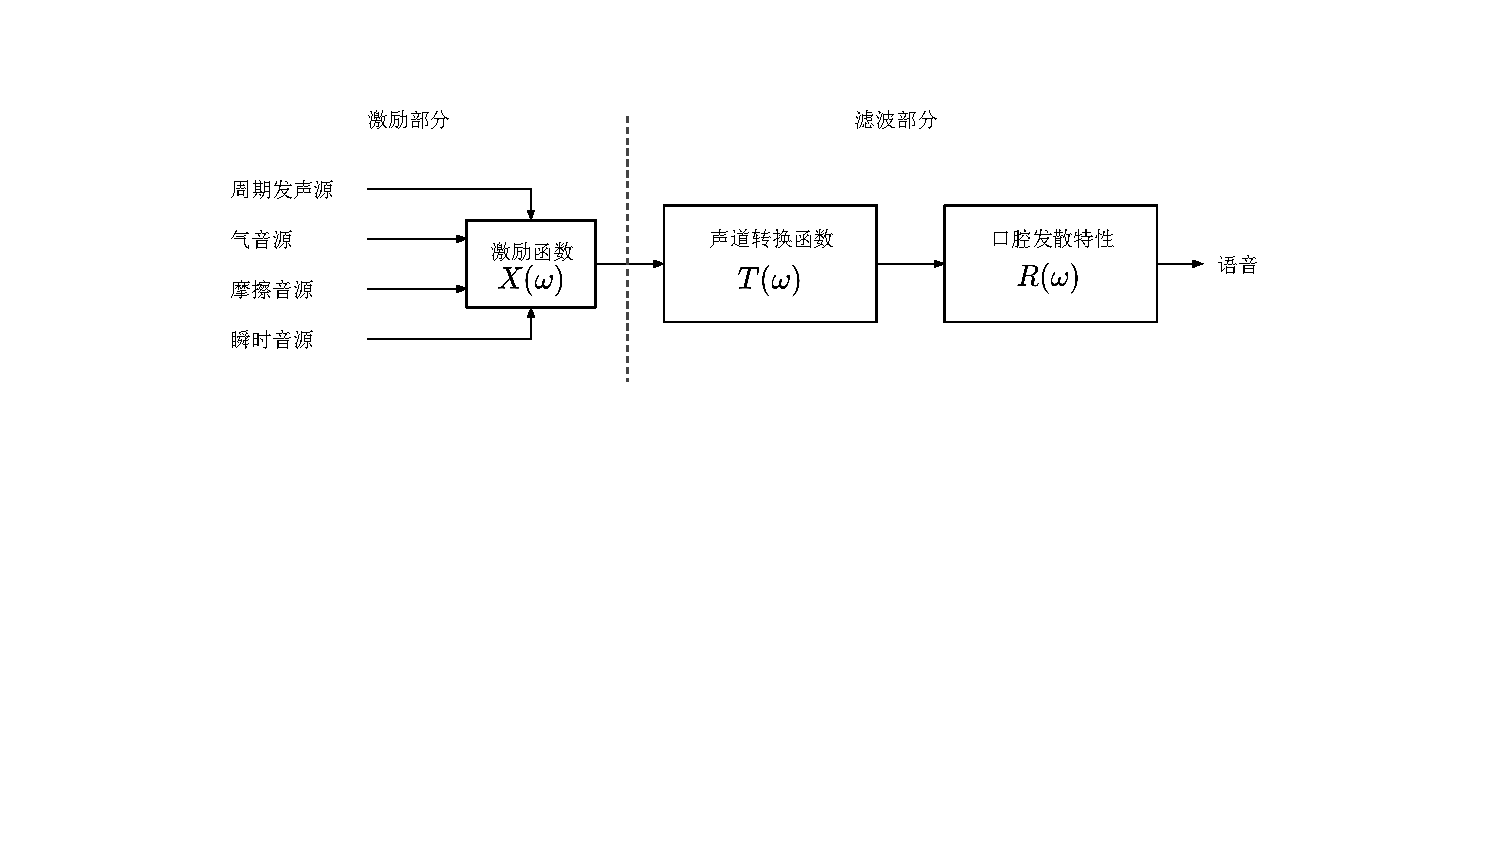
\includegraphics[width=13cm,trim=100 210 100 40,clip]{figure/2_sourcefilter.pdf}
    \bicaption[源滤波器模型示意图]
    {源滤波器模型示意图}
    {Schematic diagram of the source filter model}
    \label{fig:sourcefilter}
\end{figure}

图~\ref{fig:sourcefilter}是源滤波器模型的示意图。不管是元音还是辅音,都会涉及到四种声源:声门周期震动时产生的带有基频的发声源,当空气快速通过
开放不震动的声门时产生的气音源,当空气快速通过狭窄的咽部时摩擦产生的摩擦音源,口腔中压力突然改变而
产生的瞬时音源。其中发声源属于周期信号源,气音源、摩擦音源和瞬时音源属于非周期信号源。
当人类产生声音时,一种或多种音源的组合会作为输入传递给声道滤波,所发出的元音或辅音则可以看做
滤波的输出。

如果声道的配置不发生改变,声道滤波部分就会变成一个线性时不变系统(LTI),同时输出信号$y(t)$
可以由输入信号$x(t)$和系统的冲激响应$h(t)$的卷积来表示,也就是
\begin{equation}
    y(t) = h(t) * x(t)
\end{equation}
转换成频域表达就是
\begin{equation}
    Y(\omega) = H(\omega) X(\omega)
\end{equation}
也就是说,语音谱$Y(\omega)$是由源谱$X(\omega)$和声道滤波谱$H(\omega)$的乘积建模而成。
严格来讲,声道滤波谱$H(\omega)$可以被进一步拆分为声道转换函数$T(\omega)$和口腔的发散特性$R(\omega)$
的乘积,即
\begin{equation}
    Y(\omega) = [T(\omega)R(\omega)]X(\omega)
\end{equation}

源滤波器模型对声音的产生给出了很好的解释和模拟,但也存在较多缺陷。一方面是声源信号的实际处理过程涉及
到更多复杂的非线性变换,直接的线性操作很难模拟真实语音,同时语音的产生是一个时变的过程,声道的配置
根据实际情况不断变化,这些变化的建模也是语音发声的难点之一。但由于源滤波器模型的有效性,其仍受到了
广泛的使用。


\subsection{数字信号声码器}
数字信号声码器是指利用信号处理技术对音频进行特征分析和重建的一系列技术。由于其通常包含了从语音提取特征和
从特征合成语音的一系列功能,从而是语音转换和语音合成等语音生成任务中使用最广泛的一类声码器。接下来将介绍
常用的两个数字信号声码器:STRAIGHT,WORLD,Griffin Lim。

\begin{itemize}
    \item \textbf{STRAIGHT:}全称为自适应内插加权谱的语音转换与重构模型(Speech Transformation
    and Representation using Adaptive Interpolation of weiGHTed spectrum),于1997年提出\cite{kawahara1997speech}。

    \begin{figure}[!htp]
        \centering
        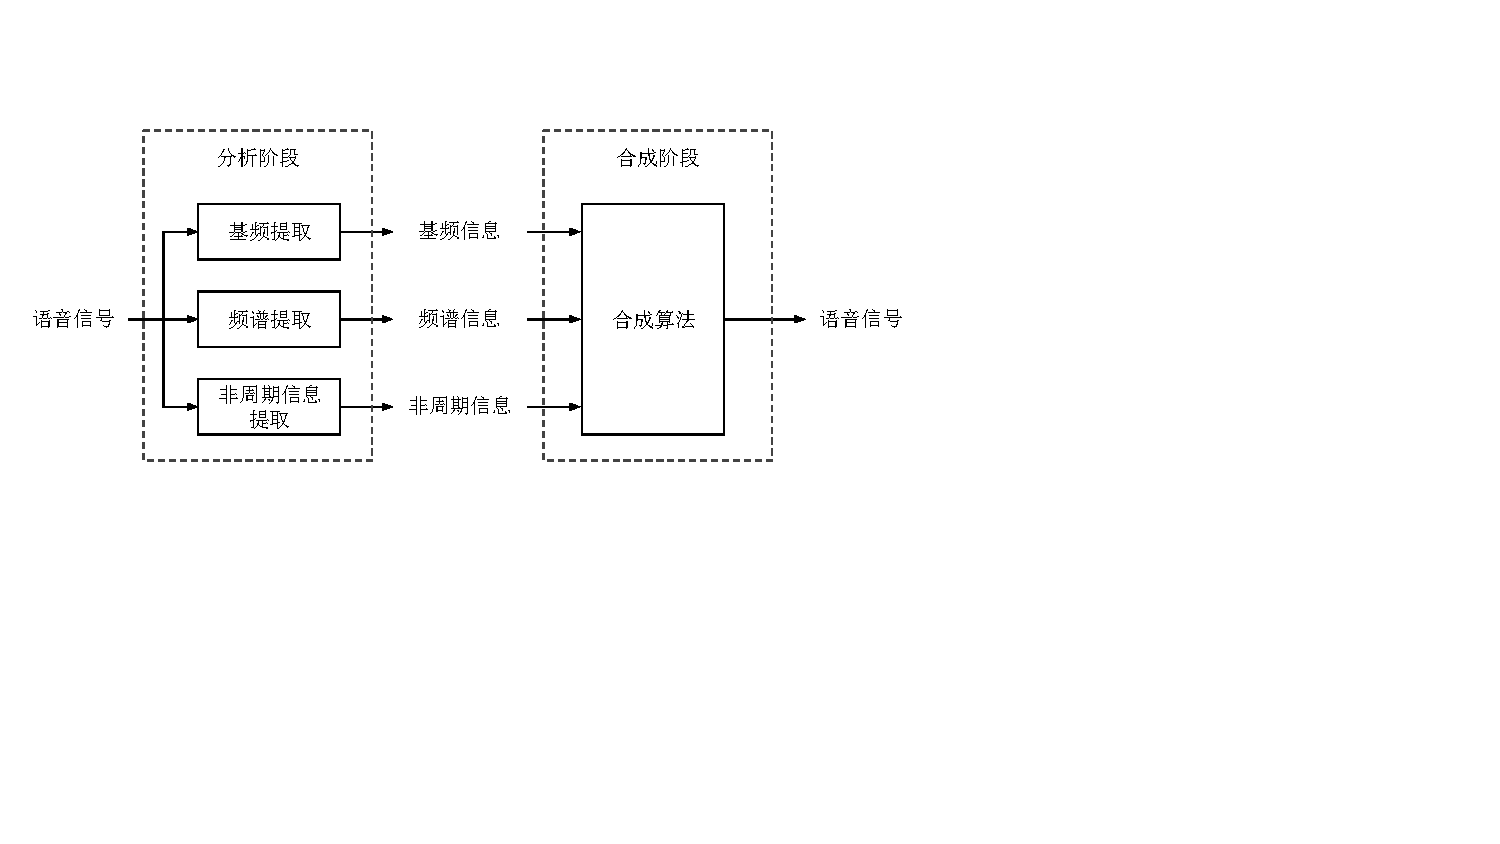
\includegraphics[width=13cm,trim=10 160 260 40,clip]{figure/2_vocoder.pdf}
        \bicaption[STRAIGHT声码器模型框架]
        {STRAIGHT声码器模型框架}
        {Framework of the STRAIGHT vocoder}
        \label{fig:vocoder}
    \end{figure}

    STRAIGHT建立在源滤波器理论上。如图~\ref{fig:vocoder}所示,STRAIGHT通过语音分析从语音信号中提取出三个独立性较强的特征:基频,幅度谱和
    非周期信息。其中基频代表上文中激励部分的频率,也代表语音中的音调高低频率;幅度谱代表语音的在各个频率
    上的福值,可以看成滤波部分中的滤波器分量,决定语音的发音;非周期信息则描述了周期信号和非周期信号之间
    的比例关系,对语音的自然度有很大的作用。STRAIGHT在传统源滤波器信道声码器(VOCODER)的基础上,通过
    在时频域对功率谱进行谱补偿的平滑处理,并在时间轴和频率轴上采样,消除自然语音中周期性的方法来提高语
    谱估计的准确度,进而提升重构语音的音质\cite{杨骋基于简化}。STRAIGHT是传统语音生成任务中最常用的声码器之一。
    \item \textbf{WORLD:}WORLD于2016年作为能够实现高质量实时合成的声码器被提出,由于其在不降低音质的
    情况下高效的合成速度和免费开源的特性,很快就吸引了大量研究者的使用\cite{morise2016world}。与STRAIGHT类似,WORLD也是基于
    源滤波器模型。在WORLD中,首先基频轨迹使用DIO基频提取算法从音频中估计;然后用CheapTrick算法分析频谱,
    分析频谱时不光需要原始音频,也需要上一步提取的基频;最后用PLATINUM算法从原始音频、基频和频谱中估计
    非周期信息。其中WORLD中的非周期信息定义与STRAIGHT中略有不同,STRAIGHT中非周期信息是指非周期信号
    与周期信号之间的比例,而WORLD中则是直接将激励信号作为非周期信息。在合成部分,声带振动是在最小相位
    响应的卷积基和提取的激励信号上计算的,相比STRAIGHT,卷积计算量更小,使得合成速度也会更快。
    \item \textbf{Griffin Lim:}Griffin Lim(GL)于1984年作为一种信号重建算法被提出\cite{griffin1984signal}。
    它可以实现从信号的短时傅里叶变换中估计信号。GL算法的优点是可以直接从频谱构建音频,而不需要预先知道
    相位信息,相位信息由算法估计。缺点是相位的估计依旧不够精准,合成的声音依旧有较为明显的相位不准的情况。
    GL算法首先初始化相位,然后通过不断的计算逆傅里叶变换和傅里叶变换来估计相位信息,一般50次迭代就可以得到
    效果不错的音频。但由于算法本质上是一种迭代算法,因此很难做到实时。
\end{itemize}

目前的数字信号声码器在语音合成的鲁棒性和特征可修改性上都有较好的表现,如STRAIGHT可以实现对音调、声道长度和语速等特性进行600\%
的修改而不会导致音质的明显下降。同时WORLD在处理速度和实时性上也有较好的表现。但当前数字信号声码器所存在的普遍问题
是合成音质与真实音频还有着较大的差距,主要体现在STRAIGHT和WORLD通常会有较为明显的蜂鸣声,由于基频预测不准确
造成的额外噪音,以及人声的不自然。这些一部分是因为数字信号声码器的实现主要是基于信号处理领域的先验知识,声码器和
现实生活中的真实语音并不存在信息交互,由于语音中实际存在大量的复杂信息,仅通过源滤波器模型来模拟语音生成过程是不足以良好的重建语音的。
因此基于深度学习的声码器逐渐被提出,其通过学习大量真实数据,使得语音合成的自然度有了飞跃性的提升。

\subsection{神经网络声码器}
神经网络声码器是指通过神经网络强大的非线性建模能力,来实现从声学特征到音频的合成技术。不同于数字信号声码器,
神经网络声码器通常需要大量的真实音频数据对合成模型进行训练。本文主要介绍两种神经网络声码器:WaveNet和LPCNet。

\begin{itemize}
    \item \textbf{WaveNet:}WaveNet于2016年由谷歌首次提出,最初是作为音频生成模型来实现自然音频的生成\cite{oord2016wavenet}。
    并将其在语音生成,文本转语音,音乐生成和语音识别任务上进行了初步尝试,并在2017年被成功应用到声码器上\cite{tamamori2017speaker}。
    
    \begin{figure}[!htp]
        \centering
        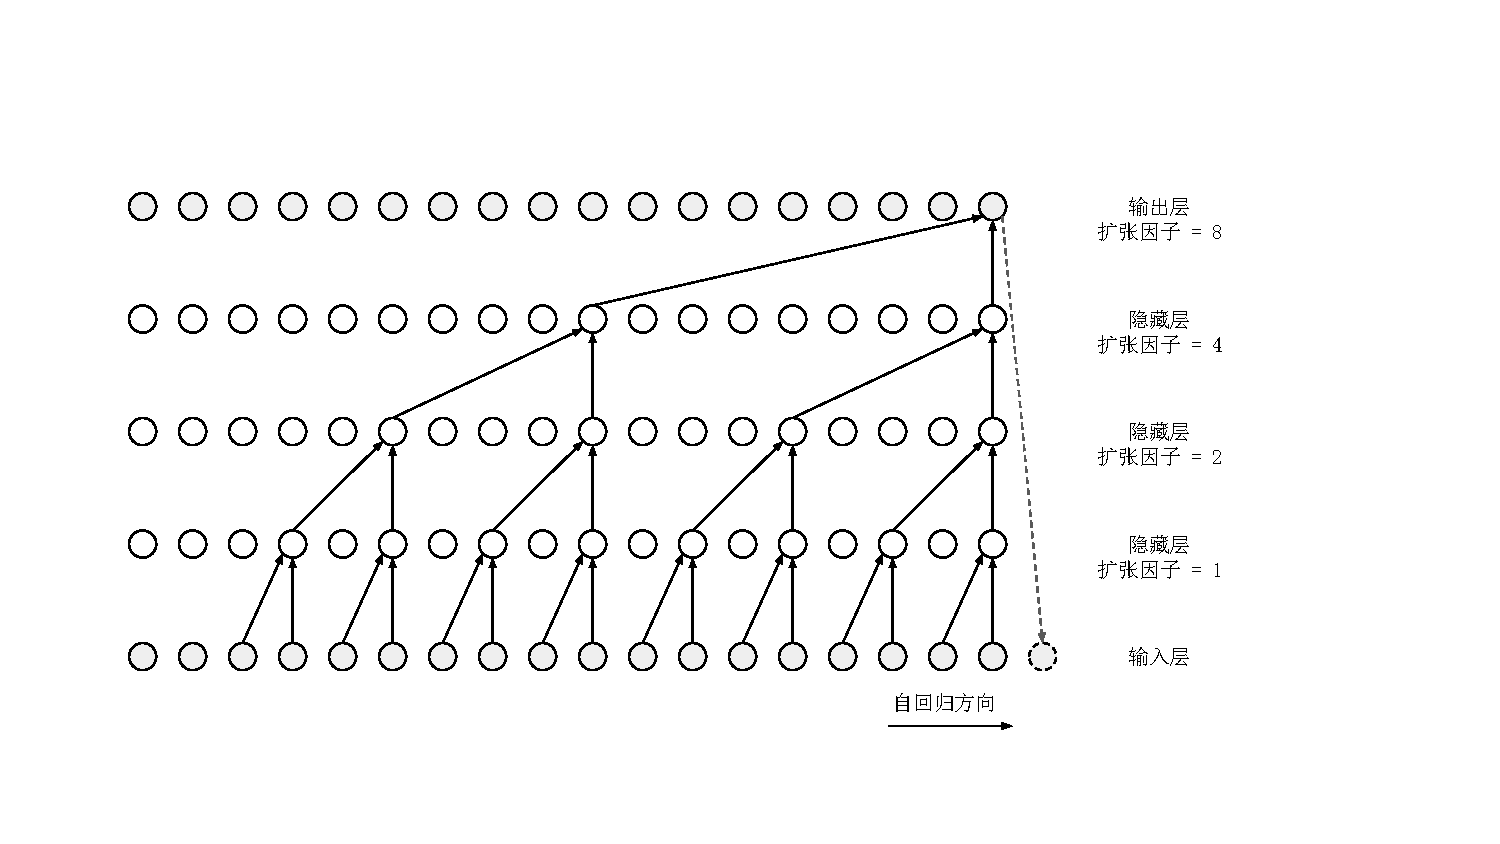
\includegraphics[width=13cm,trim=30 50 130 80,clip]{figure/2_wavenet.pdf}
        \bicaption[WaveNet自回归示意图]
        {WaveNet自回归示意图}
        {Schematic diagram of the autoregressive WaveNet}
        \label{fig:wavenet}
    \end{figure}

    如图~\ref{fig:wavenet}所示,WaveNet是一种自回归模型,即当前时刻的输出取决于之前历史的输出。
    每一个时刻模型会通过音频历史的样本点来预测当前的样本点。由于音频的样本点非常密集,一秒种的音频
    就有上万个样本点,这对自回归模型而言建模难度非常大,因此WaveNet提出使用扩张的因果卷积来增加
    模型的感受域。因果是指模型只会将历史样本点作为输入,预测当前样本点;扩张是指模型会在每层将相隔
    一定距离的样本点作为输入,而不是将所有样本点作为输入。例如图~\ref{fig:wavenet}中隐藏层从低到高
    扩张因子分别为1,2,4,8,即为2的n次方,这样可以使得每一层只有两个输入的情况下,只用4个隐层便
    达到16的感受域。

    WaveNet也可以通过在每一层添加额外的输入来实现在音频生成的过程中加入条件向量,该条件向量即可以是句子级别
    的,也可以是帧级别的,分别对应全局条件和局部条件。在WaveNet声码器中,条件向量可以是任何声学特征,全局
    向量可以代表说话人,实现多说话人的声码器。WaveNet可以生成非常接近自然的语音,但是其缺点也非常明显,
    WaveNet生成时间较长,很难实现实时生成,因此一些提升WaveNet生成效率的改进也被提出,如Parallel WaveNet\cite{oord2017parallel}。
    
    \item \textbf{LPCNet:}LPCNet于2019年提出,是一种高效且实时的神经网络声码器。
    其以WaveRNN声码器\cite{kalchbrenner2018efficient}为基础,结合了深度学习和数字信号处理,显式
    加入了线性预测系数(Linear Prediction Coefficients, LPC)来降低神经网络建模的复杂度。LPCNet可以
    分为两个子网络,帧级别网络和采样点级别网络,以及一个计算LPC的模块。在生成过程中,
    帧级别网络对输入的每一帧声学特征计算条件向量,LPC模块从声学特征中计算LPC,两个特征在帧内保持不变。
    采样点级别网络根据一帧对应的特征,以自回归的方式预测样本点。相比WaveNet, LPCNet的计算复杂度很低,
    可以高效地实现实时合成。
\end{itemize}

\section{特征对齐}
在实际情况中,两个不同的说话人说同一句话时时间长短往往是不一样的,因此就需要对两段对应的特征序列进行对齐操作,
将它们统一成相同的长度。由于特征对齐的情况大多在平行语料的语音转换中出现,因此本文主要说明平行语料语音转换中
的特征对齐。

\begin{figure}[!htp]
    \centering
    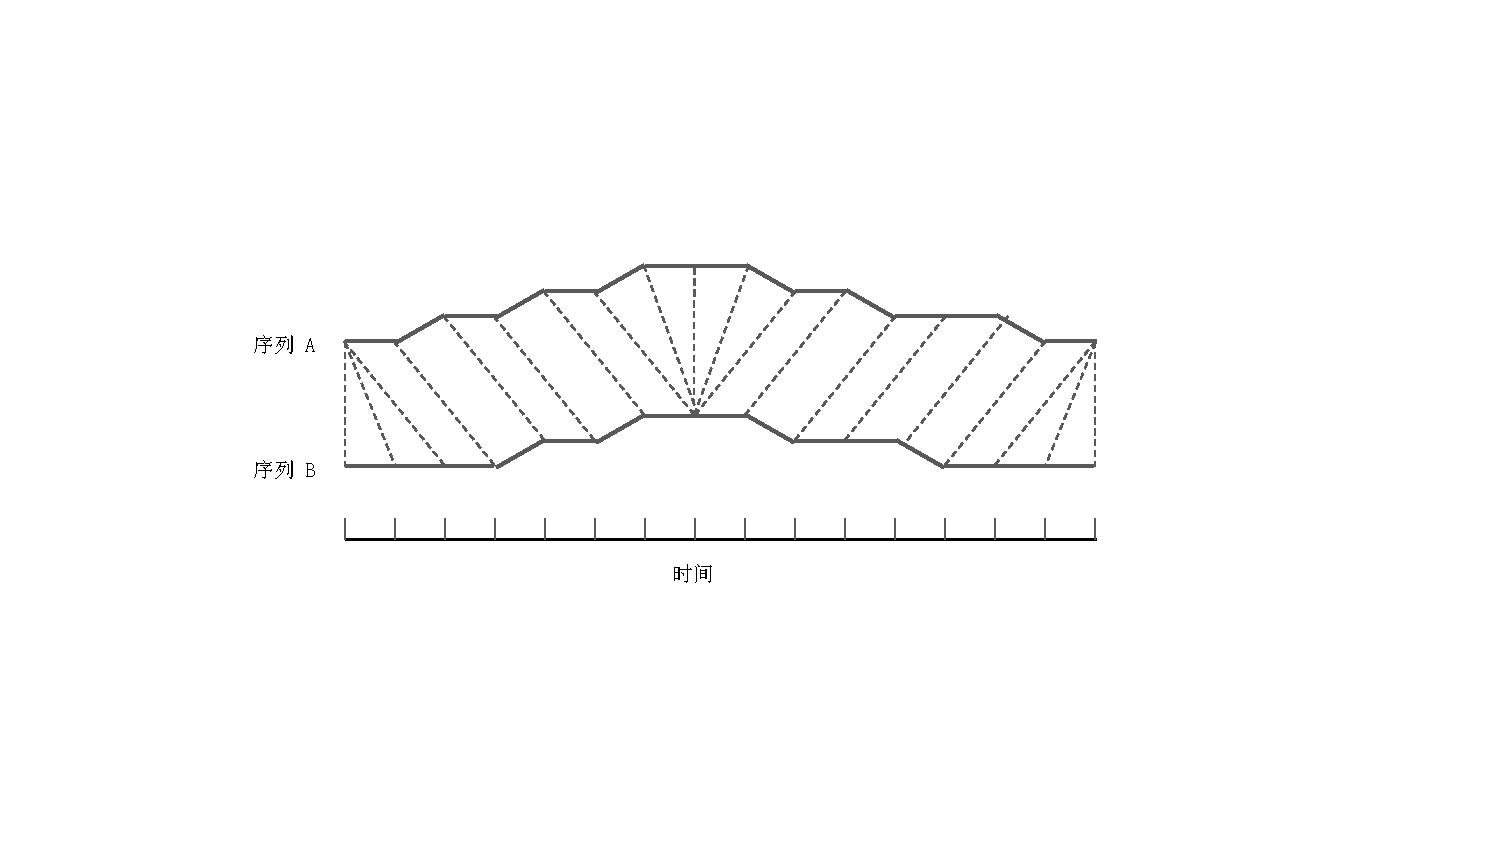
\includegraphics[width=13cm,trim=100 120 150 90,clip]{figure/2_dtw.pdf}
    \bicaption[DTW算法序列对齐示意图]
    {DTW算法序列对齐示意图}
    {Schematic diagram of DTW alignment algorithm}
    \label{fig:dtw}
\end{figure}

对于长度不一致的问题,比较容易想到的方法是通过拉伸的方法将较短的音频拉长到与较长音频长度相同,但是两段语音之间
的长度差距并不是等比例的,即对于内容中的一些字词,原始说话人说的较快,而对于另外一些字词,目标说话人则说的较快。
等比例的拉伸并不能做到较好的帧级别对应。
除此之外,最常用的特征对齐方法就是动态时间规整(Dynamic Time Warpingm, DTW)算法。该算法通过动态规划
来计算两个特征序列之间的最短距离,同时保存该最短距离所对应的路径。如图~\ref{fig:dtw}所示,上下两条粗线为两个特征序列,
中间的虚线代表特征的一一对应关系,对应关系的序列就是两个序列的最短路径。DTW通过计算两个序列之间的最短路径来实现对齐。
然而DTW算法仍有较大的对齐误差,尤其是对于差别较大的特征片段,而较大的对齐误差对转换效果的影响非常大。
因此研究人员将更多的注意力放在了无需对齐的方法上。非平行语音转换方法大多不需要对齐操作,这也是其优势之一。

\section{声学特征转换方法}
声学特征转换是语音转换中最重要的部分,也是当前主要的研究对象。声学特征的转换通常需要一个转换模型来完成,转换模型输入
原始声学特征序列,输出转换后的目标声学特征。本节主要介绍平行语料下的特征转换方法,非平行语料下的特征转换方法将在下一章
中详细介绍。

\subsection{混合高斯模型法}
混合高斯模型法是在深度学习方法之前使用最为广泛的方法之一。该方法使用混合高斯模型(Gaussian Mixture Model, GMM)
对原始说话人声学特征建模,并通过转换函数将原始特征转为对应的目标特征。设原始特征向量为$\mathbf{x}$,用GMM模型表示
其概率分布为
\begin{equation}
    \label{eq:gmm}
    p(\mathbf{x})=\sum^{m}_{i=1}\alpha_iN(\mathbf{x};\bm{\mu}_i,\bm{\Sigma}_i)
\end{equation}

其中$N(\mathbf{x};\bm{\mu},\bm{\Sigma})$代表均值为$\bm{\mu}$,协方差矩阵为$\bm{\Sigma}$的$p$维高斯分布,
可以表示为

\begin{equation}
    N(\mathbf{x};\bm{\mu},\bm{\Sigma})=\frac{1}{(2\pi)^{p/2}}\left| \bm{\Sigma} \right|^{-1/2} exp\left[ -\frac{1}{2}(\mathbf{x}-\bm{\mu})^{T}\bm{\Sigma}^{-1}(\mathbf{x}-\bm{\mu}) \right]
\end{equation}

公式中$\alpha_i$是归一化的正标量权重($\sum^{m}_{i=1}\alpha_i=1$ and $\alpha_i \ge 0$)。在GMM的语音转换
方法中,一个基本假设是声学特征的向量之间是相互独立的,即$t$时刻的目标特征向量$\mathbf{y}_t$只依赖与同一时刻的原始特征
向量$\mathbf{x}_t$。而GMM的一个优点是可以在不同的分布分量中进行软分类,在某种程度上,每一个类别可以代表不同的音素,或其他
音素相关的声学分类。给定观测向量$\mathbf{x}$,判断其属于GMM中一个声学类别$\mathcal{C}_i$的条件概率可以表示为

\begin{equation}
    P(\mathcal{C}_i|\mathbf{x})=\frac{\alpha_iN(\mathbf{x};\bm{\mu}_i,\bm{\Sigma}_i)}{\sum^m_{j=1}N(\mathbf{x};\bm{\mu}_j,\bm{\Sigma}_j)}
\end{equation}

GMM的参数可以通过期望最大化(Expectation-Maximization, EM)算法来估计。用GMM模型在原始声学特征上建模后,
则需要一个转换函数来将输入的原始特征向量转变为对应的目标特征向量,可以定义转换函数如下

\begin{equation}
    \mathcal{F}(\mathbf{x}_t) = \sum^m_{i=1}P(\mathcal{C}_i|\mathbf{x}_t)\left[ \mathbf{v}_i + \bm{\Gamma}_i \bm{\Sigma}_i^{-1} (\mathbf{x}_t-\bm{\mu}_i) \right]
\end{equation}

转换函数的参数只要是$\mathbf{v}_i$和$\bm{\Gamma}_i$,输入其中$\mathbf{v}_i$表示目标特征的期望均值,$\bm{\Gamma}_i$表示原始特征与目标特征的协方差矩阵。
这些参数通过最小化转换的均方误差来估计。误差可表示为

\begin{equation}
    \epsilon = \sum^n_{t=1} \left| \left| \mathbf{y}_t - \mathcal{F}(\mathbf{x}_t) \right| \right|^2
\end{equation}

该方法可以通过只对原始特征进行GMM建模来实现逐帧的语音转换。在此之后,一些基于GMM对目标特征建模的方法也被提出\cite{kain1998spectral}。
但是混合高斯法建立在不同帧之间相互独立的假设之上,只能实现逐帧转换,这是限制GMM转换性能的一个主要因素。

\subsection{码本映射法}
码本映射法(Codebook Mapping)的历史比混合高斯法更为悠久,是最早出现的语音转换方法之一。直观的码本映射法即是将原始和目标特征合并在一起,
训练一个大的码本。在转换时,原始特征先通过码本得到码本编号,与该编号最接近的目标特征即是转换特征。之后研究人员在码本映射法中加入了矢量量化(Vector Quantization, VQ)
的方法。该方法先对原始和目标特征通过VQ各自生成一个码本。同时对平行特征序列用DTW算法进行对齐,根据特征之间的对应关系生成直方图。对于原始说话人
每个码本向量的直方图,通过加权平均得到该码本向量对应的码本映射。在转换阶段,对原始特征的每一个特征向量,先通过原始说话人的码本编码得到量化向量,
再用该向量对应的码本映射得到转换特征。

码本映射法的基本思想简单直接,但也有比较明显的缺陷。首先逐帧转换对转换语音的连贯性有很大的影响,其次对声学特征离散化表示进行聚类会损失较多的声学信息,导致转换单一,自然度较差,
以及线性平均造成的严重过平滑问题。
对于这些缺陷,研究人员也提出一些改进措施比如码本词的线性加权组合法、分层的码本映射法和局部线性转换法等等。

\subsection{频率弯折法}
频率弯折法与之前介绍的语音转换方法不同,它是基于规则的语音转换方法。频率弯折法一般是通过频域中较为突出的区域特征来建立
原始与目标的映射关系(如共振峰的中心频率)。比较典型的频率弯折法是基于声道长度归一化(Vocal Tract Length Normalization, VTLN)的语音转换方法。

在基于VTLN的方法中,最优频率弯折函数$\mathcal{w}(\mathcal{f}, \theta)$的参数可以定义为

\begin{equation}
    \theta = \mathop{\arg\min}_{\theta}\int^{\pi}_{\mathcal{w}=0}\left| Y(\mathcal{f})-X(\mathcal{w}(\mathcal{f},\theta)) \right|^2 d\mathcal{w}
\end{equation}

其中$X(\mathcal{f})$和$Y(\mathcal{f})$分别代表原始和目标频谱。一般频谱弯折函数中只有一个参数$\theta$,
常见的弯折函数有二次函数

\begin{equation}
    \mathcal{w}_{\theta}(\mathcal{f}) = \mathcal{f} + \theta\left[ \frac{\mathcal{f}}{\pi}-(\frac{\mathcal{w}}{\pi})^2 \right]  
\end{equation}

以及双线性函数

\begin{equation}
    \mathcal{w}_{\theta}(\mathcal{f}) = \frac{\mathcal{f}-\alpha}{1-\alpha \mathcal{f}}
\end{equation}

频率弯折法通过对频谱中最显著的部分进行连续函数变换来实现语音转换,这样做的好处是可以在保留频谱中的大部分信息的前提下,
保证频谱的连贯性。因此频率弯折法往往可以得到比较好的音质,但是由于频谱中的说话人信息并不只包含在最显著的特征中,同时也存在于其他特征上(如共振峰带宽)。
因此频率弯折法的主要缺陷在于转换音频的说话人相似度较低。

\subsection{神经网络法}
神经网络(Neural Networks, NN)是一种从生物学中受到启发的建模方式。神经网络的发展历史较早,但早期多专注于理论阶段和复杂度相对较小的模型实验,
因此也提出了很多模型结构但难以验证。
随着大数据和计算机硬件的飞速发展,神经网络模型的参数量可以随着训练数据量的增多和计算速度的变快而不断地增加,从而可以实现更为复杂的
网络结构和建模任务,我们称之为深度学习。由于神经网络具有强大的建模能力,使得其在很多建模任务上相较传统的机器学习算法都取得了突破性的进展。如今,神经网络
已经在很多领域得到了广泛的应用,如计算机视觉,自然语言处理和智能语音等。

\begin{figure}[!htp]
    \centering
    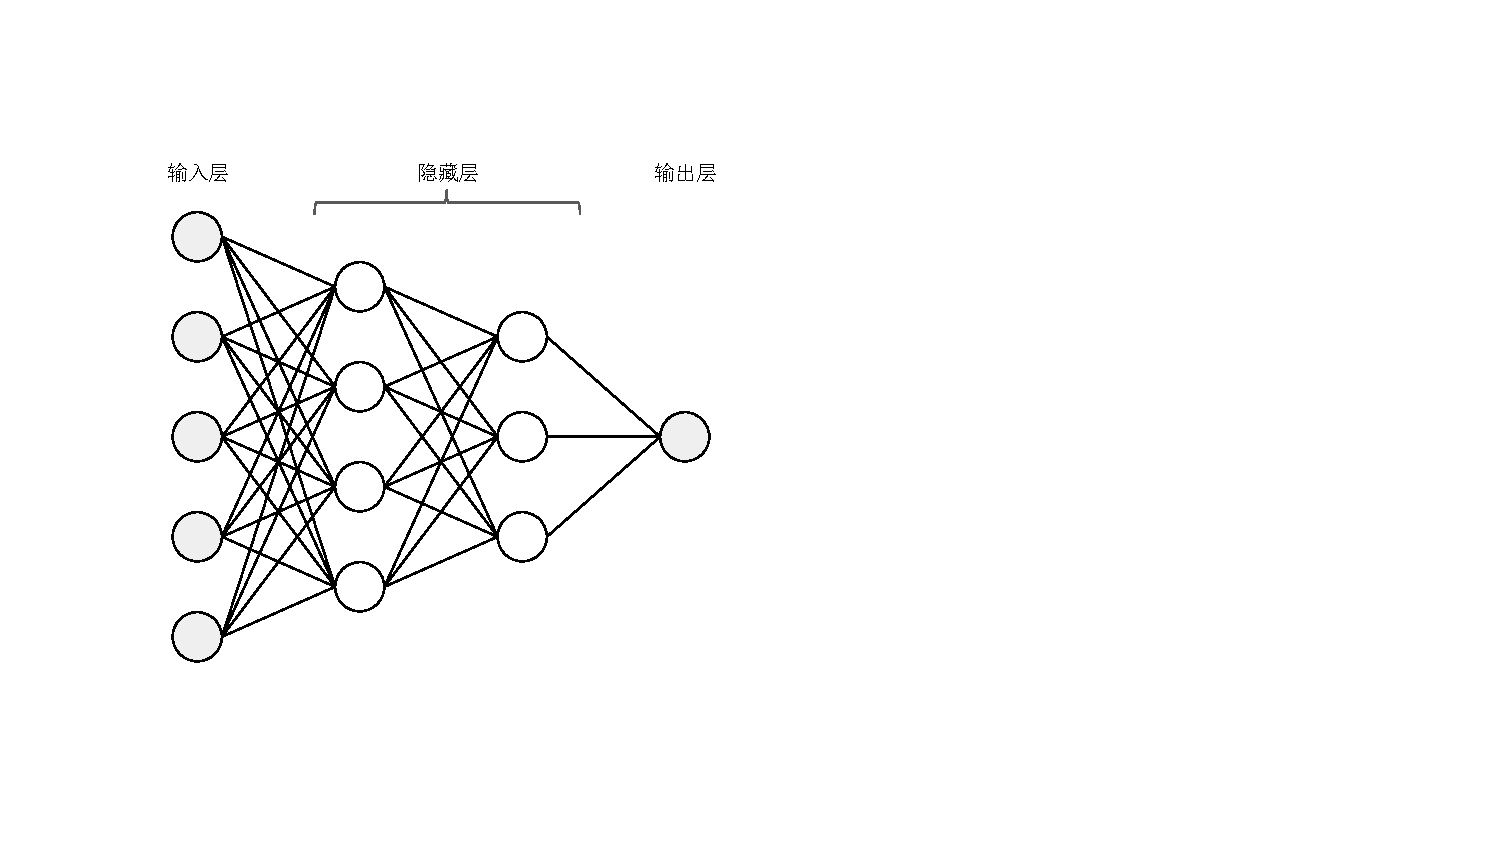
\includegraphics[width=10cm,trim=50 70 330 50,clip]{figure/2_mlp.pdf}
    \bicaption[多层感知机结构图]
    {多层感知机结构图}
    {Architecture of the Multilayer Perceptrons}
    \label{fig:mlp}
\end{figure}

最初的神经网络由多层感知机发展而来(Multi-Layer Perceptrons, MLP)。如图~\ref{fig:mlp},MLP由一个输入层,多个隐藏层,一个输出层组成。每一层都
包含有多个神经元,每个神经元都可以对输入做加权线性变换,并将结果输出。经过逐层的前向传播,MLP在输出层输出模型结果。在训练时,
MLP的输出会根据对应的标签计算误差,并使用反向传播(Back Propagation, BP)算法计算梯度,并根据每个参数的梯度更新模型。
从而使得模型可以不断的拟合训练数据。在数据量较大的情况下,神经网络具有较强的泛化能力,在测试集上的性能往往要好于传统方法。
在深度学习时代,神经网络的种类层出不穷,其中较为著名的包括深度神经网络(Deep Neural Networks, DNN),循环神经网络(Recurrent Neural Networks, RNN),
卷积神经网络(Convolutional Neural Network, CNN)等,其中每个网络也有较多的变种。

基于人工神经网络(Artificial Neural Networks, ANN)的语音转换方法在2009年被提出\cite{desai2009voice}。
作者用4层的神经网络学习原始特征到目标特征的映射关系,相邻两层之间采用全连接的形式。
在训练阶段,首先从原始和目标音频中分析,25维的梅尔倒谱系数和1维基频特征;然后用DTW算法对平行特征序列进行对齐,模型的输入是原始特征,标签是目标特征;
最后使用反向传播算法对模型进行训练。论文中的实验结果说明了基于神经网络的语音转换方法在主观实验和客观实验上都普遍好于基于GMM模型的语音转换方法。
该工作证实了神经网络在语音转换任务上的可行性。之后针对类ANN网络的语音转换改进方法也不断被提出。

\begin{figure}[!htp]
    \centering
    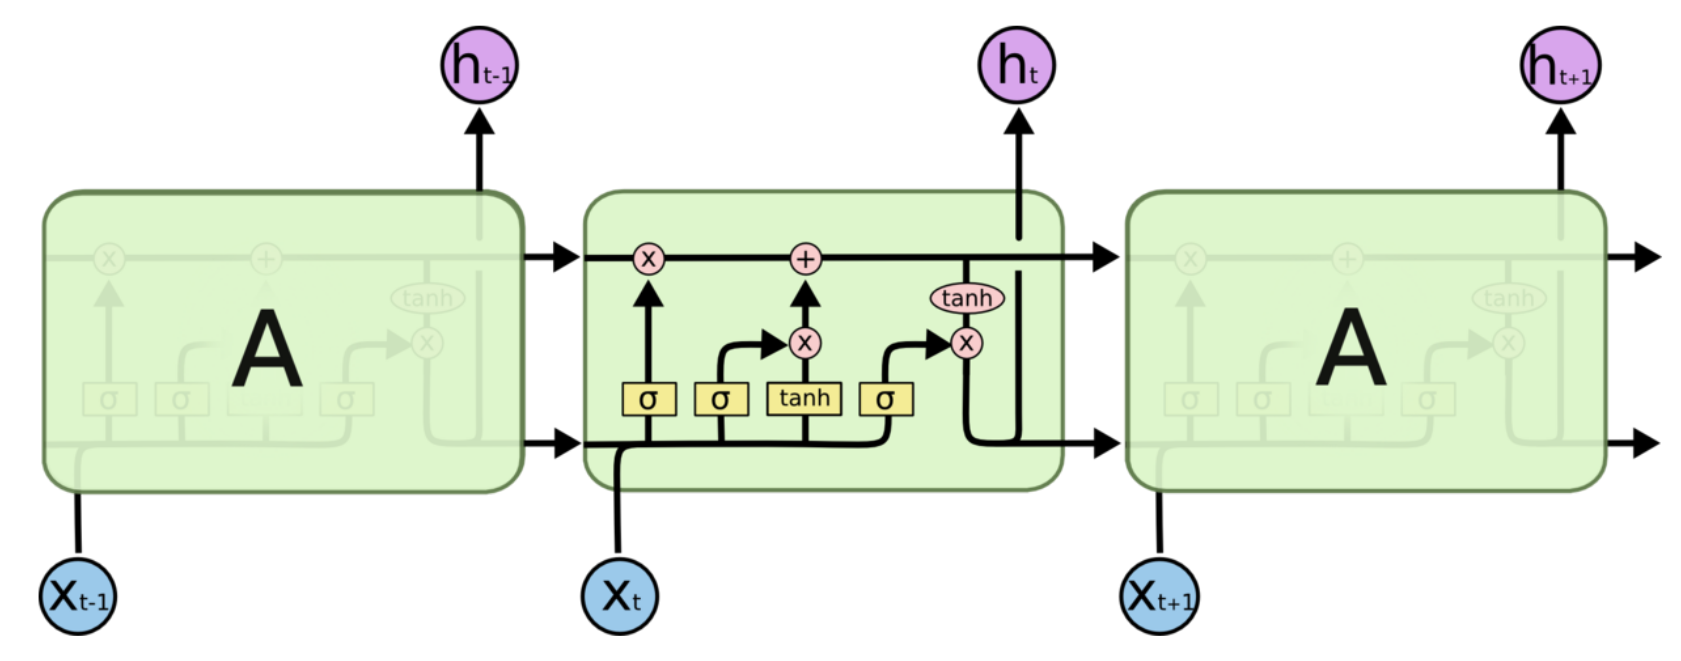
\includegraphics[width=10cm,trim=0 0 0 0,clip]{figure/lstm.png}
    \bicaption[长短时记忆网络结构图]
    {长短时记忆网络结构图}
    {Architecture of the Long Short Term Memory}
    \label{fig:lstm}
\end{figure}

如前文所述,很多方法都存在声学特征帧相互独立的假设,然而这个假设与常识有所矛盾,语音作为一个时序序列,距离越近的时刻往往相关性就越大。即使有些方法
也被提出来弥补这方面的缺陷,如加入动态特征,当前方法仍然没有很好的贴合时间序列的特性来实现更好的转换性能。在2015年,研究人员提出了基于
深度双向长短时记忆网络(Deep Bidirectional Long Short Term memory, DBLSTM)的语音转换方法\cite{sun2015voice}。该方法创新点主要为使用了包含DNN和双向LSTM的
转换模型。LSTM是RNN的一个变种,针对RNN对长时信息的建模能力较差,LSTM在RNN的单元(cell)中加入了三个门控机制,分别为输入门,遗忘门和输出门。
单元的状态值代表历史时刻的信息,其在网络的序列计算中不断更新。
如图~\ref{fig:lstm}所示,三个门控会通过$sigmoid$函数输出0到1之间的值,输入门表示当前时刻输入加入单元状态值的比例,
遗忘门表示当前时刻要从单元状态值中遗忘多少信息,输出门表示从更新后的单元状态值中输出多少比例到下一单元。设输入特征序列
$\mathbf{x}=\left\{x_1,x_2,...,x_T\right\}$,当前隐藏层的激活值为$\mathbf{h}=\left\{h_1,h_2,...,h_T\right\}$,
LSTM单元在$t$时刻的计算过程可以用如下公式表示

\begin{align}
    & i_t = \sigma (W_{i}x_t + U_ih_{t-1}+b_i) \\
    & f_t = \sigma (W_{f}x_t + U_fh_{t-1}+b_f) \\
    & c_t = f_tc_{t-1} + i_ttanh(W_cx_t+U_ch_{t-1}+b_c) \\
    & o_t = \sigma (W_{o}x_t + U_oh_{t-1}+b_o) \\
    & h_t = o_ttanh(c_t)
\end{align}
  
其中$\sigma$表示$sigmoid$激活函数,$W$和$U$为可学习的矩阵参数,$i$,$f$和$o$分别代表输入门,
遗忘门和输出门,$c$表示单元状态。双向网络在单向网络的基础上添加了额外一层,该层以由后向前的时间顺序
传播,两个相反方向的LSTM层输入同一个特征序列,并将输出的隐层序列拼接起来,形成最终的输出。在\cite{sun2015voice}中,
转换模型由6层BLSTM网络组成,并使用基于时间的反向传播算法(Back-Propagation Through Time, BPTT)训练模型。实验表明,
基于DBLSTM的转换模型明显好于基于DNN的方法。对比加入动态特征的DNN方法,DBLSTM模型在平均意见分(Mean Opinion Score, MOS)上
高出0.5分。

上面所述方法都有效促进了语音转换音质的提升,但这些方法都会受到特征对齐准确度的限制。如前文所述,特征对齐的准确度对语音转换有
很大的影响,目前所用到的特征对齐方法普遍还是基于DTW算法,而韵律差别较大的特征序列往往会使DTW算法的准确度急剧下降。
因此,基于序列到序列和注意力机制(Sequence-to-Sequence Attention)的语音转换模型于2019年提出\cite{tanaka2019atts2s}。序列到序列和注意力机制
模型是序列建模中非常著名的模型,它可以实现不受输入长度约束的不定长输出。序列到序列和注意力机制模型通常由三个模块构成:编码器,
注意力模块和解码器。其中编码器对输入的特征序列进行变换,将其转换成相同长度的抽象特征序列;解码器采用自回归的计算方式,输入
上一时刻的输出,和当前时刻注意力机制计算的注意力向量进行拼接,再去预测当前时刻的输出;注意力机制是一种序列相似度的对齐机制,
其输出向量的物理意义是指与当前解码器输入向量(Query, Q)最相似的编码器输入向量(Key, K)的特征值信息(Value, V)。公式表示如下

\begin{equation}
    \mathbf{c}_t = \sum^n_{i=1}\alpha_{t, i}\mathbf{h}_i
\end{equation}

其中$\alpha_{t, i}$表示$t$时刻输入与第$i$个编码器输入向量的匹配程度。$\mathbf{h}_i$代表第$i$个输入向量。
$\alpha$的计算方法如下

\begin{equation}
    \alpha_{t, i} = \frac{exp(score(\mathbf{s}_{t-1},\mathbf{h}_i))}{\sum^{n}_{i^{'}=1}exp(score(\mathbf{s}_{t-1},\mathbf{h}_{i^{'}}))}
\end{equation}

$\mathbf{s}$是指编码器输入向量。$score$的计算方法有很多种,如余弦法,点乘法,基于位置的方法等。
注意力机制在解码器解码时向其提供输入序列的局部信息,以使解码结果与输入的对应位置保持一直,另一方面,
注意力机制可以完成更为复杂的对齐操作,可以实现相比DTW更为准确的对齐路径,从而提升转换性能。除此之外,
论文中也额外添加了一个编码器和一个解码器,通过对原始特征序列和目标特征序列进行重构,来尽可能在转换过程中
保留特征中的语义信息。实验证明,该方法的转换语音在自然度和相似度上都要好于基于GMM的语音转换方法,
另外该方法也好于基于LSTM的语音合成方法。这也是目前在平行语音转换任务上转换音质最好的方法之一。

\section{韵律转换}
韵律一般是指语音的发音节奏,语速和表现力等,与说话人的说话风格有很大的关系,准确的韵律转换可以使
转换语音更接近目标说话人。与韵律相关的特征主要有基频和时长,下面将对这两种特征的主要转换方法做以说明。

\subsection{基频转换}
基频(Fundamental Frequency, F0)代表着语音当中的最低频率,由于基频在人耳的感知中具有最大的响度,
因此基频常与语音的音调等价。基频的转换是十分必要的,尤其对于跨性别语音转换,男性的基频分布与女性的
基频分布往往差别较大,此时基频的转换效果会直接影响转换语音的相似度。

传统的基频转换方法通常使用均值方差归一化的线性转换。该方法非常简单直接,首先从原始和目标训练数据中提取基频序列;
然后分别计算原始基频序列和目标基频序列的均值($\mu_s$, $\mu_t$)和方差($\sigma_s$,$\sigma_t$);在转换阶段,对原始测试基频用原始说话人的均值方差先做归一化,
再用目标说话人的方差均值对其做逆归一化。转换过程可用公式表示如下

\begin{equation}
    F_0^t = (F_0^s - \mu_s)\frac{\sigma_t}{\sigma_s} + \mu_t
\end{equation}

其中$F_0^s$和$F_0^t$分别代表原始基频和转换目标基频。在乐理中,基频在对数域会呈现等差增长,
即音高频率在对数域是平均分布的,且在\cite{erro2009voice}中,基频在对数域比在
线性域能够更好地被正态分布拟合。因此在实际操作中更倾向于以对数基频为线性转换的对象。

然而线性变换也存在明显的缺陷,该方法只能改变基频的分布,而不能改变基频的变化趋势。在\cite{chen2018high}中,
作者在平行语料的语音转换任务中,使用梅尔频谱特征代替传统的数字信号声码器分析特征(梅尔倒谱系数,基频,非周期成分),
直接用转换模型学习梅尔频谱中基频信息的转换。经过实验验证,使用模型学习基频的隐式转换可以获得更接近目标基频轨迹的
转换语音。

\subsection{时长转换}
时长转换的常用方法与基频转换类似,也是使用线性转换的方法改变语速,即对一整句话进行固定比例的拉伸操作来改变时长,如线性插值或样条插值。
除此之外一些基于音素的韵律转换方法也被提出\cite{helander2007novel}。如前文所述,
在\cite{tanaka2019atts2s}中,序列到序列的建模方式可以有效实现不等长序列的映射关系学习,
同时也可以做到不定长序列的生成,该模型的解码器通过在每个时间步判断停止令牌(stop token)来决定
是否需要停止解码。但是,时长转换由于评价指标较难定义,且对说话人相似度的影响较小,目前研究的主要重心仍集中在
频谱转换上。

\section{本章小结} 
本章主要介绍语音转换系统的典型框架及其主要部分,包括语音分析和合成方法,
特征对齐,频谱转换方法和韵律转换方法。本章首先对语音转换系统,评价指标及常用特征进行了回顾;
然后介绍了语音转换系统中每个部分的主流技术及最新进展,并对其优势和不足进行了分析。作为语音转换中
最重要的部分,本文对常见的几种平行语料的频谱转换方法进行了详细的介绍。
\chapter{非平行语料的语音转换}

\section{引言}
上文已经介绍了语音转换的典型框架及其各部分的主要技术,其中对于频谱转换方法主要介绍了平行语料下的
语音转换方法如混合高斯模型法,码本映射法,频率弯折法和神经网络法。随着语音转换技术的不断发展,
目前在平行语料下已经可以得到比较自然的转换声音了,然而在语音转换的实际应用中,平行语料的获取
往往需要搜集大量网络数据并从中匹配原始和目标的平行数据对,甚至原始或目标说话人亲自录制平行语料,
同时还需要尽可能保证训练数据与实际测试数据的环境条件相同,
这些都大大增加了语音转换模型的构造成本。相比平行语料而言,非平行语料的获取成本会低很多,对于知名度较高
的说话人,往往可以搜集到大量非平行语料数据。因此,基于非平行语料的语音转换方法更符合语音转换任务的实际需求。
为了与实际应用相结合,研究人员在近两年提出了许多能够实现非平行语料的频谱转换方法。如今,非平行语料正在成为语音转换的
研究热点和难点。

本章将主要介绍非平行语音转换及当前常见的频谱转换方法,包括基于音素后验概率图的方法,对抗训练法以及变分自编码器法。
之后将重点介绍基于CycleGAN的语音转换方法,该方法是非平行语料的语音转换方法中使用较为广泛的一种,也与本文的研究工作
密切相关。

\section{非平行语料语音转换概述}
非平行语料的语音转换(Non-parallel Voice Conversion)是指在原始和目标说话人的训练数据不包含相同的文本内容的条件下,
构造语音转换模型。在语音分析合成方法和韵律转换方法上,两者没有本质区别。然而不同于平行语料的语音转换,非平行语料的语音转换属于无监督任务,对于原始说话人的每一句话,并不存在对应
的标签,因此模型需要通过额外模型的帮助或特殊的训练方法来实现从两个说话人的特征中学习说话人信息并转换。非平行语料语音转换通常不需要特征对齐的步骤,两者的主要差别在频谱转换方法中。
早期的非平行语料语音转换方法以自适应的方法为主\cite{mouchtaris2004non,lee2006map}。如最早于2004年提出\cite{mouchtaris2004non},
作者在基于GMM的语音转换方法上,先使用已有的说话人平行语料预训练一个转换模型,
然后再将非平行语料的原始和目标说话人分别对转换模型做说话人自适应,从而实现非平行语料的语音转换。
另一种可行的办法是使用语音合成中的单元选择(Unit Selection)技术\cite{sundermann2006text},
从目标特征中选择与原始特征最匹配的特征帧,来实现无监督的语音转换。为了保证声学特征的连续性,当前帧的值由匹配目标帧和上一帧
加权决定。

随着近两年非平行语料的语音转换关注度增加,研究人员基于神经网络技术提出了一些更为有效的解决方案。如音素后验概率图法,
对抗训练法和变分自编码器法。其中,基于循环一致性生成对抗网络(CycleGAN)的语音转换方法在不需要任何额外数据和模型
的前提下,实现了与平行语料转换方法接近的转换性能。下文将详细介绍这些方法。

\section{常见特征转换方法}
\subsection{音素后验概率图法}
音素后验概率图法(Phonetic PosteriorGrams, PPGs)最早于2016年提出,是一种可以实现任意原始说话人到特定目标说话人(Any-to-One)的语音转换方法\cite{sun2016phonetic}。
该方法的核心思想是使用一个说话人无关特征作为中间特征,来作为原始和目标声学特征之间的媒介。通过说话人无关特征的提取器可以从任意原始说话人的语音中提取中间特征,然后只需要训练
一个从说话人无关特征到目标说话人声学特征之间的映射模型便可以实现语音转换。最直观的说话人无关特征即是文本特征,因此文章中使用每一帧对应的音素后验概率图作为中间特征,
并用语音识别系统(Automatic Speech Recognition, ASR)作为该特征的提取器。

\begin{figure}[!htp]
    \centering
    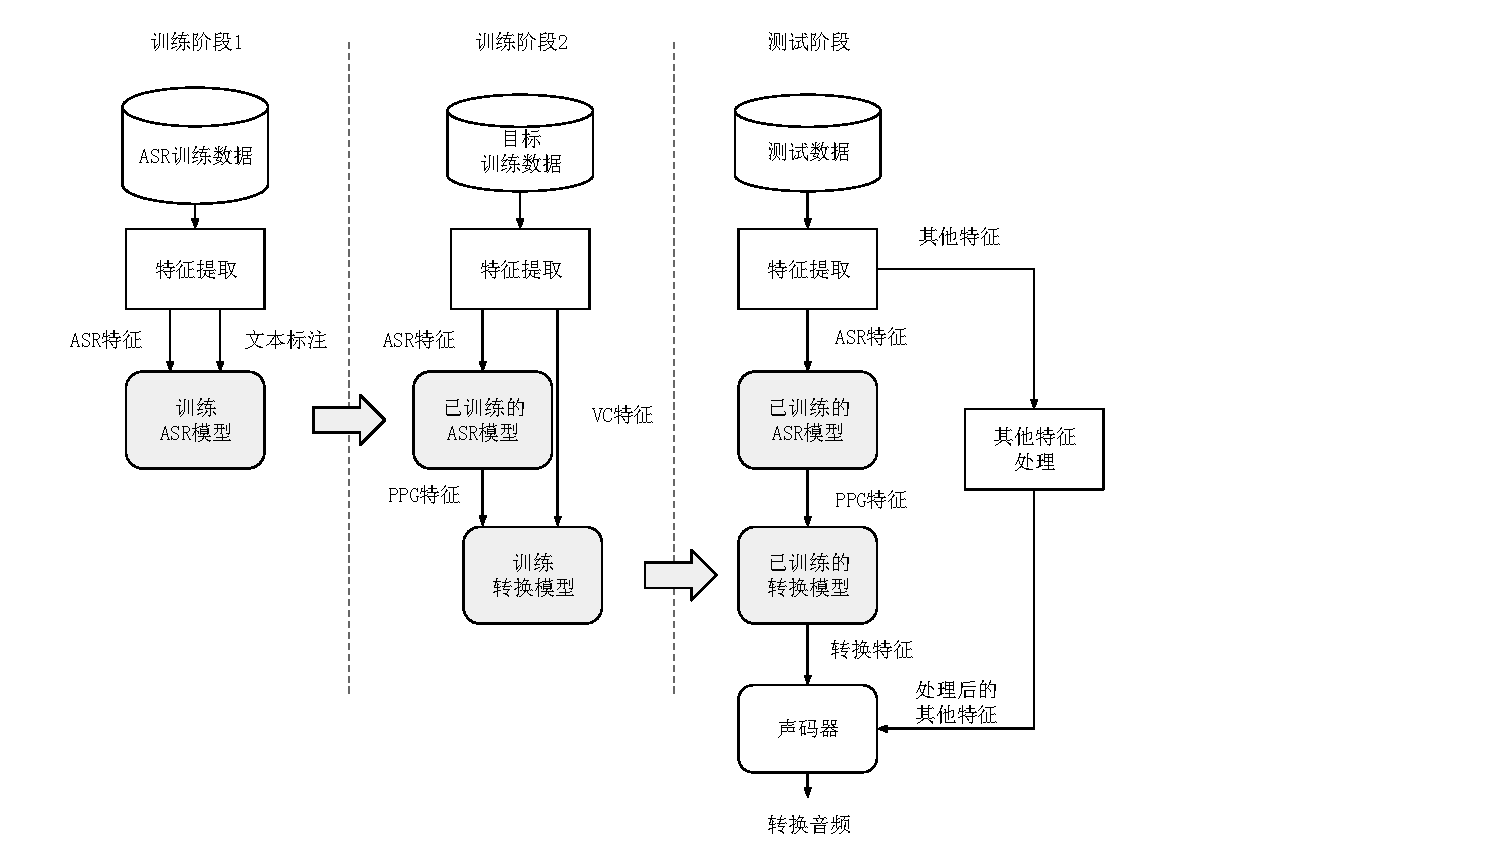
\includegraphics[width=13cm,trim=10 0 160 0,clip]{figure/3_ppg.pdf}
    \bicaption[音素后验概率图语音转换方法示意图]
    {音素后验概率图语音转换方法示意图}
    {Schematic diagram of the Phonetic PosteriorGrams Voice Conversion method}
    \label{fig:ppg}
\end{figure}

如图~\ref{fig:ppg}所示,基于PPG的语音转换方法可以分为三个模块:训练模块一,训练模块二和转换模块。在训练模块一中,使用标准的
语音识别数据集训练说话人无关的语音识别系统,这里需要用到语音识别中的声学特征如梅尔频率倒谱系数(MFCC)或滤波器组(Filter Bank, FBank)。
语音识别模型的训练可以依靠Kaldi开源工具\cite{povey2011kaldi}完成。在训练模块二中,首先对目标说话人的训练数据分别提取
ASR声学特征和VC声学特征,两个特征帧数需要保持一致。之后语音识别模型从ASR特征中预测每一帧对应的PPG特征,并用基于神经网络的
转换模型学习从PPG到VC声学特征的映射关系。在测试阶段,从原始音频中提取ASR特征,再使用ASR模型和转换模型将其依次转换为PPG特征和VC特征,
最后结合线性变换的基频和非周期信号,用WORLD声码器合成转换语音。

当前方法在实践中存在一个主要问题,由于该方法可以实现任意原始说话人的语音转换,因此在训练阶段并没有原始说话人的训练数据,而在测试时却
需要对基频进行线性变换。可能的解决方法是直接以当前句子为单位,将该句的基频分布作为原始说话人的分布。
2018年作者使用Griffin Lim(GL)声码器来合成声音,即直接从PPG中预测包含基频信息的频谱。为此作者在此基础上提出两个改进,一是将
PPG与原始对数基频序列拼接到一起作为转换模型的输入,加入原始基频信息可以帮助模型学习到频谱中基频的隐式表达,从而转换出更为自然的基频轨迹;
二是对于频谱的较高维度,建模难度较大,因此作者将频谱分为多个有重合的子带,每个子带使用一个单独的转换模型建模。测试时每个转换模型输出对应的
子带频谱后,对这些子带频谱加海明窗后拼接在一起,得到转换频谱。

随着WaveNet的提出,基于PPG的方法在WaveNet声码器下也做出了改进。对于语音转换和语音合成来说,
模型生成的声学特征和真实特征往往有一定差距,而神经网络声码器的训练特征往往都是真实特征,
因此在测试时生成的声学特征往往会导致转换语音音质的明显下降。基于此问题,
作者提出在基本框架上去除声学特征的约束,直接PPG作为WaveNet的条件特征。即将转换模型改为条件网络,和声码器共同训练。
其中转换网络由两个包含自注意力和BLSTM的模块组成。




\subsection{对抗训练法}
对抗训练法主要是指由循环一致性生成对抗网络(Cycle-consistency Generative Adversarial Networks,CycleGAN)为代表的一系列工作。
基于CycleGAN的语音转换方法于2017年提出,该方法以对偶学习为基础,包含两个互为对偶的生成模型,两个对偶模型相互串联,可以
得到两个循环来对特征进行重建,同时加入判别器对重建的中间结果进行约束,实现无监督训练。在测试阶段,只需要四个模型中的其中一个
生成器作为转换模型,转换流程与标准的语音转换方法没有本质差别。下一节将详细介绍CycleGAN的内部结构和训练机制。

针对多说话人到多说话人(Many-to-Many)的语音转换,作者于2018年提出了基于StarGAN的语音转换方法。该方法可以实现同一个模型对
原始说话人集合和目标说话人集合中的任意说话人对进行语音转换。StarGAN由一个生成器$G$,一个判别器$D$和一个分类器$D$组成。
在训练阶段,三个模型同时训练,受三个损失函数监督,分别是对抗损失,领域分类损失和循环一致性损失。
设输入特征序列为$\mathbf{x}\in \mathbb{R}^{Q\times N}$,目标属性标签为$c$,对抗损失可以公式表示为

\begin{align}
    L^D_{adv}(D) = & -\mathbb{E}_{c\sim p(c),\mathbf{y}\sim p(\mathbf{y}|c)}\left[ log D(\mathbf{y}, c) \right] \\
                   & -\mathbb{E}_{\mathbf{x}\sim p(\mathbf{x}),c\sim p(c)}\left[ log(1-D(G(\mathbf{x},c),c)) \right] \\
    L^G_{adv}(G) = & -\mathbb{E}_{\mathbf{x}\sim p(\mathbf{x}),c\sim p(c)}\left[ log D(G(\mathbf{x},c),c) \right]
\end{align}

其中$\mathbf{y}\sim p(\mathbf{y}|c)$表示已知类$c$后的真实样本集合。
对于生成器和对抗器分别有不同的对抗损失,生成器尽可能生成足够真实的类$c$样本来欺骗判别器,另一方面判别器尽可能准确地区分真实类$c$样本和生成器
生成出来的样本,判别损失可以通过对抗训练不断优化生成器和判别器,它可以帮助生成器生成接近目标分布的特征。
领域分类损失可以表示为

\begin{align}
    L^C_{cls}(C) = & -\mathbb{E}_{c\sim p(c),\mathbf{y}\sim p(\mathbf{y}|c)}\left[ log p_C(c|\mathbf{y}) \right] \\
    L^G_{cls}(G) = & -\mathbb{E}_{\mathbf{x}\sim p(\mathbf{x}),c\sim p(c)}\left[ log p_C(c|G(\mathbf{x},c)) \right] \\
\end{align}

其中$p_C(c|\mathbf{y})$表示特征序列$\mathbf{y}$属于类$c$的概率。由公式可知,在训练阶段,分类器要尽可能准确识别真实特征所属的类别。
而生成器要尽可能生成让分类器分类正确的类$c$样本。循环一致性损失如下所示

\begin{equation}
    L_{cyc}(G) = \mathbb{E}_{c^{'}\sim p(c),\mathbf{x}\sim p(\mathbf{x}|c^{'}),c\sim p(c)}\left[ \left| \left| G(G(\mathbf{x},c),c^{'})-\mathbf{x} \right| \right|_{\rho} \right]
\end{equation}

其中$c$和$c^{'}$代表两个不同的类别,$\rho$是一个正整数。另外为了在转换过程中尽可能保留语义信息,会额外添加一个身份损失,表示如下

\begin{equation}
    L_{id}(G) = \mathbb{E}_{c^{'}\sim p(c),\mathbf{x}\sim p(\mathbf{x}|c^{'})}\left[\left| \left| G(\mathbf{x},c^{'})-\mathbf{x} \right| \right|_{\rho} \right]
\end{equation}

身份损失通常在训练的初始阶段添加,可以有效缩小模型参数空间,加速收敛。为了进一步提升StarGAN-VC的性能,
作者于2019年提出了StarGAN-VC2\cite{kaneko2019stargan}。文中首先对模型的输入添加了额外的原始领域标签,
使得模型的输入是原始-目标标签对,而不是只有目标标签;其次作者使用了基于调制的加入条件特征方法,传统的加入条件的方法
通常是将条件向量与网络层的输入进行拼接或相加,但是这样做的不足是只改变了当前特征的一个维度,模型需要靠这一个维度来
输出截然不同的结果,因此作者将条件向量变为该类别所对应的均值,方差。网络的条件是有限的,对于每一组条件,都对应两个
值,分别代表均值和方差。添加条件时,先对当前特征进行归一化,然后再通过条件变量转变为另一分布,表示如下

\begin{equation}
    CIN(\mathbf{f};c^{'})=\gamma_{c^{'}}(\frac{\mathbf{f}-\mu(\mathbf{f})}{\sigma(\mathbf{f})})+\beta_{c^{'}}
\end{equation}

其中$\mathbf{f}$表示特征矩阵,$\mu$和$\sigma$分别代表特征矩阵的均值和方差,$\beta$和$\gamma$分别表示条件对应的
均值和方差。

\subsection{变分自编码器法}

\begin{figure}[!htp]
    \centering
    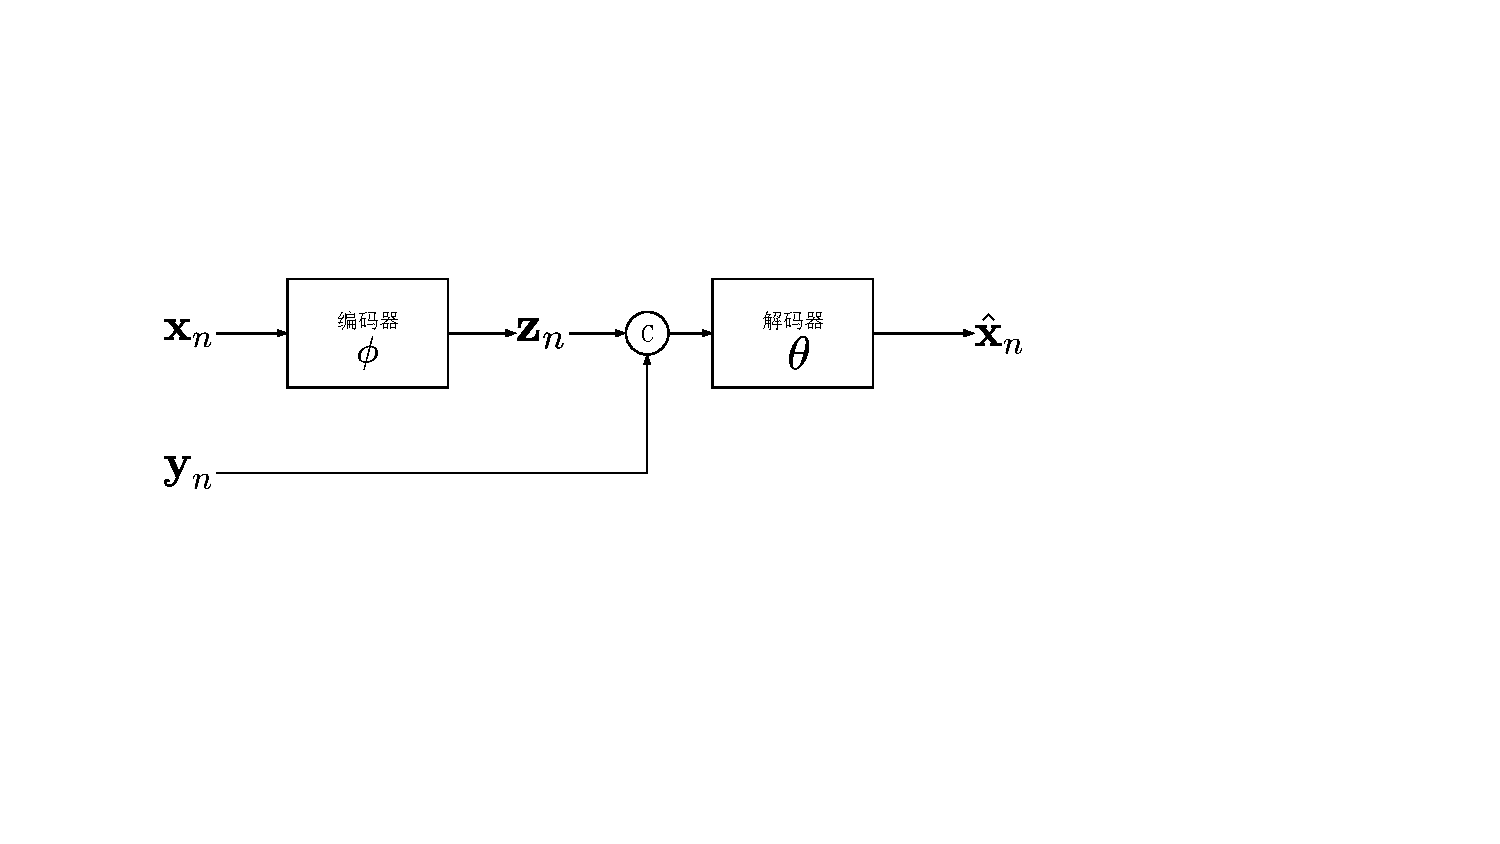
\includegraphics[width=13cm,trim=30 170 170 130,clip]{figure/3_vae.pdf}
    \bicaption[变分自编码器语音转换方法示意图]
    {变分自编码器语音转换方法示意图}
    {Schematic diagram of the VAE Voice Conversion method}
    \label{fig:vae}
\end{figure}

基于变分自编码器(Variational AutoEncoder, VAE)的语音转换方法于2016年被提出。VAE同生成对抗模型类似,也是生成模型的一种。
如图~\ref{fig:vae}所示,VAE可以分为编码器$\phi$和解码器$\theta$两个模型,其中编码器将输入的声学特征$\mathbf{x}_n$转换为说话人无关的隐变量$\mathbf{z}_n$:

\begin{equation}
    \mathbf{z}_n = f_{\phi}(\mathbf{x}_n)
\end{equation}

此时隐变量只包含说话人无关的信息,例如音素,韵律等。之后,用解码器将隐变量恢复为最初的输入$\mathbf{x}_n$,为此,需要额外添加说话人信息变量$\mathbf{y}_n$。
解码器以隐变量和说话人信息拼接之后的结果作为输入,即

\begin{equation}
    \hat{\mathbf{x}}_n = f_{\theta}(\mathbf{z}_n,\mathbf{y}_n)
\end{equation}

基于VAE的语音转换方法基于两个假设:一是说话人信息和说话人无关信息可以从一帧声学特征向量中解耦出来;二是解码器可以通过混合这两个信息来合成一个声学特征向量。
模型的最终目标函数可以表示为

\begin{equation}
    \hat{L}(\theta,\phi,x_n)=-D_{KL}(q_{\phi}(\hat{z}_n|x_n)||p(z_n))+logp_{\theta}(x_n|\hat{z}_n,y_n)
\end{equation}

在转换过程中,编码器首先将输入帧转变为隐向量,然后解码器输入隐向量和目标说话人向量来输出转换特征帧。


\section{基于CycleGAN的语音转换方法}
本文所做的语音转换工作主要基于CycleGAN的语音转换方法,本节将先简要介绍该方法涉及到的基本概念如对偶学习,生成对抗网络等,
之后对CycleGAN的原理及其在语音转换上的优化进行详细说明。

\begin{figure}[!htp]
    \centering
    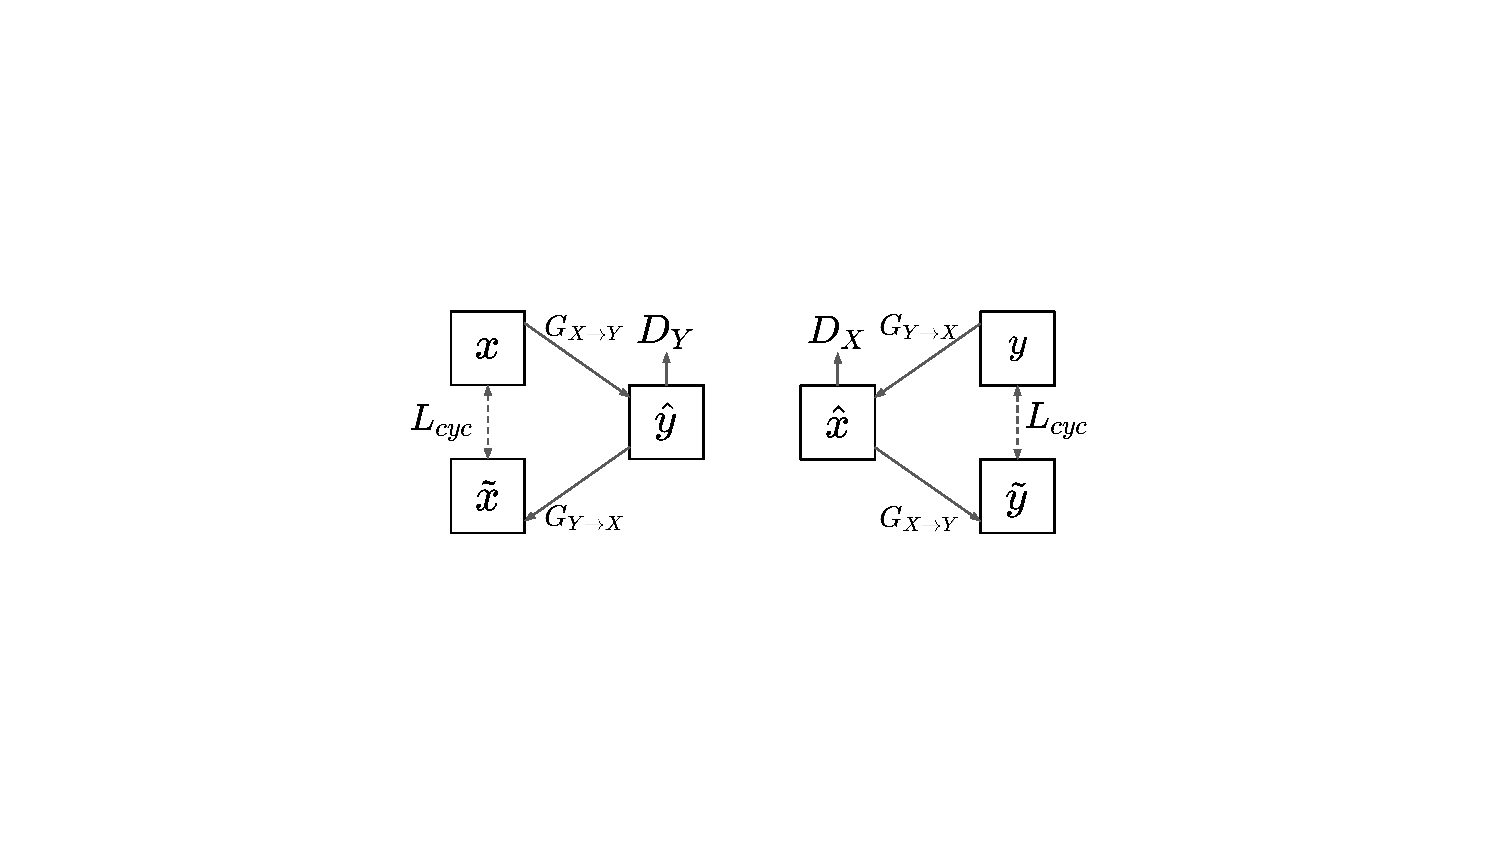
\includegraphics[width=13cm,trim=100 140 100 140,clip]{figure/3_cyclegan.pdf}
    \bicaption[标准CycleGAN示意图]
    {标准CycleGAN示意图}
    {Schematic diagram of the standard CycleGAN}
    \label{fig:cyclegan}
\end{figure}

\subsection{对偶学习概述}
对偶学习(Dual Learning)的概念最早于2016年提出\cite{he2016dual}。以神经网络为代表的深度学习技术
近两年在许多领域内都取得了巨大的成功,其中一个重要的因素就是大数据,尤其是大规模的经过标注的数据。例如
在语音合成中,神经网络通常需要上万句带有标注的音频样本来学习文本到声学特征之间的关系,这些数据需要
大量人工对其进行标注,校对等工作,极大增加了一个模型的构建成本。这个问题在机器翻译领域尤为突出,在机器
翻译中,会用到上千万的双语句对进行训练,这对数据的收集和标注都提出了很大的挑战。深度学习技术的广泛性
与其对大规模标注数据的依赖性有很大的关系。为了解决这个问题,研究人员提出了一种新的学习范式,即对偶学习。

可以发现,很多深度学习的任务都可以衍生出一个对偶任务,如机器翻译的中译英和英译中,语音转换的原始说话人转目标说话人和
目标说话人转原始说话人,甚至语音识别和语音合成。这些互为对偶的深度学习任务可以形成一个闭环,使从没有标注的数据中学习
模型成为可能。对偶学习最重要的一点是,对于一个主任务,其对偶任务可以给其反馈,反过来主任务也可以给对偶任务以反馈,从而
实现两个任务相互反馈,相互学习。

实际上对偶学习与强化学习的学习过程较为相似。在强化学习中,并没有标注样本来告诉模型在某个状态执行某个动作是正确的,模型
只有通过使用策略在某个状态下执行不同的动作,观测该动作带来的回报,从而改善策略。在对偶学习中,两个对偶任务就是策略,
模型输入就是状态,两次模型的输出就是动作,而重建误差就是动作带来的回报。

以中英机器翻译为例,已有预训练或未训练的英译中模型$f$和中译英模型$g$,给定一个英文句子$x$,首先用英译中模型$f$将该句翻译成中文$y^{'}$,
然后将该中文句子$y^{'}$发送给中译英模型$g$。中译英模型$g$并不知道正确的翻译是什么,但可以知道这个中文句子语法是否正确,
是否符合中文语言模型,这些信息都可以帮助中译英模型$g$判断英译中模型$f$是否做的好。然后中译英模型$g$翻译成英文句子$x^{'}$,
通过比较$x$和$x^{'}$是否相似,就可以判断两个模型$f$和$g$做的是不是足够好,尽管输入$x$是一个没有标注的句子。同理,也可以输入
中文句子,使其分别通过中译英模型$g$和英译中模型$f$,来实现重建。因此,通过
这样的一个对偶游戏的过程,就能够从没有标注的数据上获得反馈,从而提高模型性能。

对偶学习同样可以应用在语音转换中,对于语音转换而言,原始说话人和目标说话人可以互相调换,来得到对应的对偶任务。
为了训练从说话人$A$到说话人$B$的语音转换模型$G$,需要同时学习转换模型$G_{A\rightarrow B}$和$G_{B\rightarrow A}$。
分别输入两个说话人的原始特征,通过两个模型对原始特征进行重构,将重构误差作为回报帮助两个模型训练。但是仅有重构误差对于语音转换
的对偶学习来说还是不够的,因为两个模型很容易都训练成将输入原样输出来使重构误差最小,为了解决这个问题,需要在每次循环中对第一个模型
的输出加入约束,强制其输出符合目标说话人的特征分布。

\subsection{生成对抗网络简介}
生成对抗网络(Generative Adversarial Networks, GAN)由Ian Goodfellow等人于2014年提出\cite{goodfellow2014generative}。
迄今为止GAN已经在许多生成式任务中实现了非常好的效果,如图像生成,自然语言生成和音乐声称等。该模型从一个游戏理论中获得启发:两个模型,
一个生成器(Generator),一个判别器(Discriminator),在互相竞争的过程中彼此越来越强大。然而,GAN的训练是较为困难的,研究人员在训练过程中经常遇到不稳定和模型不收敛的问题。

GAN包含两个模型:判别器$D$对输入样本进行判断,并输出该样本属于真实数据集的概率,判别器像一个裁判,其优化目标是对真实
样本尽可能高的概率值,同时对合成样本较低的概率值。生成器$G$输入噪声变量$z$,输出合成样本,生成去的训练目标是尽可能生成接近
真实数据分布的合成样本,以至于可以欺骗判别器,使其给出较高的概率值。在训练过程中,两个模型在这个零和游戏中互相对抗,并不断提升彼此的能力。

一方面,判别器$D$确保在真实数据上足够准确,通过最大化$\mathbb{E}_{x\sim p_r(x)}\left[log D(x)\right]$,同时,输入一个假的样本
$G(z)$,$z\sim p_z(z)$,判别器期望输出其概率$D(G(z))$尽可能接近$0$通过最大化$\mathbb{E}_{z\sim p_z(z)}\left[log(1-D(G(z)))\right]$。
在另一方面,生成器希望提升判别器对其生成的样本的概率值通过最小化$\mathbb{E}_{z\sim p_z(z)}\left[log(1-D(G(z)))\right]$。将两个目标函数
合并,可以得到需要优化的损失函数

\begin{equation}
    \min_G \max_D L(D,G)=\mathbb{E}_{x\sim p_r(x)}\left[log D(x)\right] + \mathbb{E}_{z\sim p_z(z)}\left[log(1-D(G(z)))\right]
\end{equation}

其中等号右边的第一项对生成器$G$训练时没有影响。通过对损失函数在所有x上求导,可以得到对于判别器而言,其使损失函数最低的最优概率值为0.5,整个
损失函数的全局最优值为$-2log2$。GAN的发展至今已经演变出很多种类,包括加入条件的条件GAN,使用最小二乘法的LSGAN,以及引入对偶学习的CycleGAN,StarGAN等。

\subsection{CycleGAN网络的训练}
CycleGAN网络包含四个模型,两个生成器($G_{X\rightarrow Y}$,$G_{Y\rightarrow X}$)和两个判别器($D_X$,$D_Y$),$X$和$Y$分别代表原始域和目标域。
四个模型通过两个个损失函数来实现无监督的训练:对抗损失(Adversarial Loss)和重构损失(Reconstruct Loss)。
其中对抗损失用来衡量转换的目标特征和真实的目标特征之间的区分程度。判别器通过最大化对抗损失来尽可能区分转换特征和真实特征,
同时生成器通过最小化对抗损失来尽可能生成接近真实的转换特征,从而欺骗判别器。其训练方式与生成对抗网络类似,
生成器和判别器交替训练更新,训练生成器时判别器只回传梯度,不更新梯度。对抗损失表示如下

\begin{align}
    L_{adv}(G_{X\rightarrow Y},D_Y) & =\mathbb{E}_{y\sim P_{Data}(y)}\left[log D_Y(y)\right] \\
    & + \mathbb{E}_{x\sim P_{Data}(x)}\left[log(1-D_Y(G_{X\rightarrow Y}(x)))\right] \\
    L_{adv}(G_{Y\rightarrow X},D_X) & =\mathbb{E}_{x\sim P_{Data}(x)}\left[log D_X(x)\right] \\
    & + \mathbb{E}_{y\sim P_{Data}(y)}\left[log(1-D_X(G_{Y\rightarrow X}(y)))\right] 
\end{align}


对于重构损失,域$X$中的每一个样本$x$都可以通过主任务和对偶任务(或交换)的级联重新恢复为$x$,因此重构损失可以表示为

\begin{align}
    L_{cyc}(G_{X\rightarrow Y},G_{Y\rightarrow X}) & = \mathbb{E}_{x\sim P_{Data}(x)}\left[\left| \left| G_{Y\rightarrow X}(G_{X\rightarrow Y}(x))\right| \right|_1 \right] \\
    & + \mathbb{E}_{y\sim P_{Data}(y)}\left[\left| \left| G_{X\rightarrow Y}(G_{Y\rightarrow X}(y))\right| \right|_1 \right]
\end{align}

如图~\ref{fig:cyclegan}所示,输入依次经过两个级联的生成器后,得到的输出和输入计算重构损失,之后梯度沿着两个生成器反向传播,
并对两个生成器同时更新参数。对两个损失函数加入权重后,最终的损失函数为

\begin{align}
    L_{full}& =L_{adv}(G_{X\rightarrow Y},D_Y)+L_{adv}(G_{Y\rightarrow X},D_X)\\
    & +\lambda_{cyc}L_{cyc}(G_{X\rightarrow Y},G_{Y\rightarrow X})
\end{align}

\subsection{门控卷积网络和身份损失}
为了将CycleGAN应用到语音转换中,作者提出了在网络中使用门控卷积网络(Gated CNN)以及一个额外的身份损失函数(Identity Loss)。
语音中的一个主要特性就是语音中含有序列和层级的结构关系,例如发声和不发声(voiced/unvoiced),音素和词素(phonemes/morphemes)。
一个对该特性建模的有效方法是使用RNN,但是RNN在训练和计算速度上都不如CNN。因此作者提出在CycleGAN中使用门控卷积网络。门控卷积网络
既可以在序列数据上并行计算,同时也在语言和语音建模上较为成功。在门控卷积网络中,选用门控线性单元(Gated Linear Unit, GLU)作为激励函数。
GLU计算过程公式表示为

\begin{equation}
    \mathbf{H}_{l+1}=(\mathbf{H}_l \ast \mathbf{W}_l + b_l)\otimes \sigma (\mathbf{H}_l \ast \mathbf{V}_l + c_l)
\end{equation}

其中$\mathbf{W}$,$\mathbf{V}$,$b$和$c$是模型参数,$\mathbf{H}_l$是$l$层的输出,$\otimes$是逐元素乘法。门控机制可以允许信息被
选择性地传播到下一层。

身份损失通常只用来在训练的开始阶段使用,其作用为在训练开始时尽可能缩小生成器的参数空间。
该损失函数的提出考虑到对于语音转换任务而言,只需考虑转换说话人信息,而语音中的主要信息(如文本)是不改变的。
因此在训练开始时首先尽可能保证生成器保留语音中的所有信息,之后再对其中的说话人信息进行着重调整,
身份损失能够有效加速模型收敛和保留语义。为了保证生成器的输出始终在目标说话人的特征分布内,
身份损失选择输入目标特征而非原始特征。公式如下

\begin{align}
    L_{id}(G_{X\rightarrow Y},G_{Y\rightarrow X}) & = \mathbb{E}_{y\sim P_{Data}(y)}\left[\left| \left| G_{X\rightarrow Y}(y)-y\right| \right|_1 \right] \\
    & + \mathbb{E}_{x\sim P_{Data}(x)}\left[\left| \left| G_{Y\rightarrow X}(x)-x\right| \right|_1 \right]
\end{align}

\section{本章小结}
本章首先介绍了非平行语音转换及其常见方法,包括音素后验概率图法,对抗训练法和变分自编码器法,并对本文中用到的基于CycleGAN的语音转换方法
进行了详细的介绍。标准的CycleGAN中计算重构损失时,级联的两个生成器同时进行前向和后向传播。
在该设置下,转换音频通常包含有较多噪音,从而会导致较低的语音自然度和说话人相似度。
下一章将会从更新过程的角度进一步分析标准CycleGAN的训练过程,并介绍所提出的半优化CycleGAN和基频辅助特征来提升模型性能。

\chapter{基于半优化CycleGAN的非平行语料语音转换}

\section{引言}
上文介绍了非平行语料语音转换的基本概念及其常见方法,并详细介绍了基于CycleGAN的语音转换方法。
尽管这些方法极大地推动了非平行语料语音转换的技术发展,但是在目前的相关技术里转换语音的音质依旧存在较大的提升空间。

本章基于CycleGAN提出了一种改进的语音转换框架,该框架主要包含两个改进:半优化的CycleGAN模型 (Semi-optimized CycleGAN) 
和基频辅助特征;同时为了提升音质,该框架使用WaveNet声码器替代传统声码器,使用梅尔频谱特征代替传统的梅尔倒谱特征。
半优化CycleGAN主要特性为两个非一致更新的生成器,即在训练过程中,每个循环只有一个生成器被更新,另一个生成器只被用来生成中间特征。
经过对每个生成器的更新过程进行分析,在标准CycleGAN中,部分更新过程会导致生成器在计算损失时受到带有噪声标签的影响,
并且不同的更新过程之间存在互斥现象,从而导致转换模型性能的下降。半优化CycleGAN即通过去除该部分更新过程来提升模型性能。
参考近年语音合成和语音转换在声码器方面的研究,我们使用梅尔频谱作为声学特征,
来替代传统的梅尔倒谱系数、非周期信息和基频这三个特征,并使用基于梅尔频谱的WaveNet模型作为声码器。
为了克服CycleGAN模型对梅尔频谱中音调信息的学习能力不足的问题,提出在训练过程中使用基频特征作为梅尔频谱特征的辅助特征来共同训练,
该改进在保持使用梅尔频谱作为WaveNet的特征下,有效解决了转换音频中音调错误的问题。
本章将首先详细介绍基于梅尔频谱的WaveNet声码器在语音转换中的应用,然后阐述所提出的包含半优化CycleGAN和基频辅助特征的非平行语料语音转换系统,
最后对实验配置和实验结果进行说明和分析。

\section{基于梅尔频谱WaveNet的平行语料语音转换}
\subsection{WaveNet声码器}
如上文所述,WaveNet是一种自回归的概率生成模型,该模型可以通过历史音频样本点,直接预测当前样本点的分布,其模型结构如图~\ref{fig:wavenetarch}所示

\begin{figure}[!htp]
    \centering
    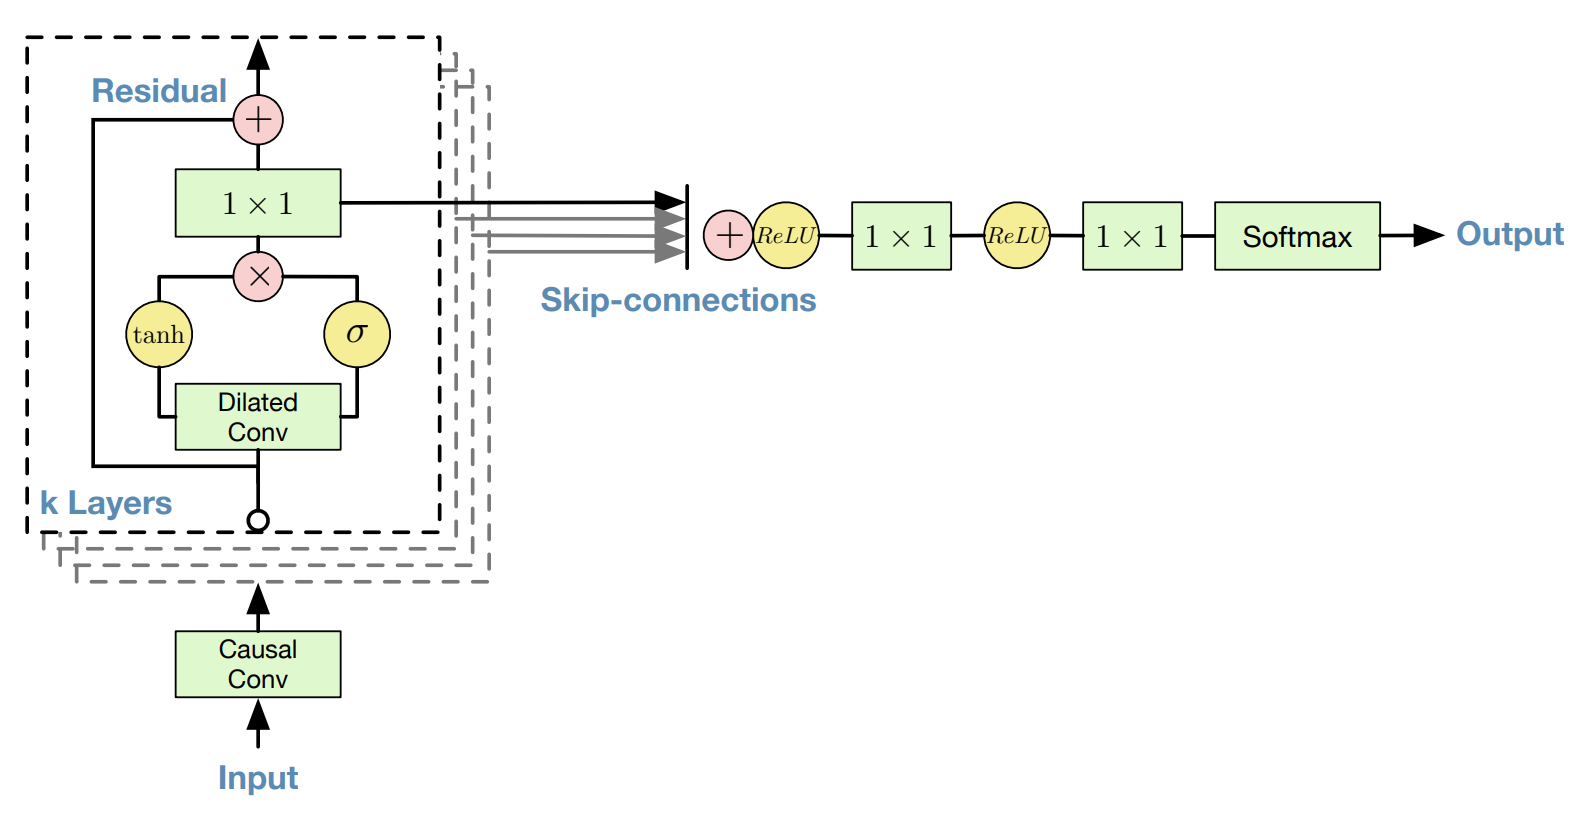
\includegraphics[width=12cm,trim=0 10 0 0,clip]{figure/4_wavenet.png}
    \bicaption[WaveNet模型结构图\cite{oord2016wavenet}]
    {WaveNet模型结构图}
    {Architecture of the WaveNet}
    \label{fig:wavenetarch}
\end{figure}

其中因果卷积 (Causal Conv) 和扩张卷积 (Dilated Conv) 可以有效增加模型的输入感受域。模型由多个跳跃连接模块构成,每个模块
包含一个扩张卷积和门控激励函数,其中的$1*1$代表卷积核大小为1x1的卷积网络。每个模块的输出可以表示为

\begin{equation}
    \mathbf{z} = tanh(W_{f,k} * \mathbf{x} + V^{T}_{f,k}\mathbf{h})\odot \sigma(W_{g,k} * \mathbf{x} + V^{T}_{g,k}\mathbf{h})
\end{equation}

其中$\mathbf{x}$和$\mathbf{z}$分别为输入和输出向量,$k$代表层编号,$f$和$g$分别代表门控激励函数中的滤波器和门,$W_{f,k}$,$W_{g,k}$,$V^T_{f,k}$,$V^T_{g,k}$
是可学习的权重矩阵,$*$是卷积操作,$\odot$是逐元素的乘法操作,$\sigma$是$sigmoid$函数,$h$表示全局条件向量。全局条件向量在WaveNet生成过程保持不变,常用于多说话人模型
中的说话人条件。对于局部特征来说,条件特征从单个向量变为了第二个特征序列$h_t$,该序列通常以帧为单位,因此采样率会低于音频信号,例如语音合成系统中的语义特征或者声码器中的声学特征。
通常会先将局部条件特征序列通过转置卷积或重复操作来将条件特征的采样率调整至与音频信号相同$\mathbf{y} = f(\mathbf{h})$,然后每一个模块的输出可变为

\begin{equation}
    \mathbf{z} = tanh(W_{f,k} * \mathbf{x} + V_{f,k} * \mathbf{y}) \odot \sigma (W_{g,k} * \mathbf{x} + V_{g,k} * \mathbf{y})
\end{equation}

此时$V_{f,k} * \mathbf{y}$和$V_{g,k} * \mathbf{y}$是一个1x1卷积层。整个网络的最终输出是一个$softmax$层,输出一个
256维度的概率向量。因为音频的采样点通常是浮点数,为了能够降低建模复杂度,需要首先用mu-law算法将浮点采样点分为256类,
将音频转换为一个256维的特征向量序列,具体公式如下

\begin{equation}
    f(x_t) = sign(x_t)\frac{ln(1+\mu \left| x_t\right|)}{ln(1+\mu)}
\end{equation}

其中$x_t$为t时刻的采样点,值域为$\left[-1,1\right]$ $sign$函数返回$x_t$的正负符号,$\mu$代表压缩的类别数,这里$\mu$取256。


\subsection{梅尔频谱特征转换}

\begin{figure}[!hbtp]
    \centering
    \bisubcaptionbox{传统语音转换}%
                    {Conventional Voice Conversion}%
                    [14cm]{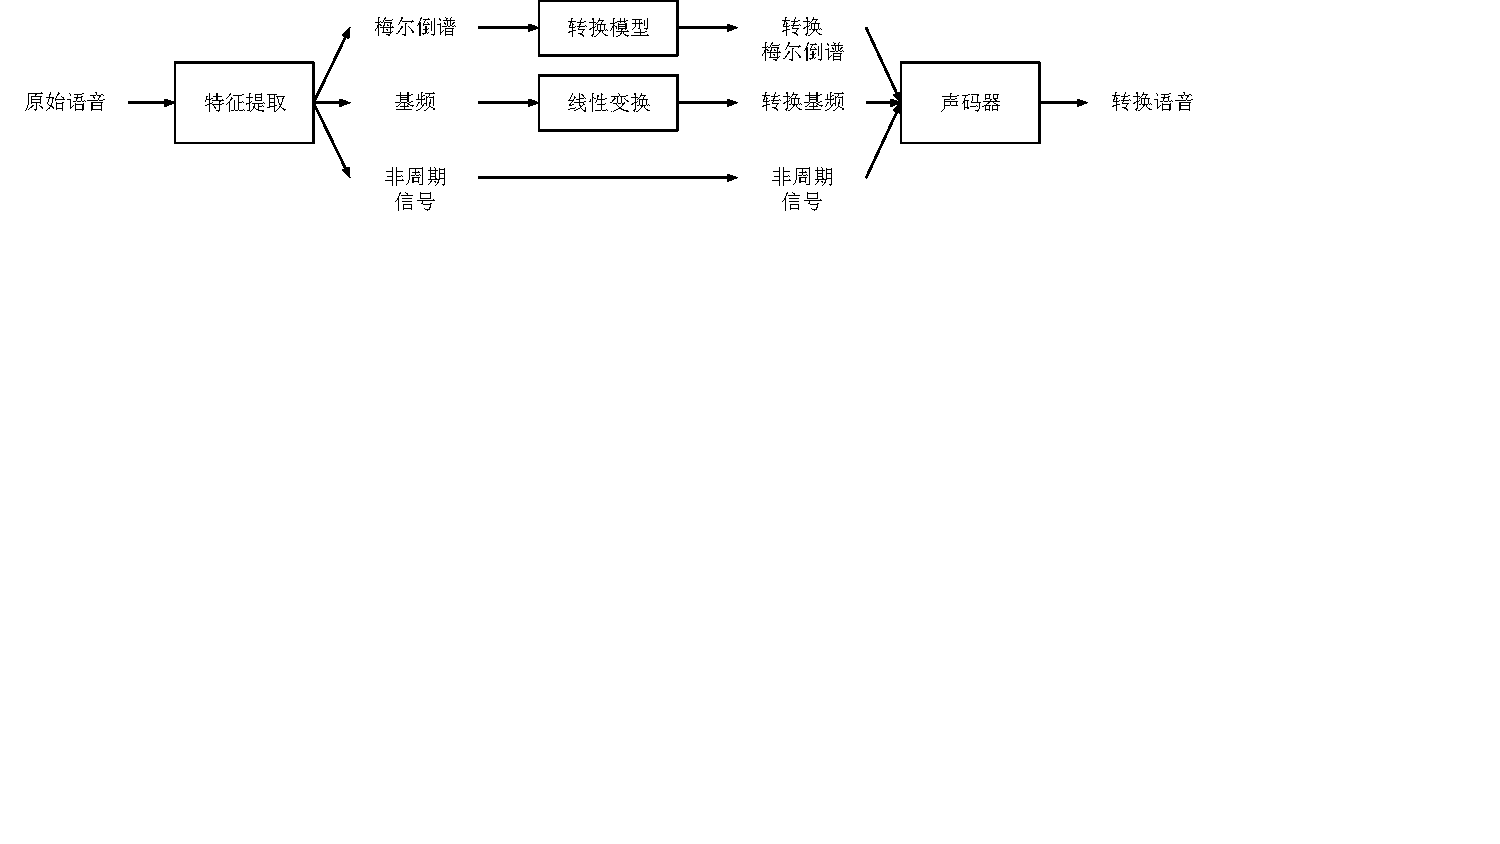
\includegraphics[width=14cm,trim=0 300 140 0,clip]{figure/4_vcmcep.pdf}} \\
    \vspace{0.5cm}
    \bisubcaptionbox{基于梅尔频谱的语音转换}%
                    {Mel-spectraogram based Voice Conversion}%bisubcaptionbox
                    [14cm]{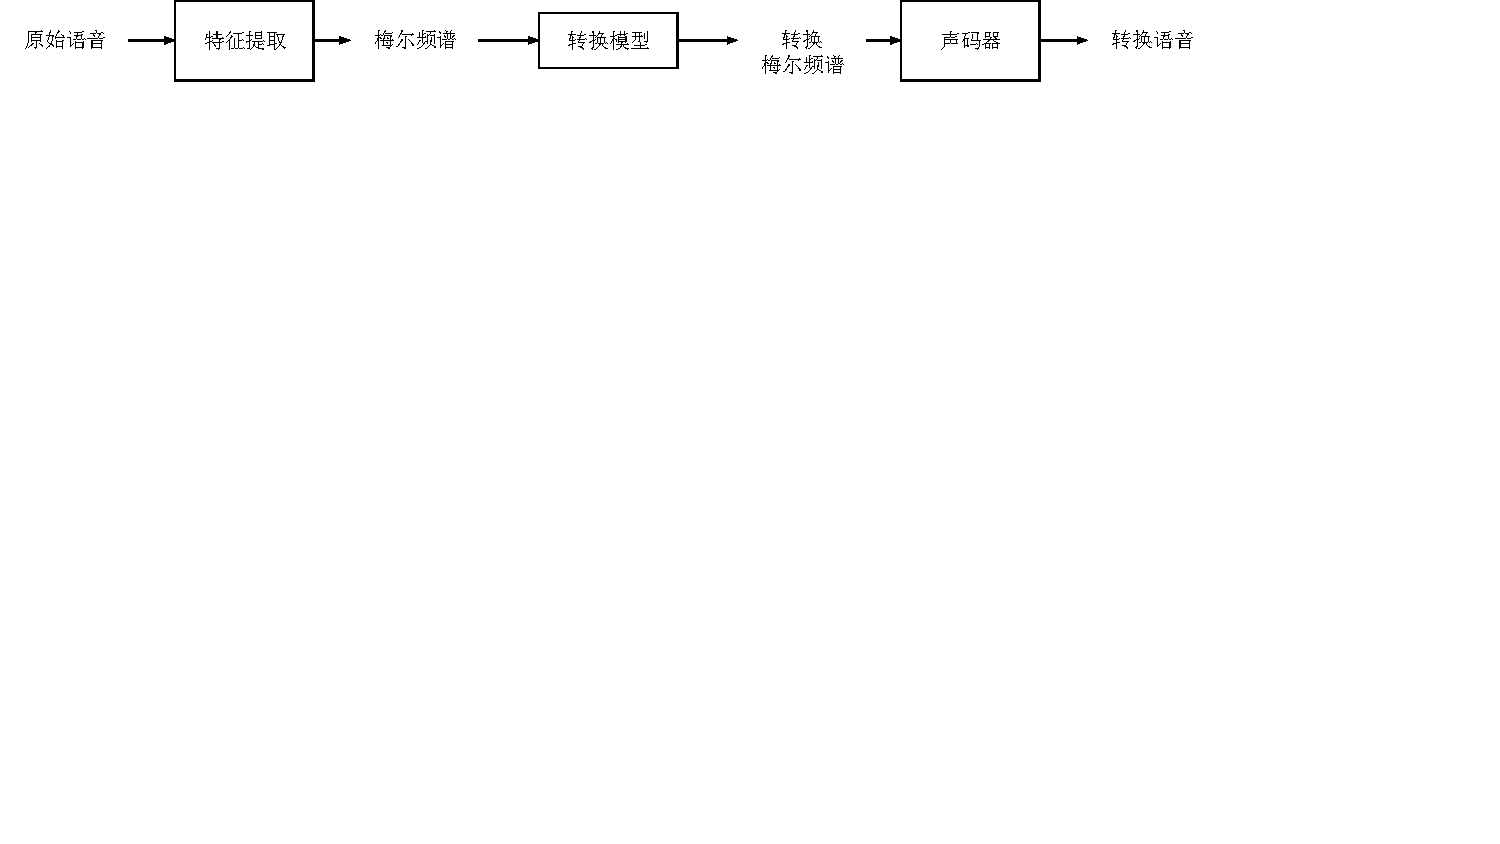
\includegraphics[width=14cm,trim=0 350 140 0,clip]{figure/4_vcmsp.pdf}}
    \bicaption{梅尔频谱语音转换和传统语音转换对比图}
              {Comparison of the Mel-spectrogram based Voice Conversion and the conventional Voice Conversion}
    \label{fig:vcdiff}
  \end{figure}

对于基于梅尔频谱的语音转换,可以使用任何转换模型将原始说话人的梅尔频谱特征转换为目标说话人,再通过WaveNet生成波形。
该方法与传统语音转换方法的区别如图~\ref{fig:vcdiff}所示,在传统的语音转换中,通过传统声码器会从语音中提取三个特征:梅尔倒谱系数 (Mgc) ,非周期信号 (bap) 和基频 (F0) 。
其中Mgc使用转换模型进行转换,bap保持不变,F0使用线性变换。
处理后的三个特征再通过数字信号声码器或神经网络声码器进行波形生成。
当使用梅尔频谱作为特征时,则直接从音频中提取梅尔频谱,然后将其作为转换特征进行训练和转换,声码器也直接从梅尔频谱中恢复波形。
梅尔频谱是将频谱映射到梅尔刻度 (Mel scale) 后取前$k$维得到的特征,梅尔刻度是基于彼此等距的听众对音高 (pitch) 的感性判断的刻度。

在\cite{chen2018high}中,作者在平行语料的语音转换任务中对比了
不同声学特征和声码器配置下转换语音的性能。
图~\ref{fig:wavenetworld4}为自然度主观意见分实验,其中bdl-slt和clb-slt分别为跨性别说话人组和同性别说话人组。在所示的
各组对照组中,N为自然音频,WNS为真实梅尔频谱特征的WaveNet合成音,WNC为真实梅尔倒谱特征的WaveNet合成音,WCS为转换
梅尔频谱的WaveNet合成音,WCC为转换梅尔倒谱特征的WaveNet合成音,MCC为转换梅尔倒谱特征的STRAIGHT合成音。可以看出
在梅尔倒谱特征中,STRAIGHT表现要优于WaveNet,但基于梅尔频谱的WaveNet不论在反合成还是在转换特征上合成,自然度都要好于
数字信号声码器。图~\ref{fig:wavenetworld1}和图~\ref{fig:wavenetworld2}展示了对转换语音相似度的偏好测试结果,可以看出不论是同性别还是跨性别上,
基于梅尔频谱的WaveNet (Msp WaveNet) 都要明显好于基于梅尔倒谱的WaveNet (Mcep WaveNet) 和STRAIGHT (Mcep STRAIGHT) 。


% \begin{figure}[!htp]
%     \centering
%     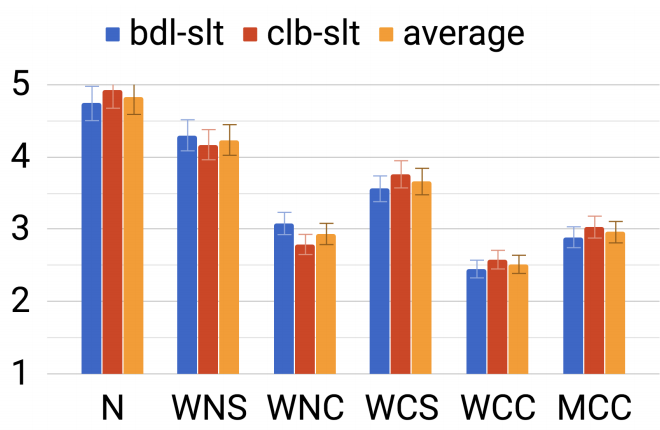
\includegraphics[width=10cm,trim=0 0 0 0,clip]{figure/4_wavenetworld4.png}
%     \bicaption[不同特征和声码器下转换语音的自然度对比\cite{chen2018high}]
%     {不同特征和声码器下转换语音的自然度对比}
%     {Comparison of converted speech naturalness on different features and vocoders}
%     \label{fig:wavenetworld4}
% \end{figure}

% \begin{figure}[!hbtp]
%     \centering

%     \bisubcaptionbox{相似度同性别}%
%                     {Intra-gender}%
%                     [10cm]{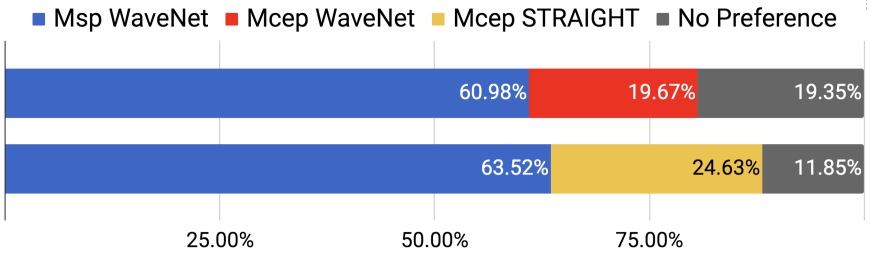
\includegraphics[width=10cm,trim=0 0 0 0,clip]{figure/4_wavenetworld1.png}} \\
%     \vspace{0.5cm}
%     \bisubcaptionbox{相似度跨性别}%
%                     {Inter-gender}%bisubcaptionbox
%                     [10cm]{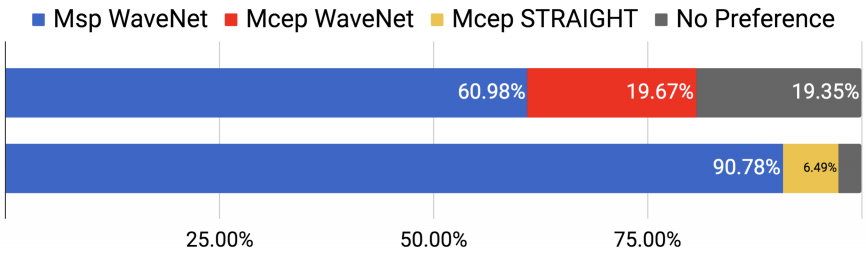
\includegraphics[width=10cm,trim=0 0 0 0,clip]{figure/4_wavenetworld2.png}}
%     \bicaption{不同特征和声码器下语音转换偏好测试对比图\cite{chen2018high}}
%               {Preference test on Voice Conversion of different features and vocoders}
%     \label{fig:wavenetworld1}
%   \end{figure}

\begin{figure}[!ht]
    \begin{subfigure}[b]{0.48\linewidth}
        %\rule{\linewidth}{1\linewidth}
        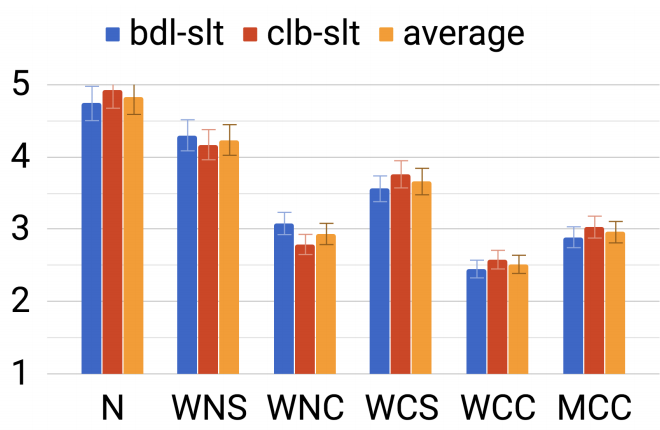
\includegraphics[width=\linewidth,trim=0 0 0 0,clip]{figure/4_wavenetworld4.png}

        \bicaption[MOS自然度]
        {MOS自然度}
        {Comparison of speech naturalness}
        \label{fig:wavenetworld4}
    \end{subfigure}
    \hfill
    \begin{minipage}[b]{0.5\linewidth}
        \begin{subfigure}[b]{\linewidth}
            %\rule{\linewidth}{0.5\linewidth}
            \centering
            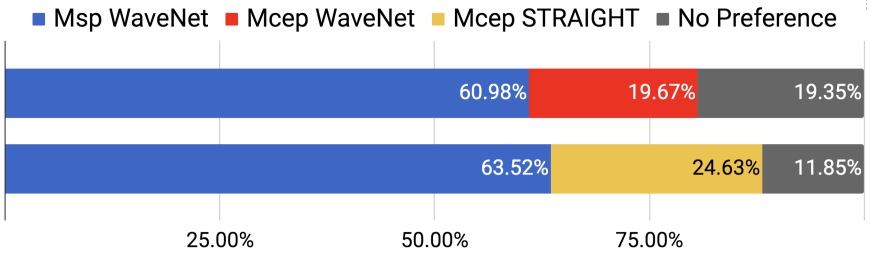
\includegraphics[width=0.8\linewidth,trim=0 0 0 0,clip]{figure/4_wavenetworld1.png}
            \bicaption[相似度同性别]{相似度同性别}{Intra-gender Similarity}
            \label{fig:wavenetworld1}
        \end{subfigure}\\
        \begin{subfigure}[b]{\linewidth}
            \centering
            %\rule{\linewidth}{0.5\linewidth}
            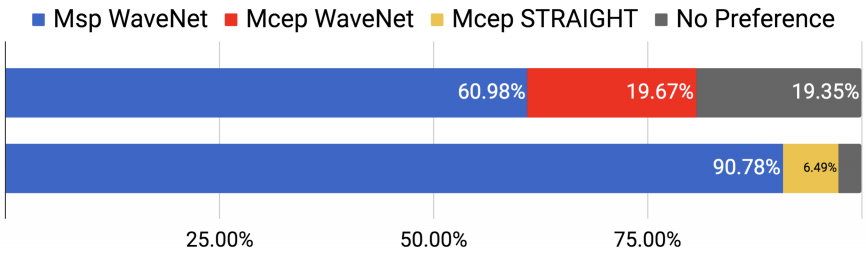
\includegraphics[width=0.8\linewidth,trim=0 0 0 0,clip]{figure/4_wavenetworld2.png}
            \bicaption[相似度跨性别]{相似度跨性别}{Inter-gender Similarity}
            \label{fig:wavenetworld2}
        \end{subfigure}
    \end{minipage}
    \bicaption{不同特征和声码器下语音转换对比图\cite{chen2018high}}
    {Comparison on Voice Conversion of different features and vocoders}
    \label{fig:wavenetworld}
\end{figure}

不同于梅尔倒谱,梅尔频谱不光包含了内容信息,还包含了音调信息,
相当于将传统的三个特征整合到了一起。因此,当使用梅尔频谱作为声学特征时,基频信息被隐性转换,
因此该转换会比线性转换拥有更复杂的音调转换能力,如前文所述,在平行语音转换中,先前的工作已经证明了在有监督的条件下,
梅尔频谱的音调转换能力要优于线性变换。但在无监督的条件下,由于没有真实标签,
同时CycleGAN的训练方式限制了生成器对局部信息的转换,导致模型较难从梅尔频谱中学习到基频表示。
因此基频的隐形转换拥有较大的难度。在我们的中文语音转换实验中,转换音频通常存在音调错误的问题,
尤其在男性转男性的实验中。我们提出使用基频辅助特征来提升模型的音调表示和转换能力,进而解决音调错误的问题。

\section{基于半优化CycleGAN的非平行语料语音转换系统}

\begin{figure}[!htp]
    \centering
    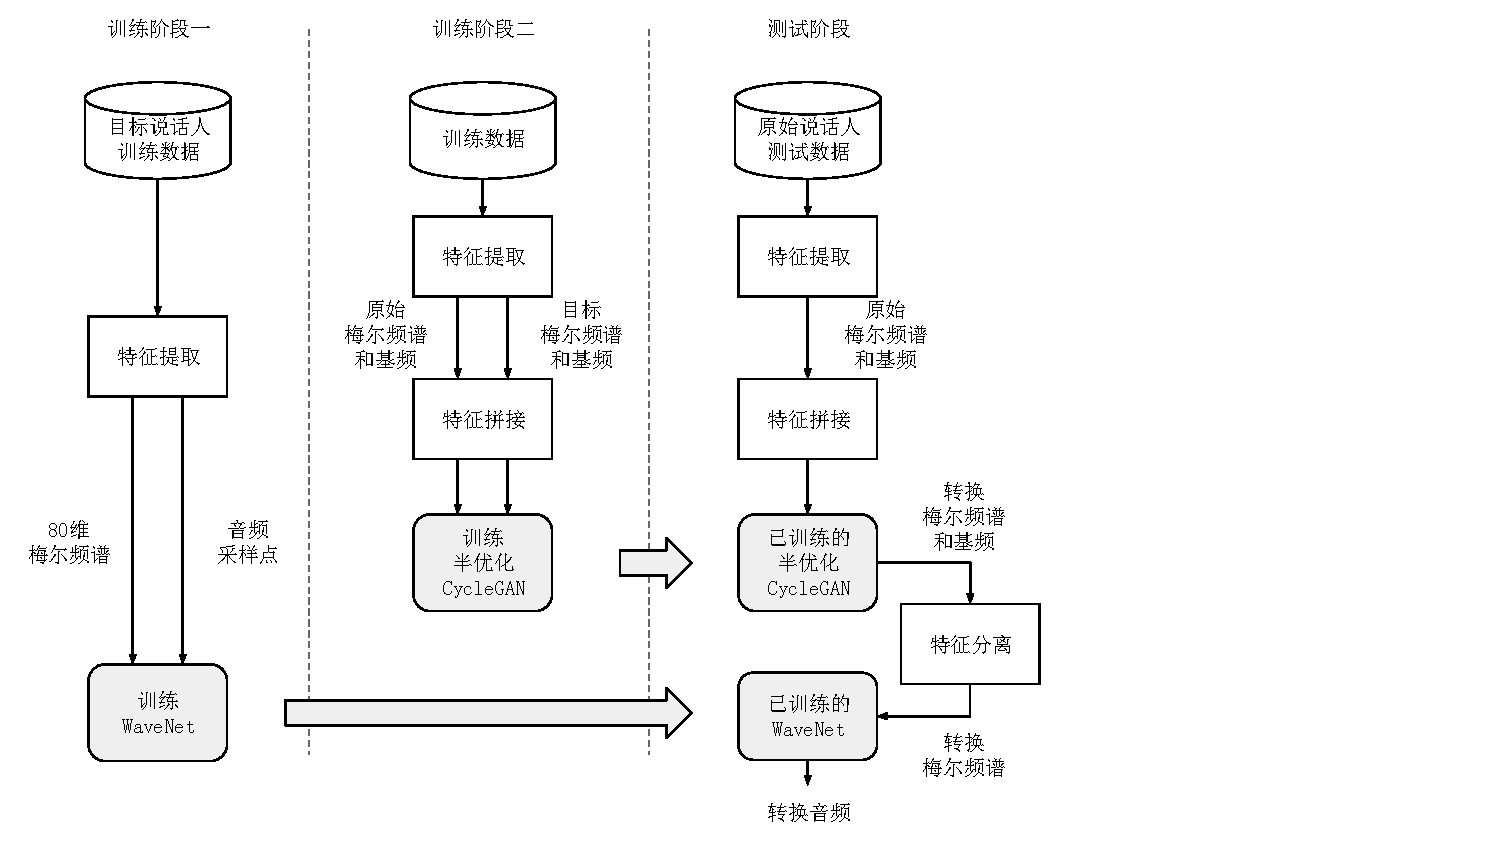
\includegraphics[width=12cm,trim=0 10 200 0,clip]{figure/4_proposedarch.pdf}
    \bicaption[基于半优化CycleGAN的语音转换系统结构图]
    {基于半优化CycleGAN的语音转换系统结构图}
    {Architecture of the semi-optimized CycleGAN based Voice Conversion}
    \label{fig:proposedarch}
\end{figure}

本文提出的改进框架,主要基于CycleGAN模型和基于梅尔频谱的语音转换,即:使用梅尔频谱作为声学特征,
CycleGAN作为语音转换模型,WaveNet作为神经网络声码器,以实现高音质的非平行语音转换。
结合上一节提出的现有框架的缺陷和不足,可以得出改进框架主要存在的两个挑战:
低音质的转换语音和非平行梅尔频谱转换中的发音错误问题。针对两个挑战,
本文分别提出半优化CycleGAN和基频辅助特征。在本节中,我们首先从最小更新过程的角度分析标准CycleGAN,
再介绍半优化CycleGAN。之后,再介绍使用基频辅助特征来解决音调转换错误的问题。

\subsection{半优化周期一致性生成对抗网络}

\begin{figure}[!htp]
    \centering
    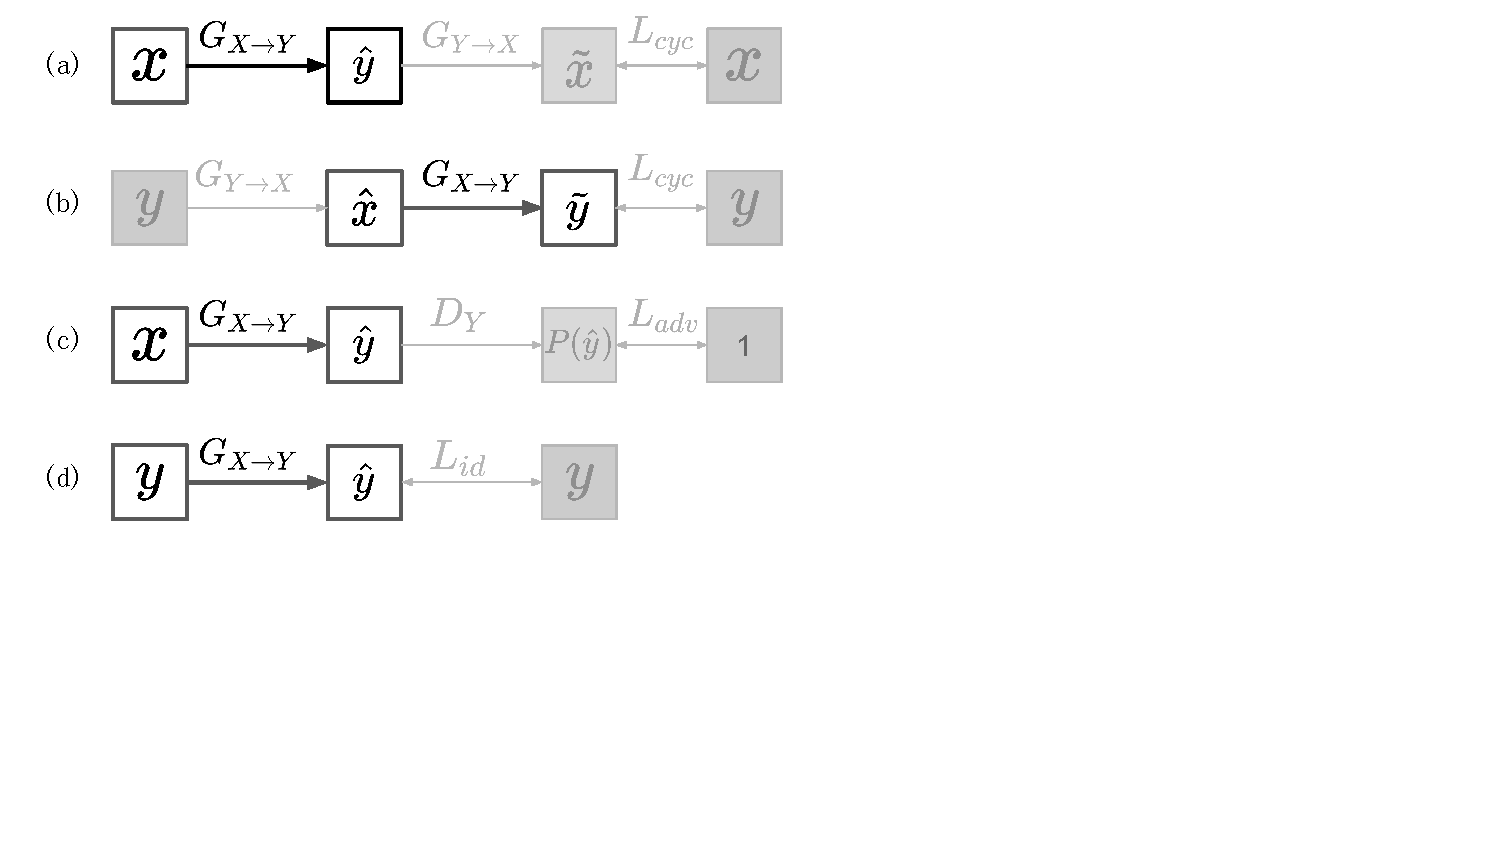
\includegraphics[width=8cm,trim=0 150 300 0,clip]{figure/4_dataflow.pdf}
    \bicaption[标准CycleGAN中最小更新过程示意图]
    {标准CycleGAN中最小更新过程示意图}
    {Schematic diagram of minimum update processes in conventional CycleGAN}
    \label{fig:dataflow}
\end{figure}

我们定义模型在训练过程中可以拆分的最小前向计算和反向梯度回传的过程作为一个最小更新过程。
从图~\ref{fig:dataflow}可以看出,对于每个生成器而言,一共有四个不同的最小更新过程来帮助模型训练,
其中(a)和(b)都来自于重构损失,(c)和(d)分别来自于对抗损失和身份损失。
这里我们只考虑单个生成器(以$G_{X\rightarrow Y}$为例)。
对每个最小更新过程进行分析,可以注意到对于(b)和(d),生成器的输出都有一个真实标签来计算损失。
然而对于(a)和(c),生成器是不存在一个真实的标签的,
并且其损失是由相连的下一个模型的梯度反传间接得到的。在(c)中,生成器和判别器对抗训练,
即当判别器尽可能去区分预测特征和真实特征时,生成器生成样本尽可能去欺骗判别器。
由于判别器本身在训练时存在样本和真实标签对,即真实特征和标签$1$。
因此通过对判别器输入预测特征,则可以得到预测特征和真实特征之间分布的误差。
该误差通过梯度反传至生成器的输出,则可以近似预测特征的损失,
使生成器的输出的数据分布更接近真实特征。然而,不同于(c),
(a)的下一个模型(即对偶的生成器$G_{Y\rightarrow X}$)并没有样本和真实标签对的训练数据,
因此经下一个模型反向传递的梯度无法保证能够很好地近似预测特征的损失;另一方面,
对偶的生成器在其身份损失的训练过程中(即更新过程(d)),
会输入和输出其目标特征,其反传的梯度会更接近于对偶生成器的目标特征分布,从而使得接近于,
这会影响当前模型训练,考虑到其可能带来的优点,更新过程(a)会对模型带来更多的负面影响。

\begin{figure}[!htp]
    \centering
    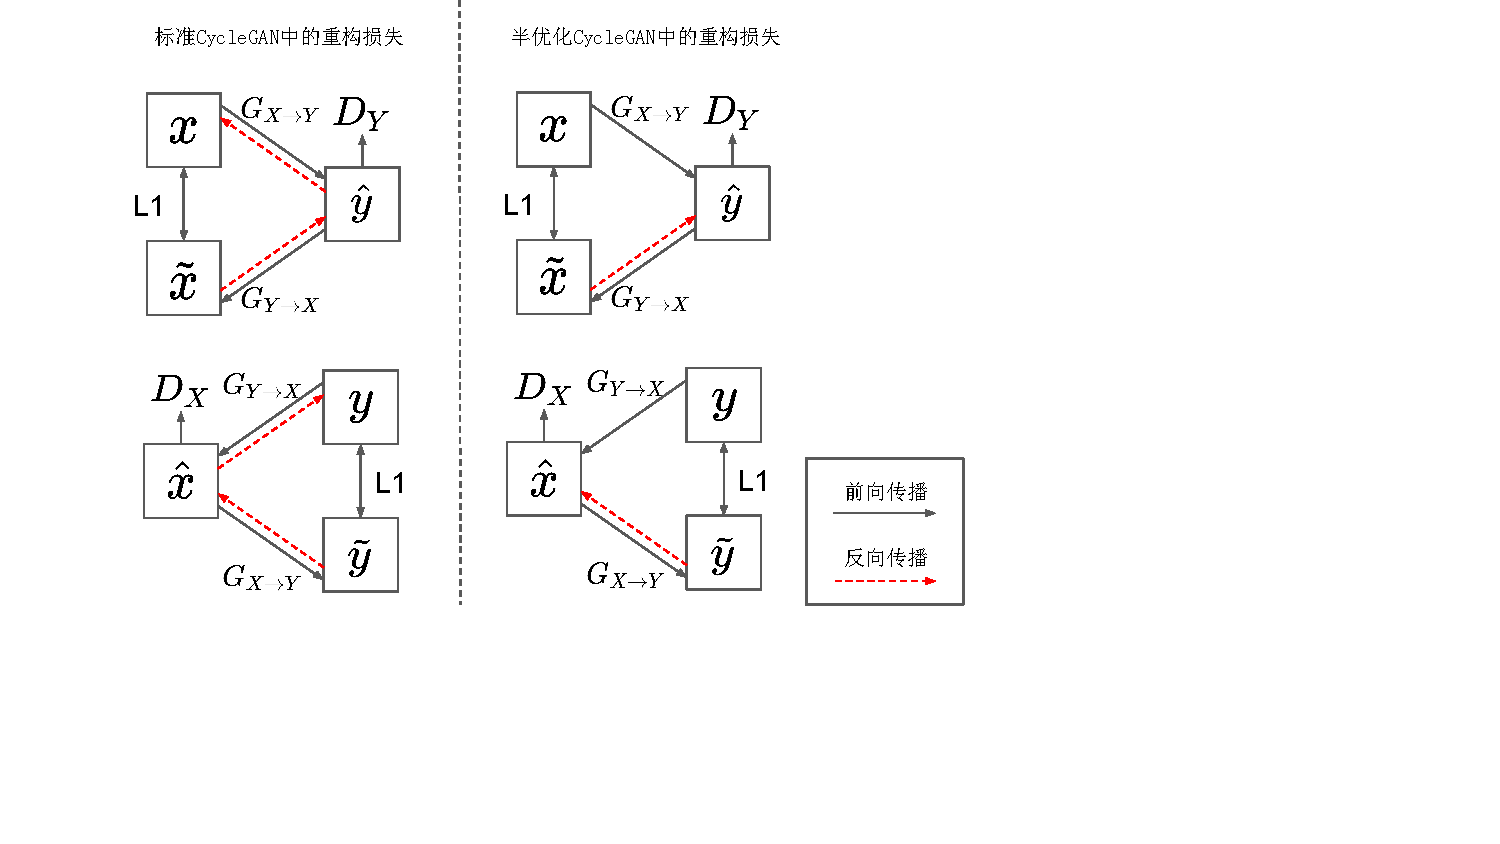
\includegraphics[width=10cm,trim=0 110 250 0,clip]{figure/4_semi.pdf}
    \bicaption[标准CycleGAN和半优化CycleGAN重构损失函数的对比图]
    {标准CycleGAN和半优化CycleGAN重构损失函数的对比图}
    {Comparison of Cycle-consistency loss between conventional CycleGAN and Semi-optimized CycleGAN}
    \label{fig:semi}
\end{figure}

因此我们对重构损失的训练策略进行了调整。如图~\ref{fig:semi}所示,我们去除了每个生成器的更新过程(a)。
因此对于每个循环,两个级联的生成器都会进行前向传播,但是只有第二个生成器会反向传播并更新,
此时第一个生成器只为第二个生成器生成带噪声的预测输入特征。我们称之为’半优化’。
重构损失公式变为

\begin{equation}
    L_{cyc}(G_{X\rightarrow Y},G_{Y\rightarrow X}) = L_{semicyc}(G_{X\rightarrow Y}) + L_{semicyc}(G_{Y\rightarrow X})
\end{equation}

其中

\begin{align}
    L_{semicyc}(G_{X\rightarrow Y}) & = \mathbb{E}_{y\sim P_{Data}(y)}\left[ \left| \left| G_{X\rightarrow Y}(G_{Y\rightarrow X}(y)) \right| \right|_1 \right] \\
    L_{semicyc}(G_{Y\rightarrow X}) & = \mathbb{E}_{x\sim P_{Data}(x)}\left[ \left| \left| G_{Y\rightarrow X}(G_{X\rightarrow Y}(x)) \right| \right|_1 \right]
\end{align}

在两次不同的循环中,分别只有一个生成器作为优化对象。
在实验中,我们发现半优化机制可以显著地减低噪声并提升转换语音自然度和说话人相似度。

\subsection{基频辅助特征}

我们使用梅尔频谱作为声学特征出于两个原因,一是其作为条件特征可以在WaveNet上生成相比梅尔倒谱和数字信号声码器更高音质的音频,
二是其本身包含了基频信息,因此可以使用神经网络进行更为复杂的基频隐性转换。然而如前文所述,
梅尔频谱直接作为CycleGAN的声学特征时存在发音错误的问题。主要原因分析如下。

如前文所述,
CycleGAN模型对说话人迁移的实现主要来自于对抗损失,其中判别器通过输入声学特征片段,
输出0到1之间的概率值来判断是否接近真实特征的分布。在经过大量的数据训练后,判别器能够对声学特征中的全局信息
(如说话人信息)有较强的判别能力,而随时间维度变化的局部信息(如语义,音调)在大量数据下很容易会被模型平均掉,
使模型对梅尔频谱中基频信息的表达学习较弱,从而导致转换特征存在发音错误的问题。理论上,如果加强判别器对序列建模的能力,如引入RNN,
可以使得模型对音调的判别能力增加,但这样做会使判别器对同为局部信息的语义的判别能力也会增加,而语义信息是希望模型进行平均的。
总的来说,发音错误的问题的改善需要通过不增加模型复杂度的前提下提升模型对梅尔频谱中基频信息表示的学习能力。
本章提出使用基频辅助特征来帮助模型更好地实现基频学习和转换。
如图~\ref{fig:proposedarch}所示,在训练阶段,梅尔频谱和基频特征被同时从原始音频和目标音频中提取。我们将两个特征拼接在一起,
并将其输入到生成器和判别器来同时训练。在测试阶段,两个特征被同时从原始音频中分析并转换,
但只有预测的梅尔频谱被用来作为条件特征进行波形生成。在实验中,基频辅助特征的引入有效地改善了合成音频中发音错误问题。

\section{实验分析}
\subsection{实验配置}

\begin{figure}[!htp]
    \centering
    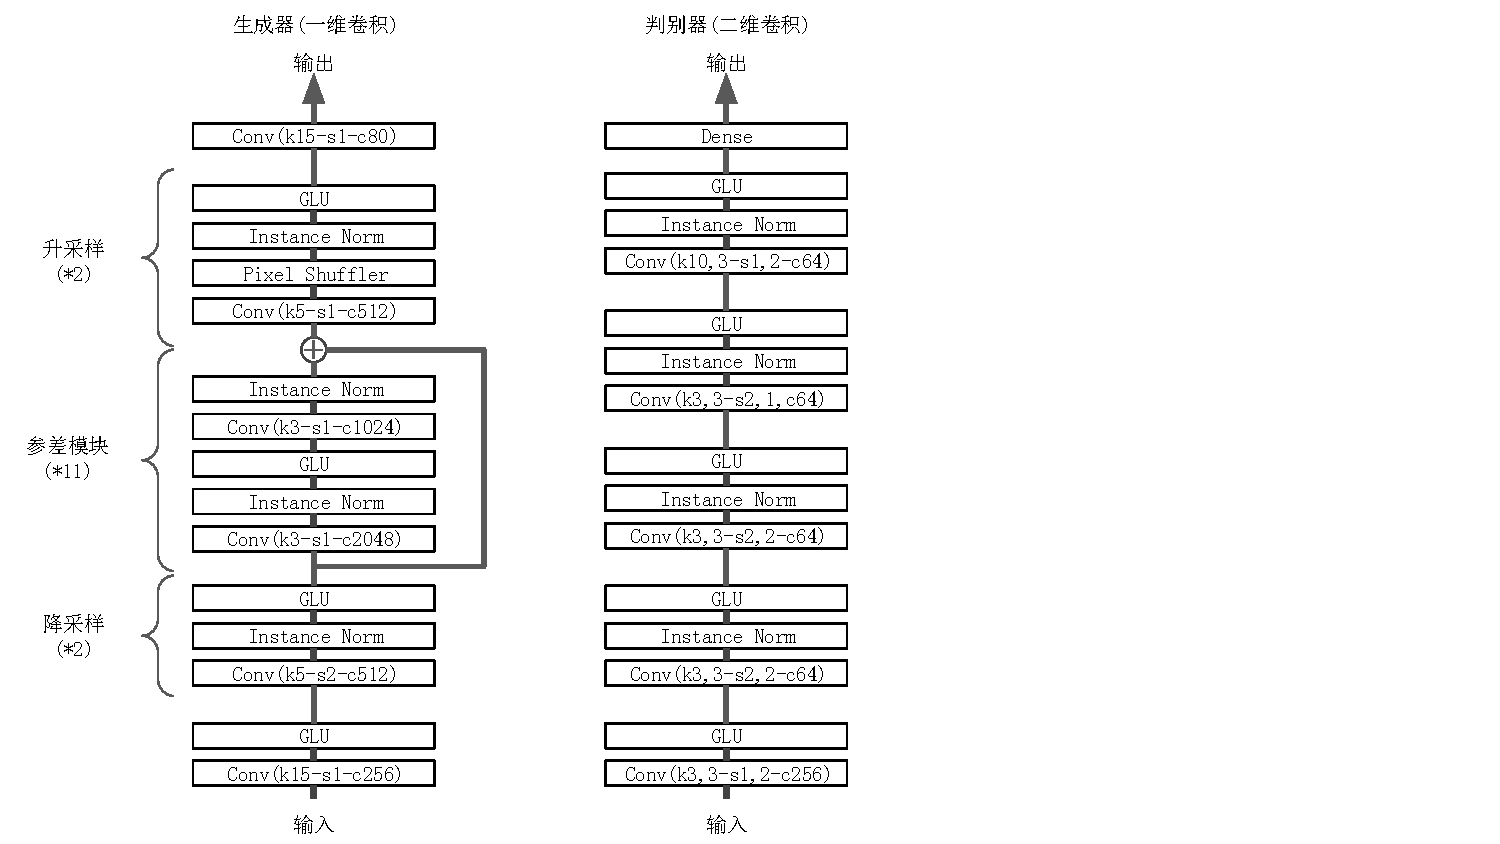
\includegraphics[width=12cm,trim=0 0 250 0,clip]{figure/4_networks.pdf}
    \bicaption[半优化CycleGAN网络结构图]
    {半优化CycleGAN网络结构图}
    {Architecture of the Semi-optimized CycleGAN}
    \label{fig:networks}
\end{figure}

我们在中文语音转换任务上评估了半优化CycleGAN和基频辅助特征的效果。所使用的中文数据集包含四个说话人,
两个男性说话人和两个女性说话人。所有训练和测试音频数据均录制于标准录音环境,且四个说话人都是以中文为母语的标准普通话说话人。
每个说话人的语音数据分为训练集、开发集和测试集,分别包含2000句,100句和20句,每句话音频长度在10s以内。
任意两个说话人的训练集数据均为非平行文本。音频采样率为16k。实验中特征首先通过WORLD声码器提取513维的频谱特征,513维的非周期信息和1维的基频特征,
之后用librosa\cite{mcfee2015librosa}和pysptk\cite{yamamoto2019r9y9}工具包提取80维的梅尔频谱特征和24维的梅尔倒谱特征。
帧移为5ms。注意到Tacotron2和平行语音转换任务中都使用了12.5ms帧移提取特征。然而在我们的实验中,
12.5ms的帧移会导致发音不完全或音素缺失的现象出现。我们因此使用5ms帧移来使用更细的频谱粒度来解决该问题。
虽然5ms的音质相比12.5ms相对较差,但是发音不完全的问题相比音质的下降更为严重。

首先使用每个说话人的训练数据各训练一个说话人相关的WaveNet声码器。其中WaveNet模型包含4个神经网络模块,
每个模块有6层神经网络。残差连接和门控层的隐层节点数为512,输出层的隐层节点数为256。
我们使用10个逻辑分布的混合逻辑分布来预测样本点分布。对于半优化CycleGAN,我们的模型结构如图~\ref{fig:networks}所示,
相比标准CycleGAN的网络结构,我们根据声学特征的帧移和维度对结构进行了调整:我们将生成器中残差模块的数量和卷积层的通道数乘2,
同时为了平衡生成器和判别器的对抗训练,判别器中四个降采样层的通道数都修改为64。
图中卷积层的标识k,s,c分别代表卷积核 (kernel) ,步长 (stride) 和频道数 (channel) 。生成器我们使用的是一维卷积,因为一维卷积
在抓取特征维度的总体关系的同时,更能够学习到特征的动态变化,因此在语音转换的任务中常使用一维卷积作为转换网络;然而在语音的后处理
任务 (Postfilter) 中,二维卷积更为常用,因为其更适合在改变特征形状的同时保留特征的原始结构,因此判别器使用二维卷积构建。
网络中Instance Normalization (IN) 是一种归一化方法,常用于风格迁移的任务中,其与常见的Batch Normalization (BN) 有所区别。
BN注重对每个batch进行归一化,保证数据的分布一致,因为判别模型中结果取决于数据的整体分布。但是在风格迁移的任务中,生成结果主要
依赖于具体的每个实例,所以对整体进行归一化并不适合用在风格迁移中,因此IN是对输入的高(Height)和宽(Width)进行归一化。由于IN的
训练和测试情况相同,不存在BN的不一致问题,因此也没有需要更新的参数。计算公式如下

\begin{equation}
    y_{bchw} = \frac{x_{bchw}-\mu_{bc}}{\sqrt{\sigma^2_{bc}+\epsilon}} * \gamma + \beta
\end{equation}

其中bchw分别代表特征的四个维度:batch,channel,height,width。$x$和$y$分别为输入和输出。$\gamma$和$\beta$是超参数。
$\mu_{bc}$和$\sigma^2_{bc}$计算方式如下

\begin{align}
    \mu_{bc} & = \frac{1}{HW}\sum^W_{w=1}\sum^H_{h=1}x_{bchw} \\
    \sigma^2_{bc} & = \frac{1}{HW}\sum^W_{w=1}\sum^H_{h=1}(x_{bchw}-\mu_{bc})^2
\end{align}

Pixel Shuffler是一种卷积网络中的升采样方法,其通过对特征矩阵进行变换和转置操作,将特征图的形状由$(B,f_1 * f_2 * C,H,W)$
转变为$(B,C,f_1 *H,f_2 *W)$。

数据载入部分我们使用了与CycleGAN-VC相同的策略,即在训练数据中随机截取连续128帧的特征片段。
所有网络都使用Adam优化器进行训练。训练batch大小设置为4。生成器和判别器的初始学习率分别为0.01和0.005,
不使用任何学习率调节策略。模型共训练350k步,身份损失只参与训练开始的前10k步。同时为了增强模型的鲁棒性,
在预测时,会将原始声学特征序列拆分为重叠的128帧片段,然后依次输入生成器,将生成的每个片段的中间部分提取出来,将他们拼接成最终的转换特征序列。

\subsection{客观评测}
本文首先采用梅尔频谱距离 (Mel-spectrogram Distorsion, Msd) 来判断转换模型在测试集上对特征转换的接近程度。
由于CycleGAN对抗学习的特性,其训练过程往往是不稳定的,模型性能与训练时长并不成正比关系。
因此我们记录了训练阶段模型在测试集上的梅尔频谱距离,频谱距离的计算使用了平行的测试数据,
这些数据不会参与模型训练。计算距离前会先用DTW算法对特征序列长度进行对齐。
我们在跨性别实验上对比了半优化CycleGAN和标准CycleGAN。实验结果如图~\ref{fig:msd}所示。
我们可以发现半优化CycleGAN所转换的梅尔频谱更接近目标特征,并且半优化CycleGAN的收敛曲线更为平稳。在实际实验中,
半优化CycleGAN也更容易训练和优化。

\begin{figure}[!hbtp]
    \centering
    \bisubcaptionbox{男性说话人转女性说话人}%
                    {Male to female}%
                    [12cm]{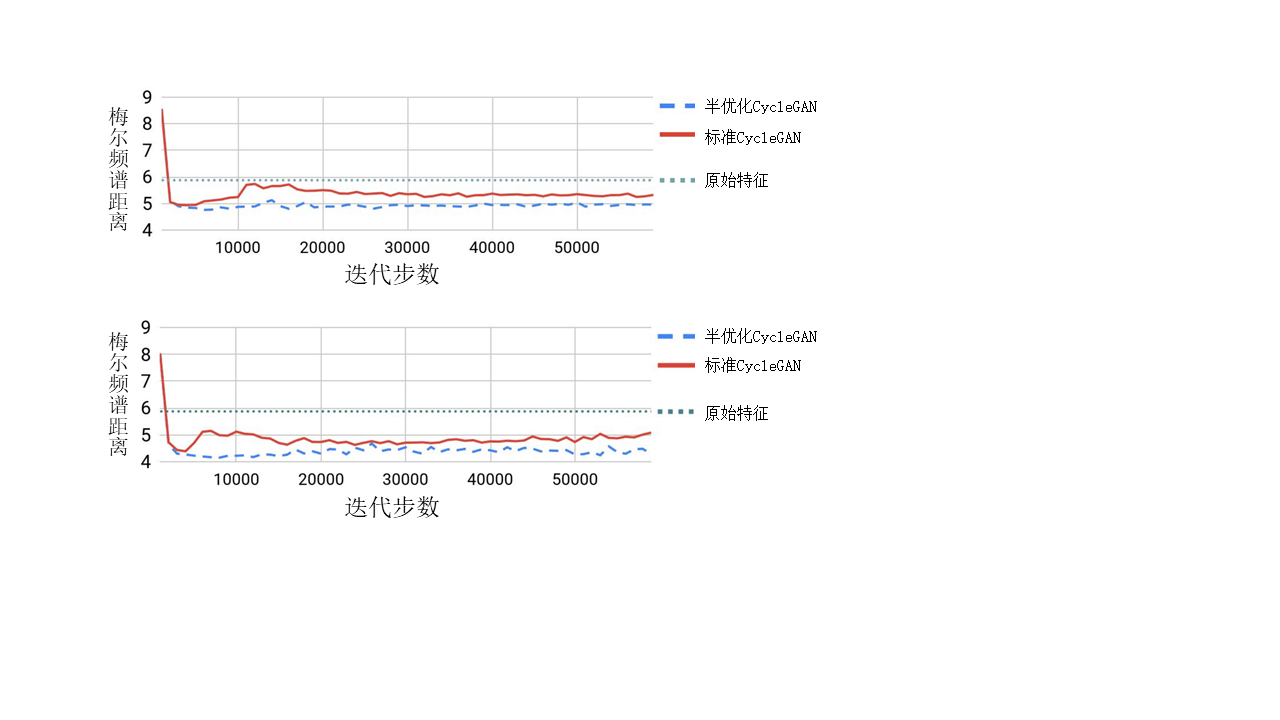
\includegraphics[width=12cm,trim=50 320 350 60,clip]{figure/4_msd.png}} \\
    \vspace{0.5cm}
    \bisubcaptionbox{女性说话人转男性说话人}%
                    {Female to male}%bisubcaptionbox
                    [12cm]{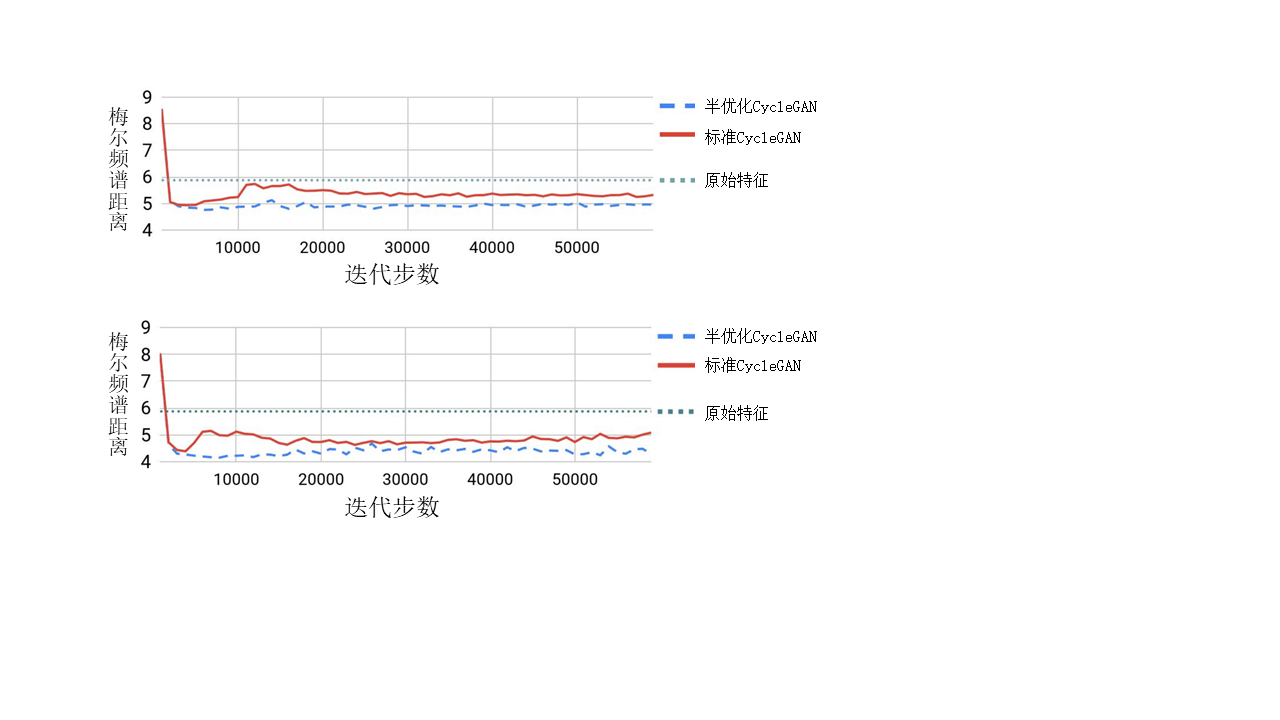
\includegraphics[width=12cm,trim=50 150 350 240,clip]{figure/4_msd.png}}
    \bicaption{标准CycleGAN和半优化CycleGAN在训练过程中梅尔频谱距离的对比}
              {Comparison of Msp distance between conventional CycleGAN and SoCycleGAN during training}
    \label{fig:msd}
  \end{figure}

为了验证基频转换的效果,在平行测试集上分别用WORLD声码器从转换音频和目标音频中提取基频特征,
统计各自的基频分布以及对齐后的标准误差。如表~\ref{tab:mse}所示,其中Source,Target分别代表原始真实特征
和目标真实特征,Linear代表线性变换的基频特征,Proposed w/o LF0代表没有使用基频辅助特征转换的基频,
Proposed代表使用了基频辅助特征后转换的基频。可以发现相比于线性变换,
基频辅助特征所转换的基频误差有较为明显的降低,同时基频分布也较接近目标的基频分布。
我们认为这是因为:(1)梅尔频谱可以实现基频的隐式转换,从而可以对基频进行比线性变换更复杂的变换映射;
(2)辅助特征通过引入显示的基频特征,可以帮助模型学习梅尔频谱中和基频信息高度相关的隐含表示,
进而提升基频的转换能力。

\begin{table} 
    \centering 
    \bicaption{转换基频和目标基频之间误差、均值和方差的对比}{Comparison of MSE, mean and standard deviation between target and converted F0}

    \begin{subtable}[t]{0.9\textwidth}
        \centering
        \bicaption{女性说话人转男性说话人}{Female to male}
        \begin{tabular}[t]{ cccc }
            \toprule
            % \hline
            %\multirow{1}{*}{Methods} & \multicolumn{3}{|c|}{Female to male} \\
             %\cline{2-4}
            Methods  & RMSE (Hz) & Mean (Hz) & Std (Hz) \\
             %\hline
             %\hline
            \midrule
            Target                  & 0 & 133.25 & 34.72             \\
            \midrule
            %\hline
            %\hline
            Source                    & 65.12 & 236.11 & 55.00            \\
            %\hline
            Linear                       & 17.13 & 127.10 & 28.58               \\
            %\hline
            Proposed w/o LF0                       & 17.44 & 124.66 & 27.74            \\
            %\hline
            Proposed                       & \textbf{16.69} & 126.31 & \textbf{29.82}   \\
            %\hline
            \bottomrule
            \end{tabular} 
        \label{tab:f0f2m}
    \end{subtable}
    \bigskip
    \vspace{1mm}
    \quad
    \begin{subtable}[t]{0.9\textwidth}
        \centering
        \bicaption{男性说话人转女性说话人}{Male to female}
        \begin{tabular}[t]{ cccc }
            \toprule
            %\hline
            %\multirow{2}*{Methods} & \multicolumn{3}{|c|}{Male to female}\\
             %\cline{2-4}
             Methods & RMSE(Hz) & Mean (Hz) & Std (Hz) \\
             %\hline
             %\hline
            \midrule
            Target                   & 0 & 236.11 & 55.00            \\
            \midrule
            %\hline
            %\hline
            Source                        & 67.10 & 133.25 & 34.72            \\
            %\hline
            Linear                     & 34.13 & 248.04 & 67.04              \\
            %\hline
            Proposed w/o LF0                   & 32.51 & 254.71 & 59.53              \\
            %\hline
            Proposed                      & \textbf{30.37} & 248.66 & \textbf{58.92}   \\
            %\hline
            \bottomrule
          \end{tabular}
        \label{tab:f0m2f}
    \end{subtable}

\label{tab:mse}
\end{table}  

\subsection{主观评测}
为了对系统的转换效果进行测试,我们采用较为普遍的主观听音测试来评测转换语音的质量。
所有的听音测试在同性别和跨性别上都进行了测试,并从测试集中随机选择了十句话让测试人员评测。
每一句话在每一次测试中被至少六个测试人员评价。不同系统的转换音频以随机顺序提供给测试人。
测试人皆是以普通话为母语的说话人。为了验证所提框架和改进的有效性,
我们使用模型消融测试 (Ablation test) 来比较不同系统。所比较的系统实验配置如下:

\begin{enumerate}
    \item N:真实语音
    \item Re:真实语音提取的梅尔频谱特征,用WaveNet合成
    \item B:标准CycleGAN预测的梅尔倒谱系数特征,用WORLD合成(基线系统,baseline)
    \item P:半优化CycleGAN预测的梅尔频谱特征,引入基频辅助特征,用WaveNet合成
    \item P w/o SoCycleGAN:标准CycleGAN预测的梅尔频谱特征,引入基频辅助特征,用WaveNet合成
    \item P w/o F0:半优化CycleGAN预测的梅尔频谱特征,无基频辅助特征,用WaveNet合成
\end{enumerate}

为了评测自然度,我们使用平均主观意见分 (Mean Opinion Score, MOS) 测试。
系统N和Re分别作为语音音质的上限分数和声码器的上限分数。
除此之外我们也测试了所提出的系统在小数据集上的表现,即在相同配置下100、200、500句话训练集的效果。
为了评测相似度,我们使用相同/不相同测试 (same/different test) 。

\begin{figure}[!htp]
    \centering
    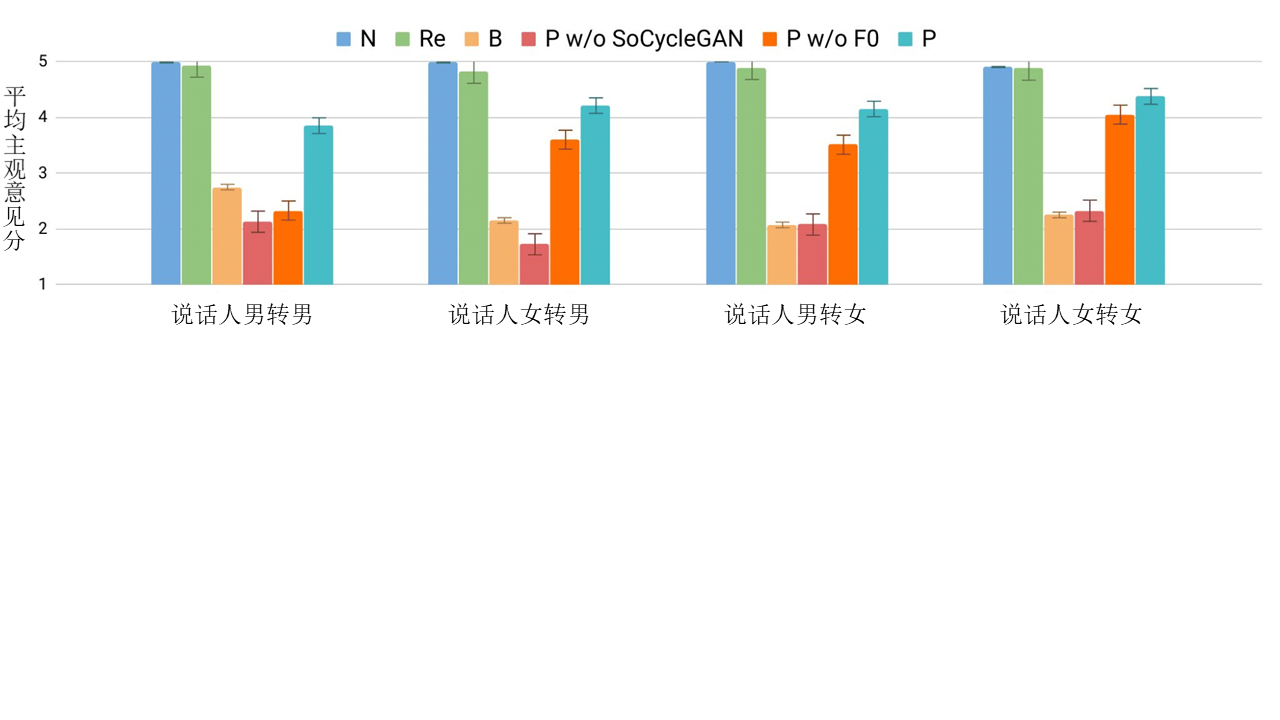
\includegraphics[width=13cm,trim=0 290 0 0,clip]{figure/4_mos.png}
    \bicaption[不同方法在语音自然度上的平均主观意见分对比图]
    {不同方法在语音自然度上的平均主观意见分对比图}
    {MOS comparison among different methods}
    \label{fig:mos}
\end{figure}

\begin{figure}[!htp]
    \centering
    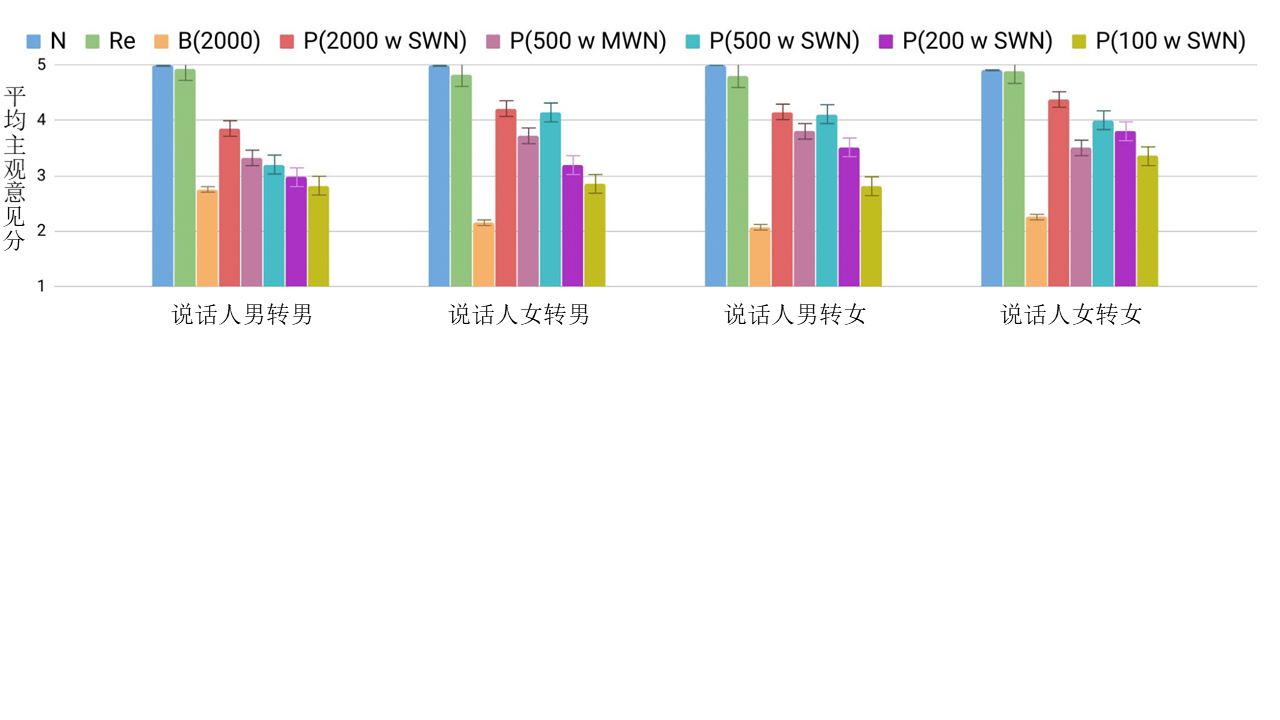
\includegraphics[width=13cm,trim=0 290 0 20,clip]{figure/4_mosdata.png}
    \bicaption[不同大小训练数据集在语音自然度上的平均主观意见分对比图]
    {不同大小训练数据集在语音自然度上的平均主观意见分对比图}
    {MOS comparison among different training data set}
    \label{fig:mosdata}
\end{figure}


图~\ref{fig:mos}展示了MOS测试的结果。对比系统P和P w/o SoCycleGAN,可以看到半优化CycleGAN在自然度上的提升。
从P和P w/o F0的对比,也能发现基频辅助特征的提升,
尤其在男性到男性的实验中(在该实验中音调错误问题最为严重)。
图~\ref{fig:mosdata}展示了所提出系统在不同训练数据量下的性能对比。2000,500,200和100分别代表训练数据集的大小。
SWN代表单说话人WaveNet,是由2000句特定说话人的训练集训练而成,
用以测试半优化CycleGAN的上界。MWN代表多说话人的WaveNet,是由十个中文说话人十几小时数据训练而成。
可以发现提出的系统在至少500句的训练集上可以生成较高音质的转换音频。
注意到我们对于小数据集没有对模型结构进行调整,因此在音质上仍有提升的空间。
相似度实验的结果在图~\ref{fig:sim}展示,可以发现所提出的框架在四个说话人对上都有更好的相似度表现。


\begin{figure}[!htp]
    \centering
    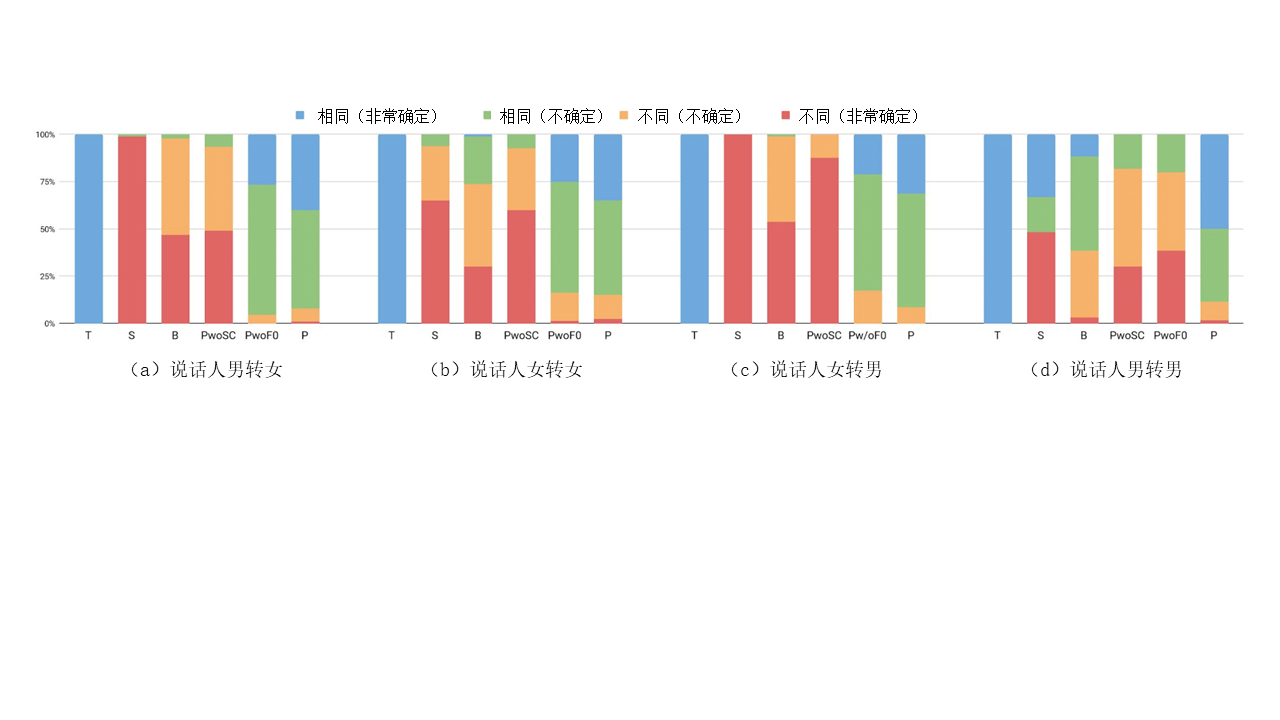
\includegraphics[width=14cm,trim=25 250 40 60,clip]{figure/4_sim.png}
    \bicaption[不同系统在四个说话人对上的相似度对比图]
    {不同系统在四个说话人对上的相似度对比图}
    {Comparison of similarity to target speaker in four speaker pairs}
    \label{fig:sim}
\end{figure}

\section{本章小结}

本章介绍了一种高音质的非平行语音转换框架,针对标准CycleGAN-VC存在的两个问题,
本章提出半优化CycleGAN和基频辅助特征,
并说明了这两个结构可以在基于梅尔频谱的WaveNet声码器下生成高音质的转换语音。
对比标准CycleGAN,半优化CycleGAN对语音自然度和相似度有着较为明显的提升。
基频辅助特征的引入同样也帮助模型更好地从梅尔频谱中学习到基频信息的表示和转换。
主观评测和客观评测表示,
所提出的系统表现优于标准CycleGAN和WORLD声码器的系统和标准CycleGAN和WaveNet声码器的系统。
下一章将介绍该框架在难度更大的语音转换任务:跨语种转换任务上的优化。


\chapter{基于说话人特征的跨语种语音转换优化方法}

\section{引言}

上文介绍了本文提出了基于半优化CycleGAN的非平行语料语音转换系统,该框架可以在一般非平行语料的语音转换任务上
得到较高的音质。然而,当原始说话人和目标说话人两个领域的差距较大时,转换的难度就会显著增加,差距可以体现在
说话人信息,语速,语义,音调等。在这种情况下,转换语音的音质会有明显的下降,甚至会无法训练。另一方面,实际
应用场景中,两个差距较大的领域是比较常见的,之前实验中的数据都是在专业录音环境下录制的平稳朗读语音,属于较为
理想的情况。因此,对领域差距较大情况下的语音转换任务进行优化具有较高的实际应用价值和研究价值。本章将对其中
较为极端的任务作为研究对象,即跨语种的语音转换。在该任务中,两个领域不仅是说话人信息不同,在语义信息上也
具有较大的差异,这对模型性能提出了挑战。

本章提出一种基于说话人特征的跨语种语音转换方法,以第三章介绍的CycleGAN-VC方法为基础,在CycleGAN模型中引入
说话人识别机制。首先需要先训练一个说话人识别模型,之后使用模型中的d-vector提取器来作为CycleGAN中判别器的
前置模型,使得判别器可以只使用说话人信息作为判别标准。实验证明,引入说话人特征的语音转换方法可以有效实现
在保留语义的前提下实现说话人语音转换,有效提升模型性能。

在接下来的内容中,将首先对跨语种语音转换和相关工作进行简要介绍,然后对说话人识别及其相关特征进行说明,
之后将详细介绍本章提出的引入说话人特征的跨语种语音转换优化方法,最后对实验配置及其结果进行分析。

\section{跨语种语音转换}
\subsection{跨语种语音转换概述}
根据转换语言条件的不同,可以将语音转换分为两类:单语种语音转换和跨语种语音转换。在单语种语音转换中,训练集中
原始说话人和目标说话人的语言是相同的,在测试时也是同一种语言。相对的,跨语种语音转换则是原始说话人和目标说话人的
语言不同,在此基础上可以将其再分为两类:一类是原始说话人的训练集是双语种的,其中一个语种和目标说话人一致;另一类
则是完全不相同。早期在跨语种语音转换上的研究多基于第一类情况,在本章我们则将以第二类为研究对象。跨语种语音转换具有较好
的发展和应用前景,作为无监督学习任务,其可以实现让一个不会说某种语言的说话人以他的声音说该语言。在语音翻译中,
通常需要将某个说话人的语音翻译为另一种语言的语音,然而翻译语音通常不是该说话人的声音,跨语种语音转换便可以作为
补充,完善语音翻译的整个环节。

尽管跨语种的语音转换的研究仍处于初步阶段,但研究人员针对跨语种的特点,提出了一些有效的方法。在\cite{AbeStatistical}中,
一个双语种的转换模型在目标语言的平行训练数据上训练,这需要原始说话人的训练数据不仅包含原始语种,也包含目标语种。
然而,事实上双语种说话人的双语数据是较难获得的。因此一些用于在非平行数据中找到对应的原始-目标帧的非平行对齐技术
被开发出来,例如单元选择\cite{sundermann2006text,Hao2015AA}和迭代对齐法\cite{erro2007frame,erro2009inca}。
但是这些方法由于不准确性使得转换性能只处于中等。基于声道长度归一化的音素映射方法也被提出\cite{sundermann2003vtln,qian2011frame},
这些方法中弯折函数是通过原始和目标特征之间最接近的音素或声学类来估计的。研究人员也提出了基于音素后验概率图的方法\cite{sun2016personalized,zhou2019cross},
该方法使用单语种或双语种的音素字典来作为中间的说话人无关特征,实现跨语种的转换。

\subsection{跨语种语音转换的难点}
% 1.不同语种之间文本信息不一致导致较难匹配
% 2.不同语种声学特征差异较大,对cyclegan有挑战性
如前文所述,跨语种语音转换作为一个无监督任务,是非平行语料语音转换的一个特殊任务。相比于通常的非平行语料语音转换,
跨语种语音转换转换难度更大,目前方法的效果也都不尽如人意。主要难度体现在以下两个方面。

\begin{figure}[!htp]
    \centering
    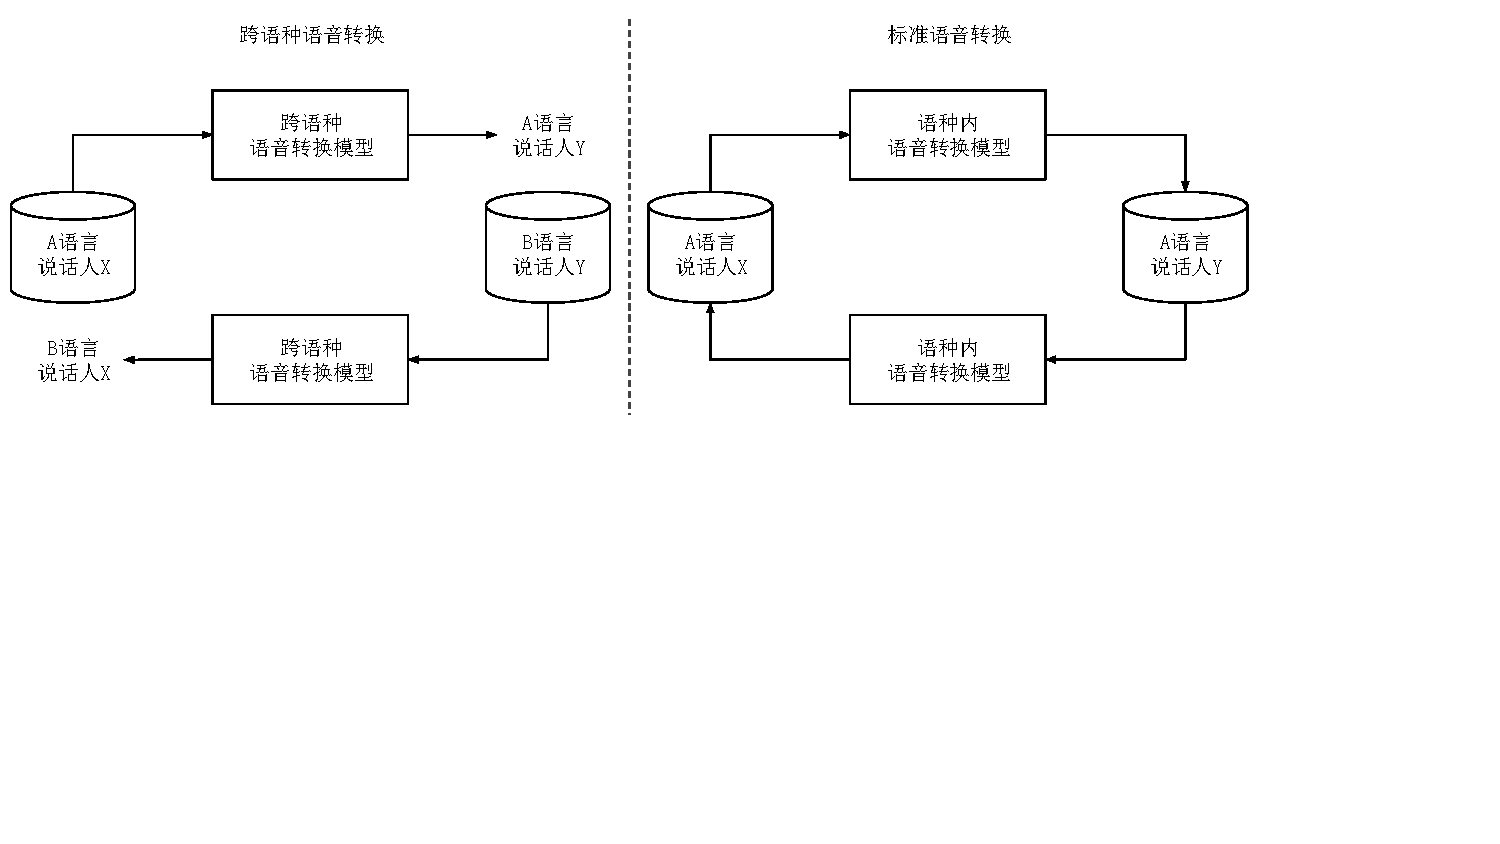
\includegraphics[width=14cm,trim=0 200 80 10,clip]{figure/5_clvc.pdf}
    \bicaption[跨语种语音转换和标准语音转换对比图]
    {跨语种语音转换和标准语音转换对比图}
    {Comparison of cross-lingual Voice Conversion and standard Voice Conversion}
    \label{fig:clvc}
\end{figure}

\begin{itemize}
    \item 不同语种之间文本信息不一致导致较难匹配。由于跨语种的语音转换涉及到两种不同的语言,因此平行语料的语音转换方法将完全不适用。
    另一方面若使用非平行的对齐方法,语种之间的巨大差异也会导致对齐准确度的下降。因此如何找到有效的单元匹配方式或无监督的训练方式是
    跨语种语音转换面临的主要挑战。
    \item 差异较大的声学特征与CycleGAN训练机制的矛盾。该矛盾分为两个方面。如前文所述,CycleGAN之所以能够实现语音转换任务,判别器在其中有着关键的作用。
    判别器在训练时,会分别输入正例和负例,对应训练标签$1$和$0$,其中正例是目标说话人的真实特征序列,负例是从原始说话人声学特征经
    生成器转换的目标说话人的转换特征序列,判别器的目标是尽可能地区分正例和负例。生成器在训练时会将生成的目标说话人转换特征传递给判别器,
    并将判别器的判别结果与$1$计算损失,来衡量转换特征和真实目标特征之间的差距,然后将梯度回传给生成器,这样生成器下次在遇到类似输入时,
    就会生成更接近判别器正例的转换特征。从图\ref{fig:clvc}中可以注意到,在跨语种语音转换中,判别器的正例
    是目标语种的目标说话人特征序列,而负例是原始语种的目标说话人特征序列。当判别器尝试区分正负例时,总是会尝试以区分度最大的信息作为
    判别要素,此时当语种信息的差异化大于说话人信息的差异化时,判别器就会转变为一个语种分类器,进而导致生成器无法从判别器中得到正确的
    梯度,因此在基线试验中,经常会导致模型在训练时无法训练成功:输入中文,生成器会输出无意义的英文语音。另一方面,语种的差异也会导致
    跨语种语音转换没有一个标准的对偶任务。如图\ref{fig:clvc}中左图所示,主任务为将说话人X的A语言转为说话人Y的A语言,理论上对偶任务
    应是说话人Y的A语言转为说话人X的A语言,而实际上对偶任务则是说话人Y的B语言转为说话人X的B语言。这样的不完全对偶性也增加了CycleGAN在
    跨语种语音转换任务上的难度。
\end{itemize}

\section{说话人识别}
\subsection{说话人识别概述}
说话人识别,也称声纹识别,同指纹识别,人脸识别相同,是一种新兴的生物特征识别技术。该技术从连续的语音信号中提取说话人相关的离散特征,
将说话人特征与数据库中的特征进行对比,得到匹配的说话人身份,从而实现对说话人身份的识别。说话人识别技术与语音识别技术都是输入语音信号
的分类任务。但不同的是,语音识别更专注于语音的说话内容,并尽量忽视掉说话人信息,而说话人识别则更注重语音的说话人是谁,而相对较少
关注语义信息。对于不同的说话人,其声道长度,声带基频,口腔及发音习惯等都有较大的区别,因而可以根据语音来判断说话人的身份,由于不同
发音人的语速,节奏也有区别,因此韵律信息也会被考虑。说话人识别通用框架主要包括两个部分,注册以及测试。注册是指用需要识别的说话人语音训练
识别模型,测试则是用训练好的模型对新来的语音进行识别。

根据实际应用场景的不同,说话人识别可以分为两类:说话人确认(Speaker Verification)和说话人辨认(Speaker Identification)。
其中说话人确认是针对某个特定说话人的识别,对于输入的语音,说话人确认模型输出是/否,代表该语音是否是该说话人
所说,属于二分类问题。说话人辨认则是对于输入的语音,在给定的说话人集合中,找出最符合的一个说话人,输出该语音是哪个说话人所说,
是多分类问题。说话人识别和说话人辨认主要在训练数据和输出层面有所区别,相比而言,说话人辨认在候选集合较大时,难度较高。
根据注册和测试时语音文本是否一致,可以将说话人识别分为文本相关(Text-dependent)的识别和文本无关(Text-independent)的说话人识别。
文本相关的说话人识别要求测试时提供的语音文本内容与训练时相同,模型在文本相同的先验下判断说话人身份,往往可以达到不错的性能。而文本无关的说话人识别则对
测试时的文本内容没有限制,使用环境也相对更自由,但建模难度也往往更大。说话人识别的应用非常广泛,包括声纹加密,语音检索,说话人核对,
和司法鉴定等。

在2012年以前,说话人识别的研究还主要以基于统计的机器学习方法为主,在2012年后以深度学习为基础的方法不断提出,如bottleneck feature、
d-vector、x-vector和j-vector等,一些最新的思想也被加入训练过程中,如基于注意力机制和learning to rank的算法等。
可以这些算法分为三类:基于i-vector的算法,基于DNN的算法和基于注意力机制和learning to rank等的改良算法。
其中基于DNN的算法中,早期用DNN以替代GMM计算后验概率,2014年Google提出的d-vector为标志\cite{variani2014deep},后续提出了一系列基于DNN的方法如
x-vector,j-vector等\cite{snyder2016deep,chen2015multi,shi2017double}。本文将采用基于d-vector的说话人识别技术,
将其应用到跨语种语音转换中。

\subsection{d-vector说话人特征}

\begin{figure}[!htp]
    \centering
    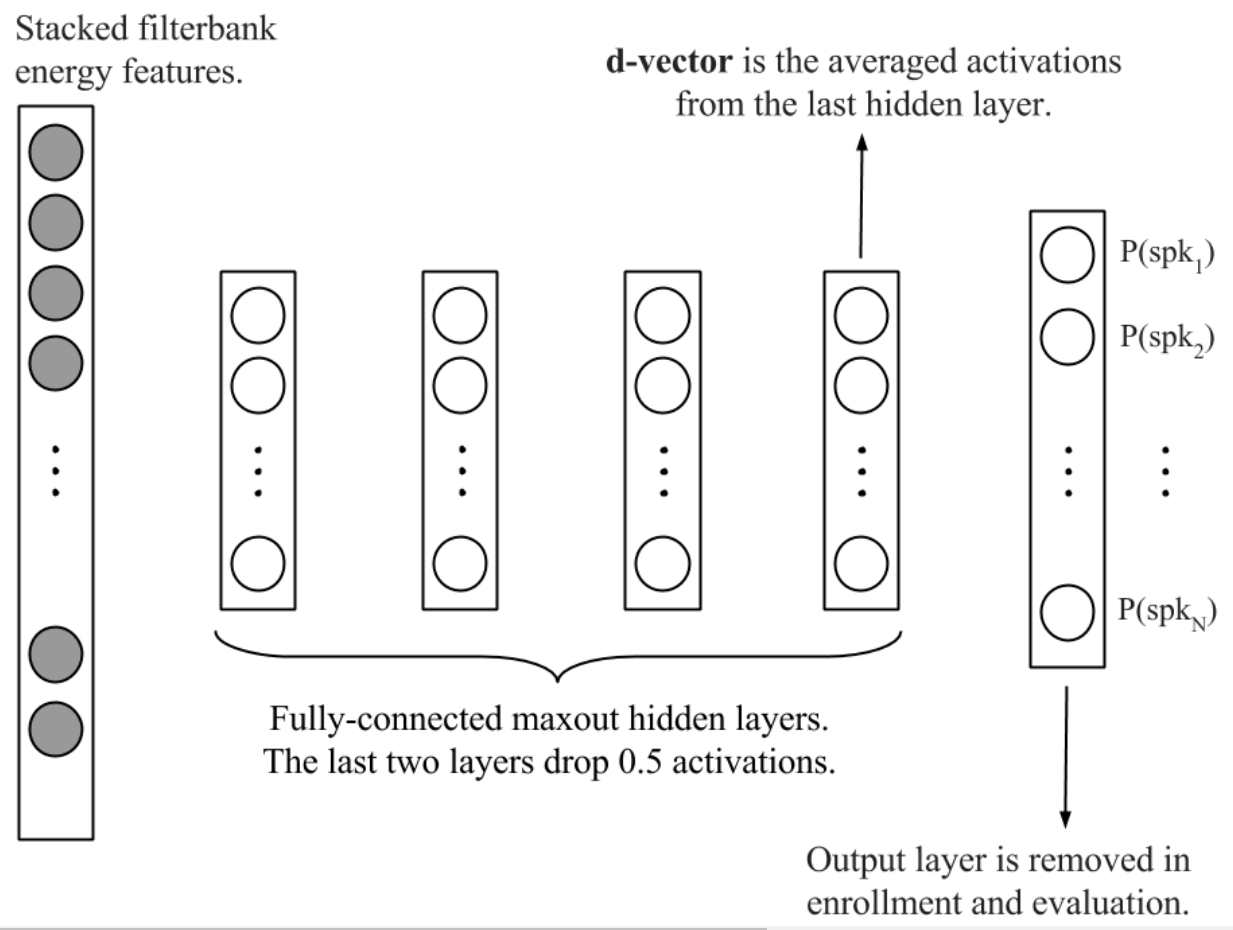
\includegraphics[width=10cm,trim=0 10 0 0,clip]{figure/5_dvector.png}
    \bicaption[基于DNN的说话人验证示意图\cite{variani2014deep}]
    {基于DNN的说话人验证示意图\cite{variani2014deep}}
    {Schematic diagram of the DNN model for speaker verification}
    \label{fig:dvector}
\end{figure}

基于d-vector的说话人特征提取模型如图~\ref{fig:dvector}如图所示。该方法和核心在于使用DNN网络作为一个说话人
特征提取器。在该目标下,首先在帧级别训练一个有监督的DNN模型。模型的输入是动态声学特征,即当前帧和前后若干帧的
拼接,目的是希望模型在判断时同时考虑一定范围内的上下文信息。模型的输出是一个向量,向量的长度取决于说话人的个数$N$。
训练时目标标签则是长度为$N$的one-hot向量,即除了输入特征对应的说话人序号在向量中的位置为1,其他值皆为0。

当DNN说话人识别模型训练完成后,即将DNN模型最后一个隐层的激励函数输出作为一个新的说话人表示(d-vector)。对于一句新的语音,
DNN对其中的每一帧都可以得到一个隐层向量,将所有帧的隐层向量累积起来,得到最终的说话人表示。这里选用最后一个隐层
的激励函数输出作为说话人表示而不是最终的$softmax$层,是因为输出层的长度是依赖于训练的说话人总数,无法根据具体
需要改变长短,而最后一个隐层则可以做到这点;另一方面,作者在实验中也发现最后一层隐层向量相比最终输出,其在没有见过
的说话人上有着更好的泛化性。d-vector的假设是认为训练好的DNN说话人识别模型,已经在最后一个隐层中学到了较为紧凑的说话人
表示,当训练时的说话人数目较多时,该表示也可以用来表达没有见过的说话人。

在测试阶段,给定一个特定说话人$s$的语音句集合$X_s = \left\{O_{s_{1}},O_{s_{2}},...,O_{s_{n}}\right\}$。
其中每个句子是一个观测集合$O_{s_{i}} = \left\{O_1,o_2,...,o_m\right\}$。首先对于每个观测,通过拼接上下帧得到其
动态特征,输入给训练好的DNN模型,获得对应的最后一层隐层向量输出,并将其归一化,作为该帧的d-vector。最终说话人$s$的表示则
是通过将所有的d-vector进行平均得到。当得到该说话人的一个新的语句时,将该句的d-vector与之前得到的说话人的最终表示计算
余弦距离,通过一个预先设定的阈值来得到最终的识别结果。

\section{引入说话人特征的跨语种语音转换}

\begin{figure}[!htp]
    \centering
    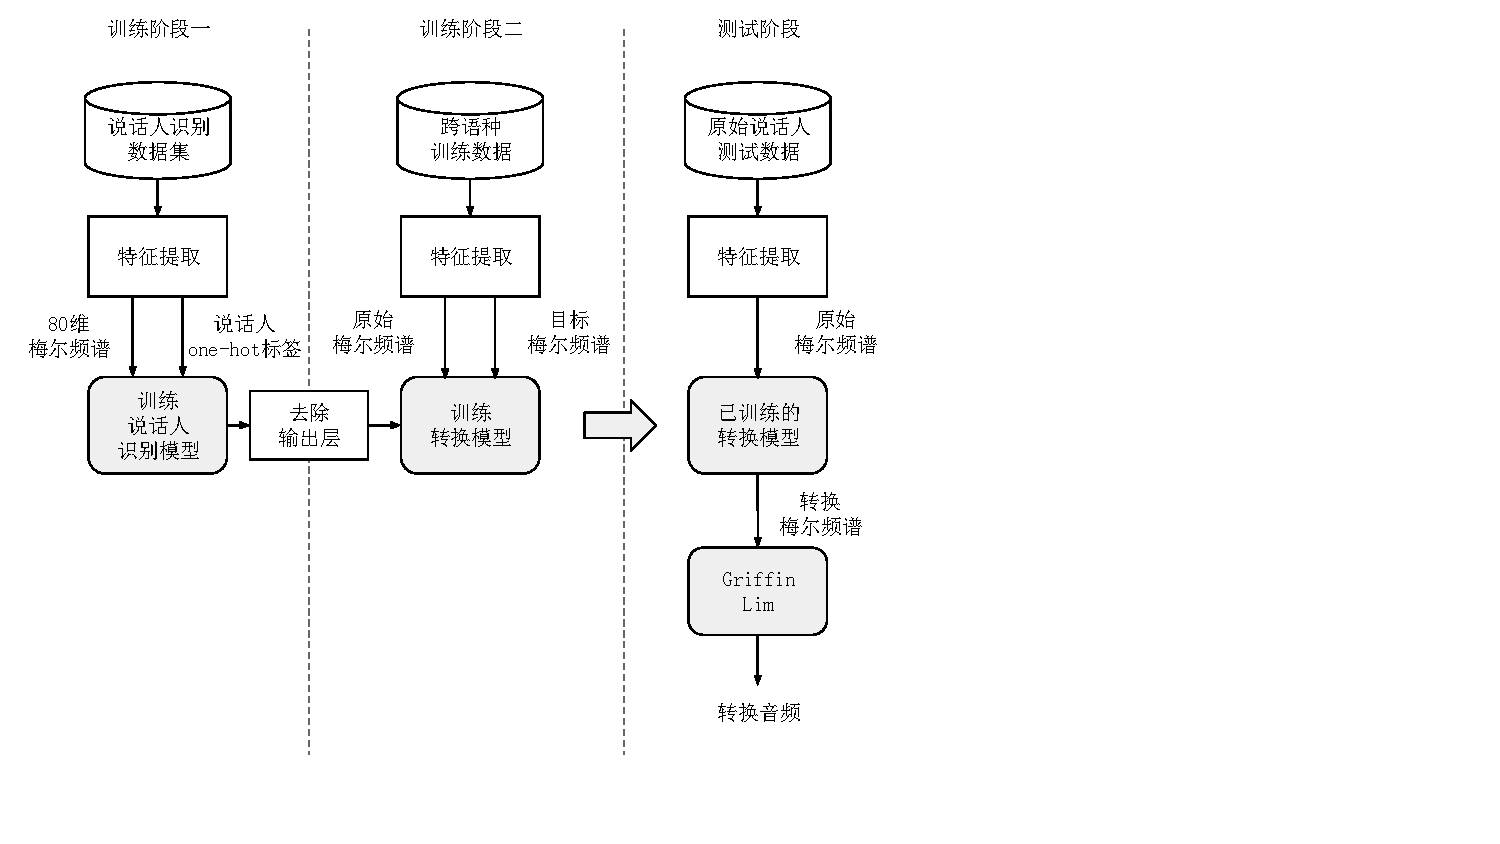
\includegraphics[width=12cm,trim=0 50 250 0,clip]{figure/5_proposedarch.pdf}
    \bicaption[引入d-vector的语音转换示意图]
    {引入d-vector的语音转换示意图}
    {Schematic diagram of the d-vector based Voice Conversion}
    \label{fig:5proposedarch}
\end{figure}

如图~\ref{fig:5proposedarch}所示,引入d-vector的跨语种语音转换方法分为三个阶段。在训练阶段一,一个语种无关的说话人识别模型在
专门用于说话人识别的数据集上进行训练,由于说话人识别模型将接入转换模型训练,为了与转换模型保持一致,
这里使用80维的梅尔频谱,并将对应的标签改为说话人的one-hot向量;在训练阶段二,将训练好的说话人识别模型去除输出层后,
作为说话人特征提取器加入转换模型中,在跨语种的语音转换数据集上进行特征提取和训练;测试阶段同通常的语音转换相同,先对测试的原始
语音提取特征,并传递给训练好的转换模型,得到模型输出的转换特征后使用Griffin Lim算法生成声音。
下文将详细介绍本文使用的语种无关的d-vector提取器和其与CycleGAN转换模型的结合。



\subsection{d-vector提取器和CycleGAN的结合}

\begin{figure}[!htp]
    \centering
    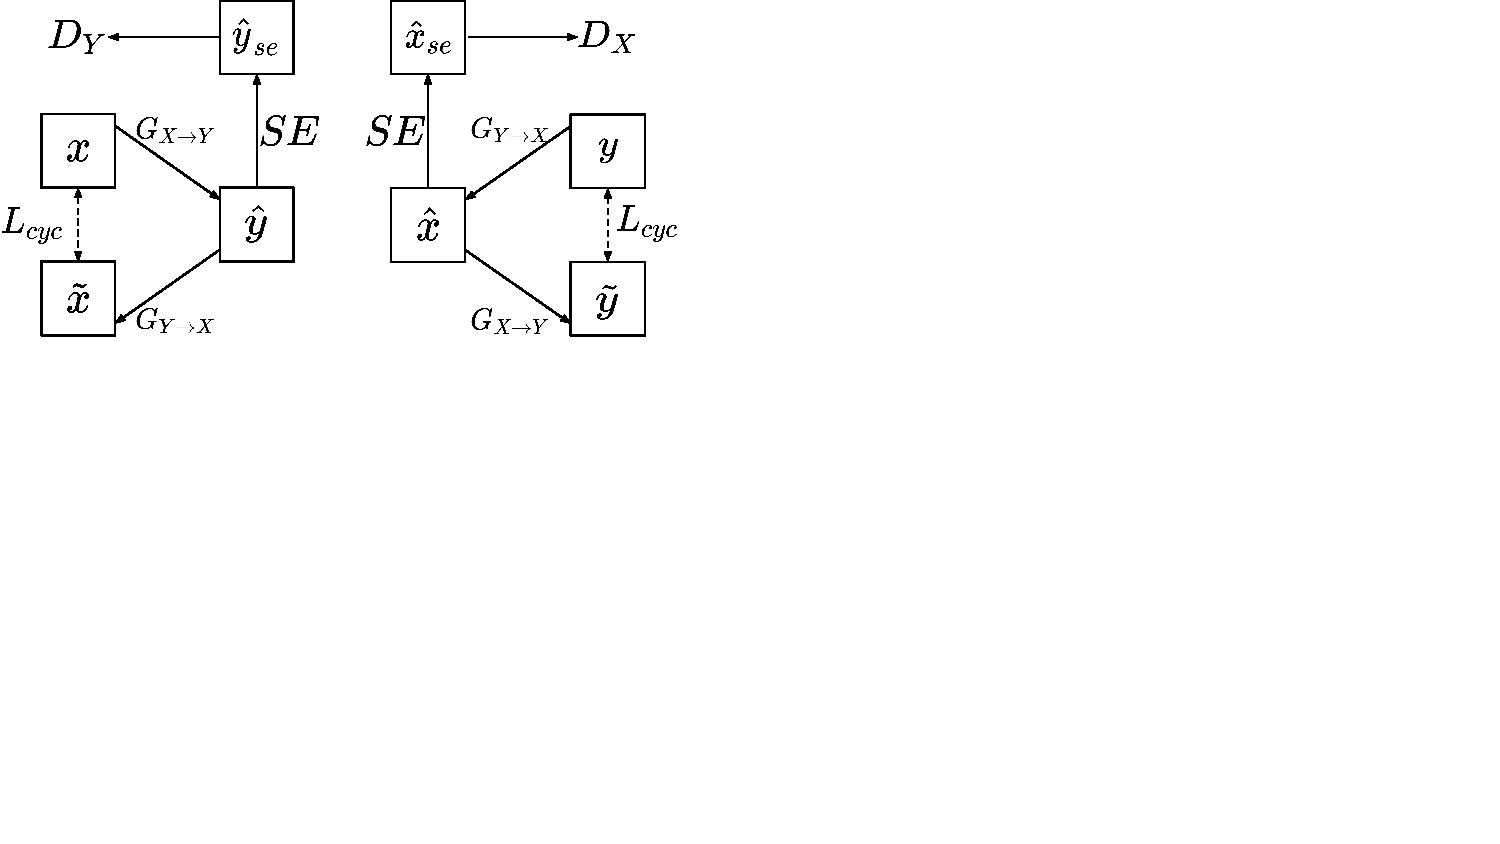
\includegraphics[width=8cm,trim=0 230 370 0,clip]{figure/5_dvectorcyclegan.pdf}
    \bicaption[基于d-vector提取器的CycleGAN模型示意图]
    {基于d-vector提取器的CycleGAN模型示意图}
    {Schematic diagram of the d-vector extractor based CycleGAN}
    \label{fig:dvectorcyclegan}
\end{figure}

如前文所述,跨语种的一大难点是差异较大的声学特征与CycleGAN训练机制的矛盾,其中主要矛盾是在CycleGAN模型
的训练过程中,判别器的正例和负例不仅在说话人信息上具有差异,由于语种的不同,在语义信息上也有着巨大的差异,
因此当语义信息的差异大于说话人信息的差异时,模型就会由说话人区分器变为语种区分器,极大降低了模型性能。
本章因此提出的引入说话人信息的语音转换方法,转换模型结构如图~\ref{fig:dvectorcyclegan}所示,其中$SE$
代表d-vector提取器,由预先训练好的语种无关的说话人分类器去掉输出层得到,$\hat{y}_{se}$是指由d-vector
提取器从转换特征和真实特征提取出的d-vector向量。可以看出,其与标准CycleGAN的最大不同是在判别器之前加入了
一个前置网络。该前置网络可以将声学特征向量中的说话人信息提取出来,进而在一定程度上忽略其中的语义信息。提取出来的
说话人表示再传递给对应的判别器,此时判别器只需要从说话人表示中判定真假,而可以在较大程度上减少语种信息对判别器的
影响。在整个模型的训练过程中,d-vector提取器只需要预先训练,之后就将参数固定,不再更新参数,只需要前向传播和
反向计算梯度,将判别器的梯度传递给生成器即可。此时对抗损失变为

\begin{align}
    L_{adv}(G_{X\rightarrow Y},D_Y) & =\mathbb{E}_{y\sim P_{Data}(y)}\left[log D_Y(SE(y))\right] \\
    & + \mathbb{E}_{x\sim P_{Data}(x)}\left[log(1-D_Y(SE(G_{X\rightarrow Y}(x))))\right] \\
    L_{adv}(G_{Y\rightarrow X},D_X) & =\mathbb{E}_{x\sim P_{Data}(x)}\left[log D_X(SE(x))\right] \\
    & + \mathbb{E}_{y\sim P_{Data}(y)}\left[log(1-D_X(SE(G_{Y\rightarrow X}(y))))\right]
\end{align}

$SE$在其中可以看成一个可以前向和反向传播的过滤模型,该模型输入声学特征,将其中的说话人之外的信息过滤掉,只留下
其中的说话人信息。这样判别器就可以在跨语种的数据集上实现类似同语种转换的效果。



\subsection{语种无关的d-vector提取器训练}


\begin{figure}[!htp]
    \centering
    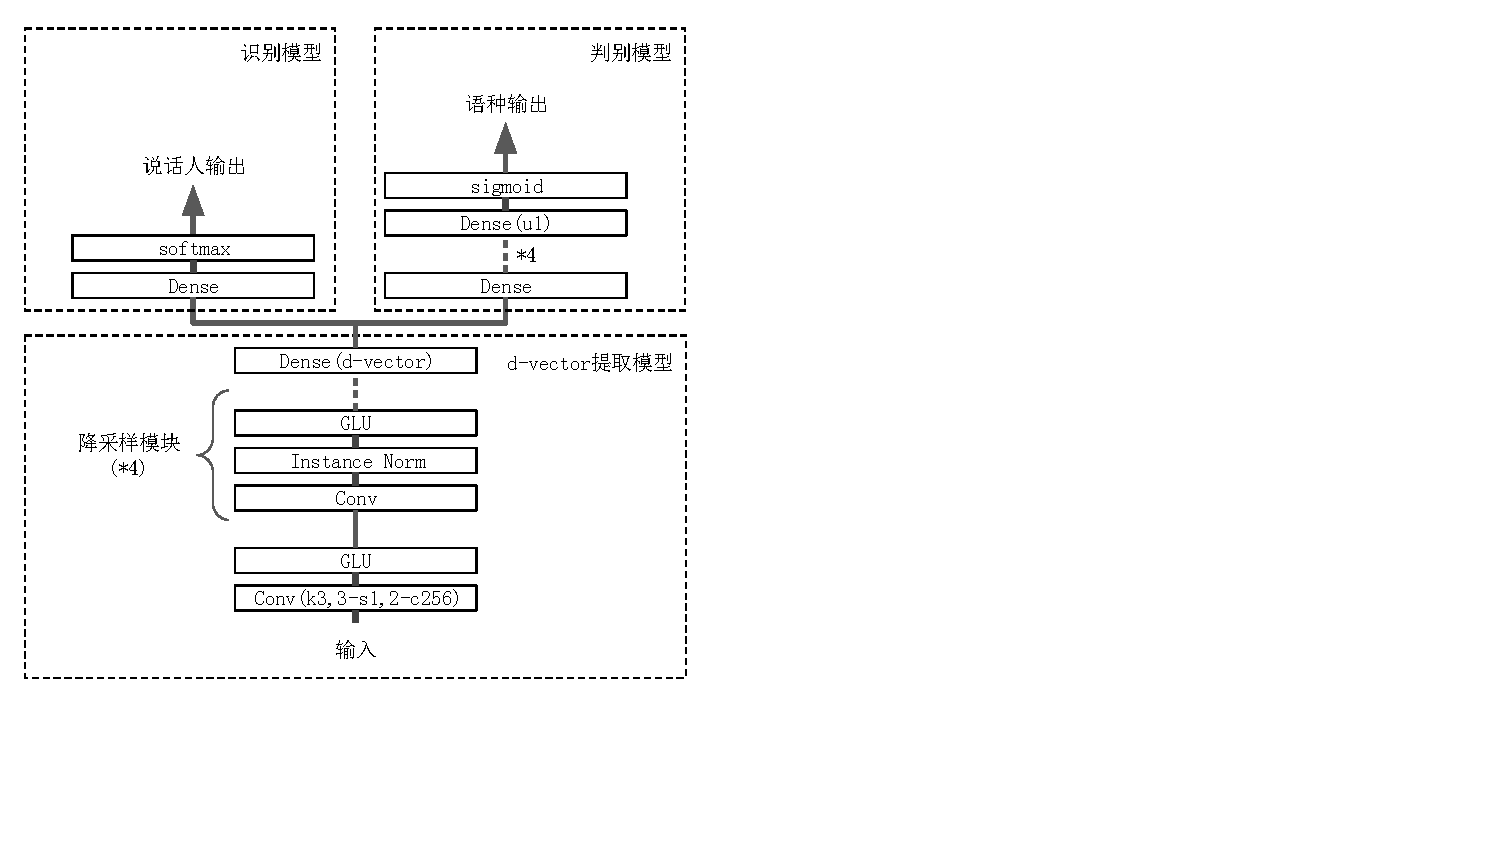
\includegraphics[width=10cm,trim=0 79 380 0,clip]{figure/5_d.pdf}
    \bicaption[说话人识别模型网络结构图]
    {说话人识别模型网络结构图}
    {Architecture of the speaker verification networks}
    \label{fig:5d}
\end{figure}

d-vector提取器作为判别器的前置网络,其功能从输入的声学特征序列中提取说话人表示,并尽可能地过滤掉特征中的语义语种信息。
对于训练一个标准的d-vector提取器来说,通常首先需要较多说话人的语料数据,每个说话人包含几句到几十句不等,目前常用的
开源数据中包括英文数据集voxceleb\cite{nagrani2017voxceleb}以及中文数据集CN-celeb\cite{fan2019cn}。不同于
通常的说话人识别任务,为了能够对原始语言的真实原始特征和目标语言的转换原始特征进行说话人信息上的判别,提取出的说话人表示
需要在中文和英文上尽可能一致。例如,使用英文数据集训练的d-vector提取器,如果测试时使用
数据集中一个说话人的中文语音,那么由于d-vector只见过英文,则提取出的说话人表示和这个说话人英文语音的表示很可能有较大差别。
即使d-vector在训练时见过两种语言,也不能认为这样训练出来的提取器不会考虑语种信息,这就陷入了同CycleGAN一样的问题。
解决该问题的方法有两种,一种是从数据角度入手,如果能够收集每个说话人都是双语或多语种说话人,可以收集到他们说不同的语种的语音
并且这样的说话人数据足够多的话,说话人识别模型则会将同一说话人的不同语种映射到同一个标签上,从而实现对语种的过滤。但这种方法通常
不可行,因为双语说话人的数据获取难度很大,更不用说很多个说话人了。因此本章提出另一种方法,即从对抗学习的角度来解决这个问题。

本章提出一种基于对抗学习的说话人识别网络结构。如图\ref{fig:5d}所示,该网络由三个部分组成,d-vector提取模型$V$,benjie
识别模型$C$和判别模型$D$构成。其中d-vector提取模型$V$负责从输入的声学特征中提取说话人表示,然后识别模型$C$从该说话人表示中
得到对应的说话人身份,另一方面说话人表示也传递给判别模型$D$,来输出对应的语种。这里d-vector提取模型$V$和判别模型$D$是对抗训练的,
即判别模型$D$的目标是尽可能地识别出d-vector属于哪个语种,而d-vector提取模型$V$则尽可能地生成无法判断语种的d-vector来欺骗判别模型$D$。
损失函数表示如下


\begin{align}
    L_{adv}(D) & =\mathbb{E}_{x\sim P_{Data}(x)}\left[log D(V(x))\right] \\
               & +\mathbb{E}_{y\sim P_{Data}(y)}\left[1-log D(V(x))\right]\\
    L_{adv}(V) & =\mathbb{E}_{x\sim P_{Data}(x)}\left[log (0.5-D(V(x)))\right] \\
               & +\mathbb{E}_{y\sim P_{Data}(y)}\left[log (0.5-D(V(y)))\right]
\end{align}

其中$x$和$y$分别为两个语种的训练数据。这里的对抗训练可以使用两种方法,一种是如公式所示d-vector提起器目标是生成让判别器无法判断的说话人表示,
即0.5,另一种方法则是在训练d-vector提取器时对判别器的损失传递负梯度,但这样可能会让d-vector中包含相反语种的信息,因此本章使用前一种方法来
训练说话人识别模型。

\section{实验分析}
本节对本章提出的引入说话人特征的跨语种语音转换方法的模型效果进行分析,将加入d-vector的语音转换模型与
标准CycleGAN进行对比,同时比较使用语种无关的对抗学习方法和不使用语种无关的对抗学习方法在跨语种语音转换任务上的性能区别。
主要通过主观实验和客观实验来验证d-vector的有效性及使用语种无关对抗学习方法对转换音质的影响。
% 客观指标可以用d-vector的距离来判断
% 引入说话人特征的有效性:
% 主观实验-自然度,相似度
% 系统:
% 1. baseline, 标准CycleGAN
% 3. 加入d-vector(d-vector 64, 100人)
% 4. 加入d-vector(d-vector 64, 1000人)
% 客观实验:
% 测试接上转换特征d-vector和目标特征的差距
% 1.d-vector提取器在clvc上的区分度,[dv 64 100;dv 64 500;dv 64 1000;]
% cycle-consistency loss
\subsection{实验配置}
本章实验所使用的数据集分为两种,在训练说话人识别模型时,本章使用了中文和英文的开源数据集CN-celeb和voxceleb。其中
voxceleb是一个视听数据集,包含1251个名人的超过100,000句语音,这些语音多是从上传到Youtube的采访视频中获取的。
CN-celeb是由清华大学发布的中文说话人识别开源数据集,该数据集包含1000个名人的超过130,000句语音。在训练转换模型时,
本章所使用的数据集包括一名男性的中文说话人(lcxinm),女性的中文说话人(gpyinf)和一名女性的英文说话人(ljspeech),
音频均为录制于标准环境的标准中英口语。且训练集和测试集分别为2000句和20句,每句话长度在10s以内。
语音转换任务通常分为同性别和跨性别,因此本章将英文说话人选
为原始说话人,将中文说话人选为目标说话人,分别训练女转女的同性别转换模型和女转男的跨性别转换模型。特征提取配置参考上一章。

本节所比较的系统实验配置如下:
\begin{itemize}
    \item N:真实语音
    \item CycleGAN:标准CycleGAN转换的梅尔频谱特征,用GL合成(Baseline)
    \item DV-CycleGAN:加入d-vector提取器的CycleGAN转换的梅尔频谱特征,用GL合成(D-Vector CycleGAN)
    \item LIDV-CycleGAN:加入语种无关的d-vector提取器的CycleGAN转换的梅尔频谱特征,用GL合成(Language Independent D-vector CycleGAN)
\end{itemize}

由于跨语种的语音转换无论在训练集还是测试集都没有平行语料,不存在真实的标签,因此很难通过频谱距离这样的客观指标来判断
特征转换的好坏。因此本章中客观实验将转换语音的d-vector与真实目标语音的d-vector进行对比来验证说话人相似度上的有效性,
同时通过转换模型训练时的重构损失来判断转换模型训练的好坏程度。
在主观实验中,本章将对自然度采用MOS打分的方式,对相似度采用ABX的偏好测试。

\subsection{客观实验}

为了验证d-vector在语音转换的有效性,本节首先对不同配置的d-vector提取器在语音转换任务的三个说话人上
进行可视化分析。本文根据训练说话人数目的不同和加入语种无关训练方式与否一共分为六个模型,每个模型对应图~\ref{fig:dvectordis}中
的一个子图,子图标题为模型的名称,100 speakers,500 speakers和1000 speakers分别代表训练集包含的说话人
数目,w/o adv和w/ adv分别代表不使用和使用语种无关的对抗训练方式。对于每一个模型,将三个说话人(lcxinm,gpyinf,ljspeech)的
20句测试集音频提取特征,模型对每一句分别计算一个d-vector,然后使用t-SNE算法\cite{maaten2008visualizing}对d-vector降到
二维空间,图中的每一个点代表一句话的d-vector。

% 1.d-vector在语音转换数据集上的分布

\begin{figure}[!ht]
    \centering
    \begin{minipage}[b]{0.9\linewidth}
        \centering
        \begin{subfigure}[b]{0.3\linewidth}
            \centering
            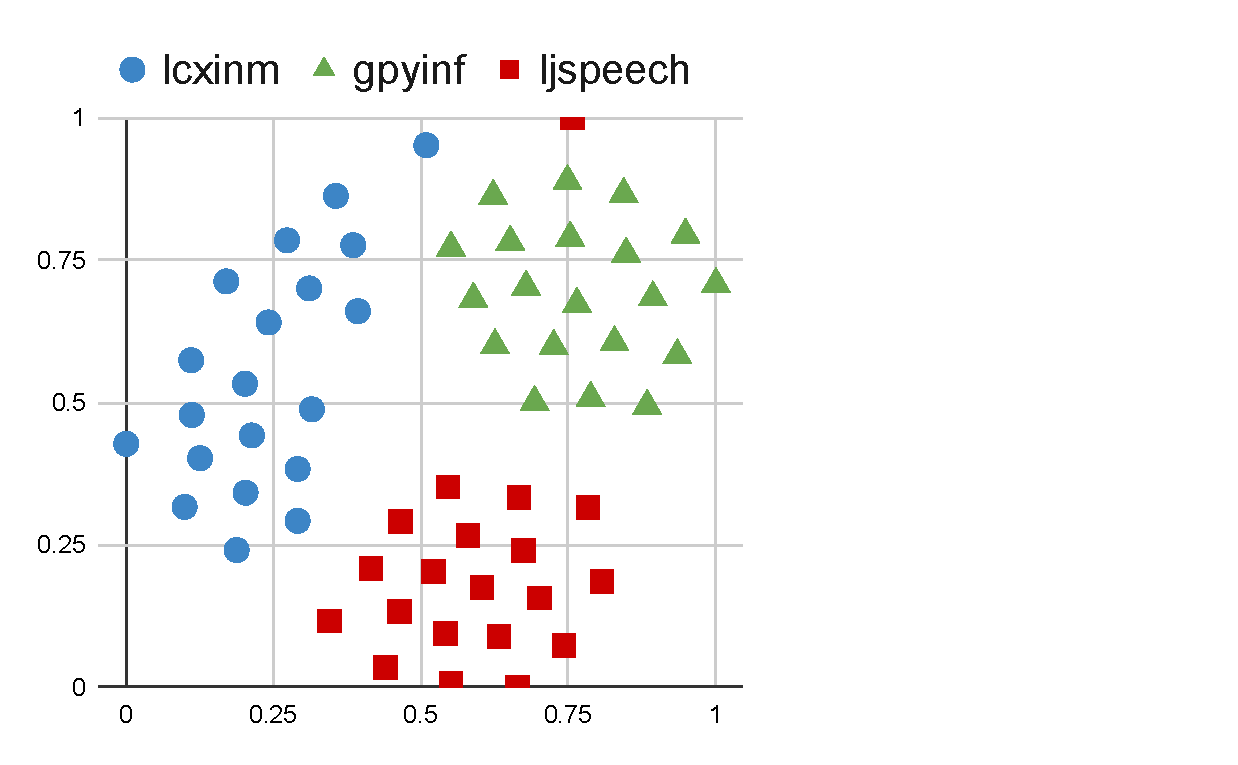
\includegraphics[width=\linewidth,trim=0 0 200 0,clip]{figure/5_dvector11.pdf}
            \caption{100 speakers w/o adv}
        \end{subfigure}        
        \begin{subfigure}[b]{0.3\linewidth}
            \centering
            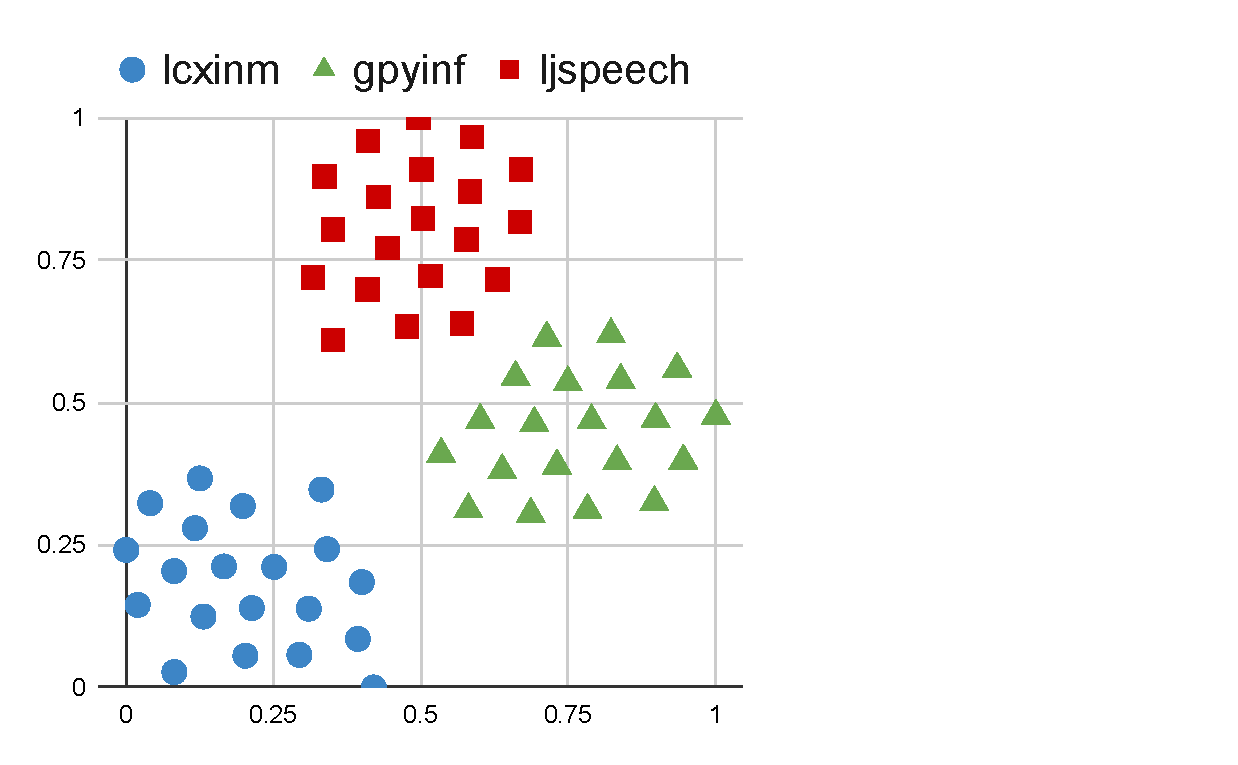
\includegraphics[width=\linewidth,trim=0 0 200 0,clip]{figure/5_dvector12.pdf}
            \caption{500 speakers w/o adv}
        \end{subfigure}   
        \begin{subfigure}[b]{0.3\linewidth}
            \centering
            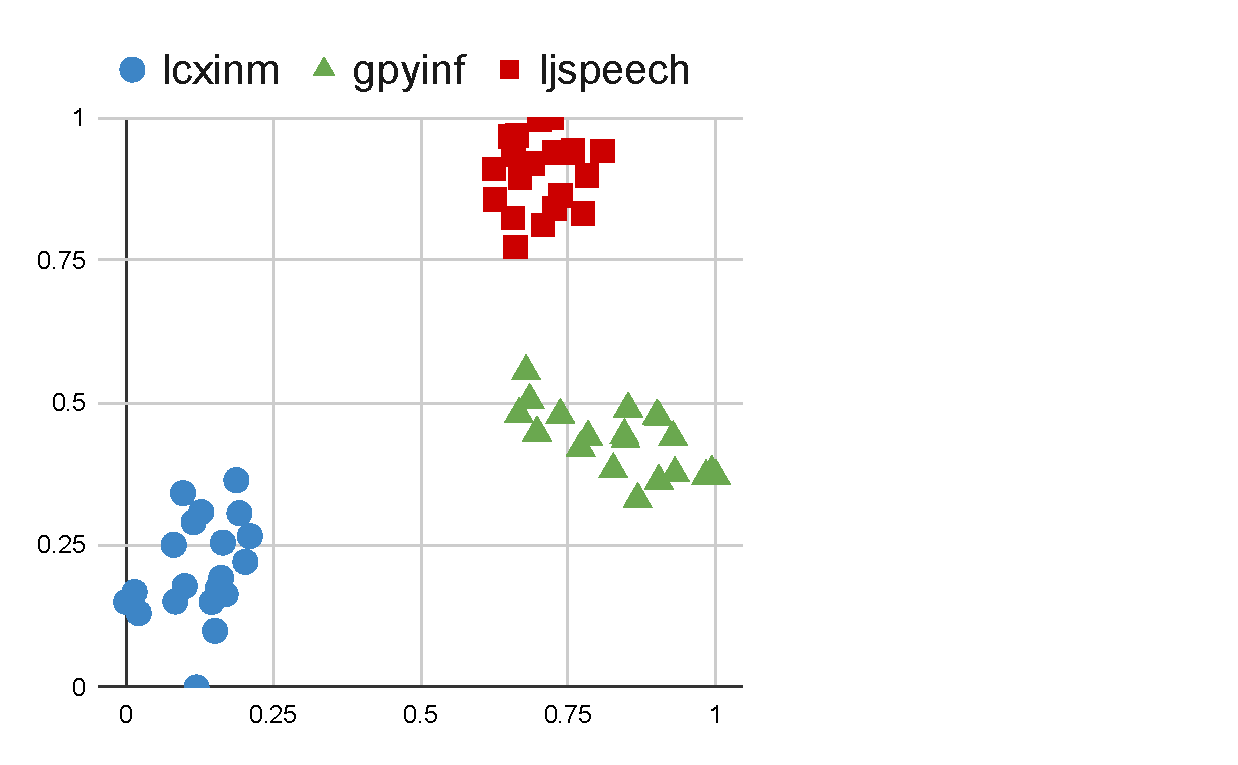
\includegraphics[width=\linewidth,trim=0 0 200 0,clip]{figure/5_dvector13.pdf}
            \caption{1000 speakers w/o adv}
        \end{subfigure}   
    \end{minipage}
    \begin{minipage}[b]{0.9\linewidth}
        \centering
        \begin{subfigure}[b]{0.3\linewidth}
            \centering
            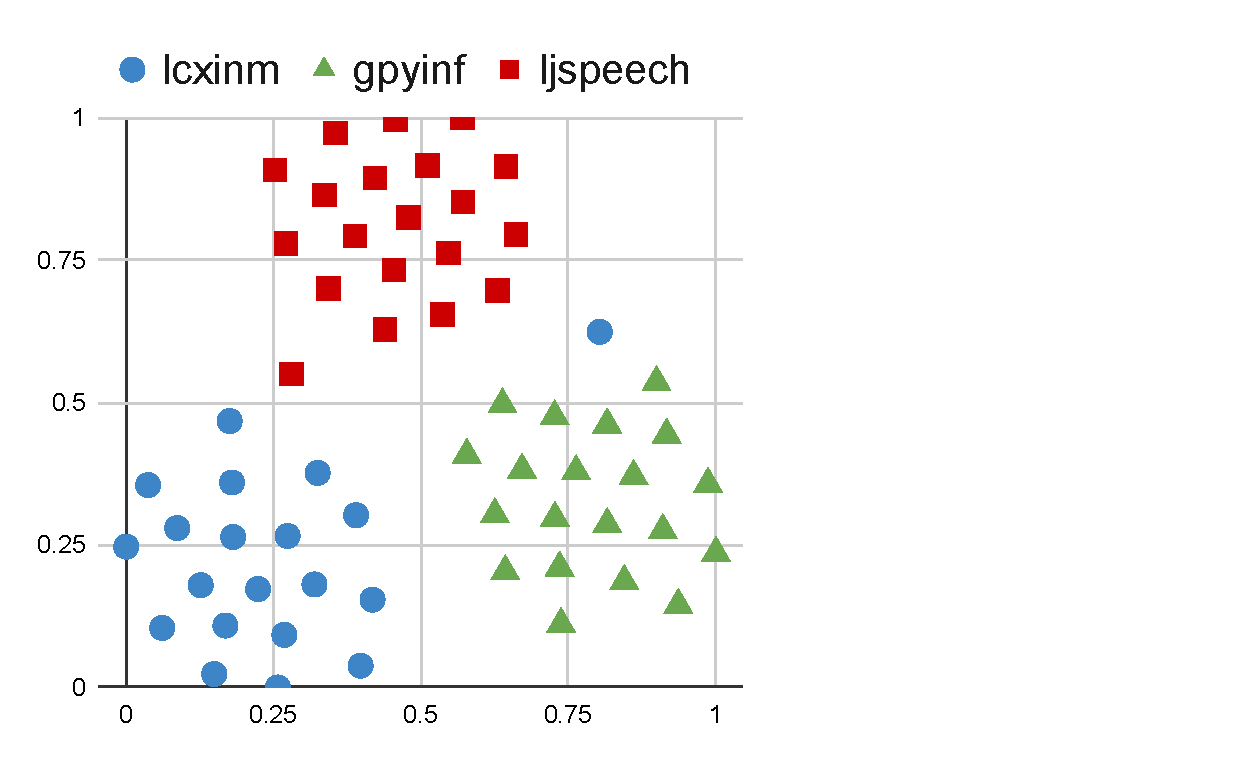
\includegraphics[width=\linewidth,trim=0 0 200 0,clip]{figure/5_dvector21.pdf}
            \caption{100 speakers w/ adv}
        \end{subfigure}        
        \begin{subfigure}[b]{0.3\linewidth}
            \centering
            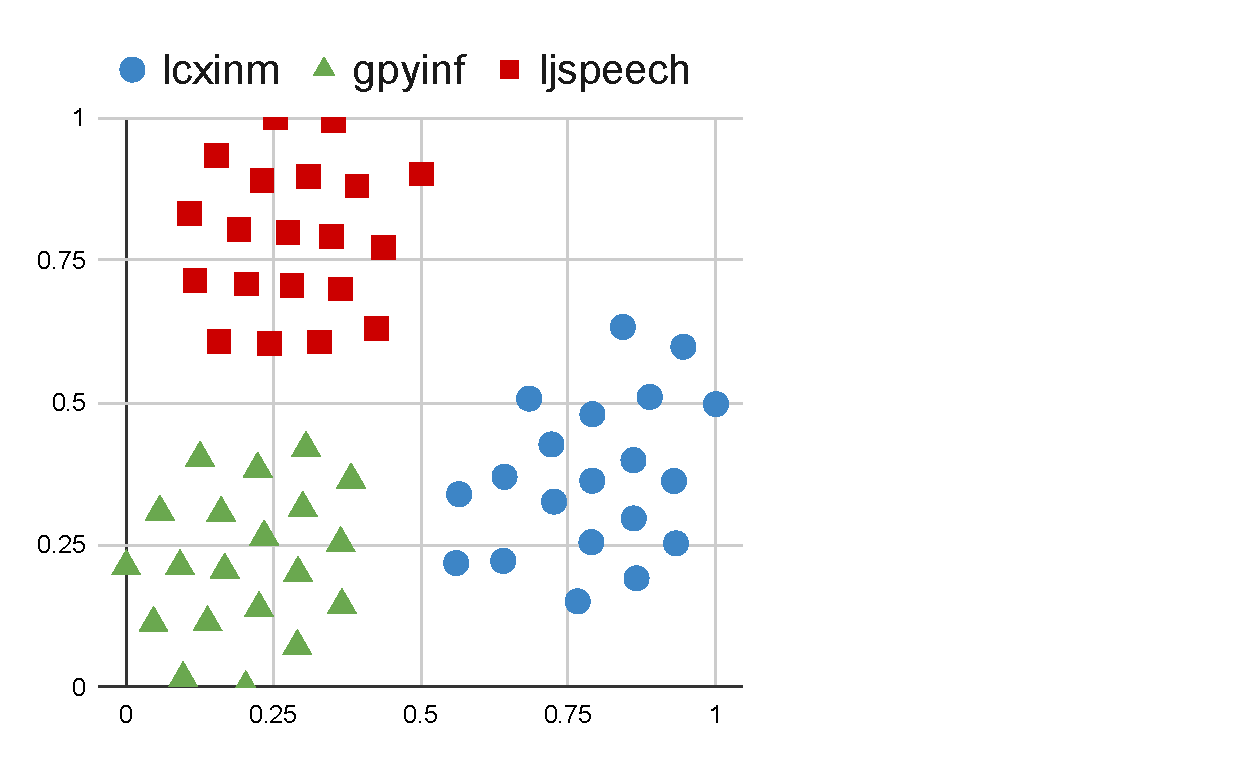
\includegraphics[width=\linewidth,trim=0 0 200 0,clip]{figure/5_dvector22.pdf}
            \caption{500 speakers w/ adv}
        \end{subfigure}   
        \begin{subfigure}[b]{0.3\linewidth}
            \centering
            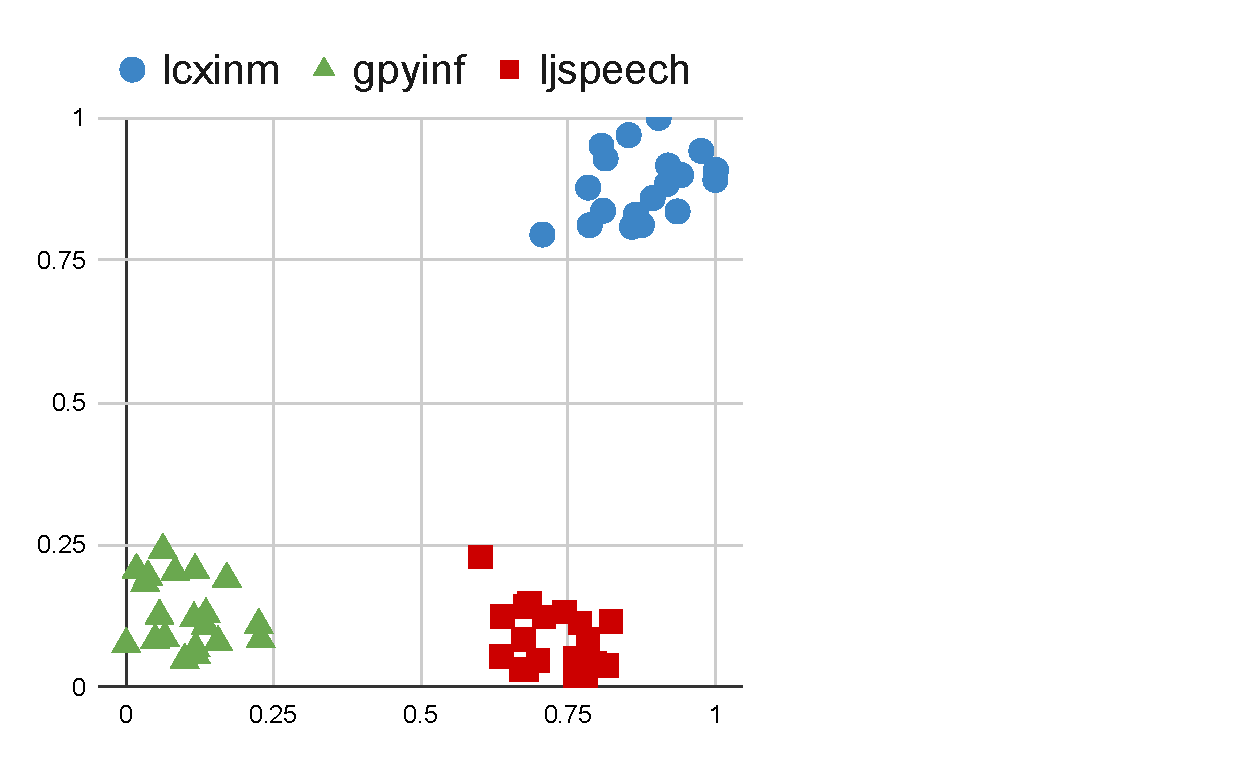
\includegraphics[width=\linewidth,trim=0 0 200 0,clip]{figure/5_dvector23.pdf}
            \caption{1000 speakers w/ adv}
        \end{subfigure}   
    \end{minipage}
    \bicaption{语音转换数据集上d-vector分布图}{Distribution of d-vector on VC corpus}
    \label{fig:dvectordis}
\end{figure}

从图~\ref{fig:dvectordis}中可以看出,即使在较少的100个说话人的训练数据集上,
也可以很好的区分三个语音转换说话人;1000个说话人训练集的模型相比100个说话人训练集和
500个说话人训练集的模型,同一类的数据更为集中,且类间距离更大,因此之后的实验将使用
1000说话人的训练集所得到的d-vector提取器模型。此外,使用语种无关对抗训练的模型
和不使用的模型在图中并无明显差异。

本章使用转换特征的d-vector与目标真实特征的d-vector之间的余弦距离来衡量转换语音相似度。
首先得到三种模型对同性别和跨性别任务的测试集转换特征,然后对每一句转换特征提取一个d-vector,
并将同一个模型的20个d-vector进行计算平均。然后将原始说话人,目标说话人和三个模型的d-vector
分别与目标说话人的d-vector计算余弦距离,计算方法为

\begin{equation}
    d_{cos} = 1-\frac{\textbf{u} \cdot \textbf{v} }{\left| \left| \textbf{u}\right| \right|_2 \left| \left| \textbf{v}\right| \right|_2}
\end{equation}

所得结果如表~\ref{tab:cosine}所示,可以看到不论是同性别还是跨性别,引入d-vector的模型所得到的说话人d-vector均好于基线模型。
但在同性别上LIDV-CycleGAN更好,反之在跨性别上DV-CycleGAN更好一些。




% 2.d-vector的差距,使用1000句的d-vector。
% 每一组:原始;目标;baseline;没有adv;有adv
\begin{table}
    \centering
    \begin{tabular}[t]{ cccccc }
        \toprule
        % \hline
        %\multirow{1}{*}{Methods} & \multicolumn{3}{|c|}{Female to male} \\
         %\cline{2-4}
        任务  & 原始 & 目标 & CycleGAN & DV-CycleGAN & LIDV-CycleGAN  \\
         %\hline
         %\hline
        \midrule
        %\hline
        同性别    &     0.3768 & 0.0 & 0.0832 & 0.0653 & \textbf{0.0422}           \\
        %\hline
        跨性别    &    0.6312 & 0.0 & 0.3099 & \textbf{0.2156} & 0.2762  \\
        \bottomrule
        \end{tabular} 
    \bicaption{转换特征和目标特征的d-vector余弦距离对比}{Comparison of cosine distance between converted and target features}
    \label{tab:cosine}
\end{table}

% cycle-consistency loss curve
% 同性别,跨性别,
% baseline, dv, lidv
% cyclea

在CycleGAN模型的训练中,重构损失是衡量模型训练好坏的一个重要标准。对于语音转换而言,如果主模型和对偶模型可以在
转换中很好的保留语义和实现说话人转换的话,重构损失则会相对较低;反之,若其中一个模型在转换中丢失了一部分语义或说话人信息,
则另一个模型会很难将其中丢失的信息恢复,导致重构损失较大。因此,本节记录了不同模型在训练过程中重构损失的变化情况。
如图~\ref{fig:re}所示。

\begin{figure}[!ht]
    \begin{minipage}[b]{\linewidth}
        \begin{subfigure}[b]{0.48\linewidth}
            \centering
            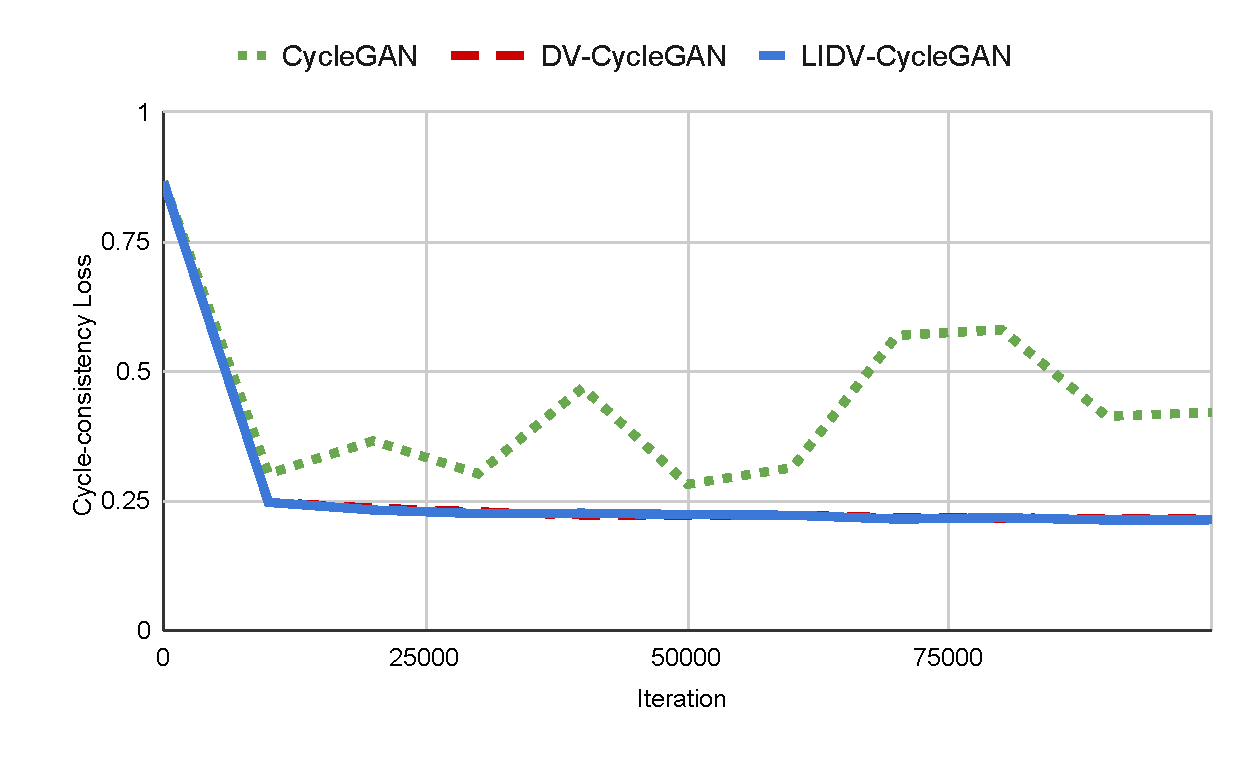
\includegraphics[width=\linewidth,trim=0 0 0 0,clip]{figure/5_cycle1.pdf}
            \caption{同性别}
        \end{subfigure}        
        \begin{subfigure}[b]{0.48\linewidth}
            \centering
            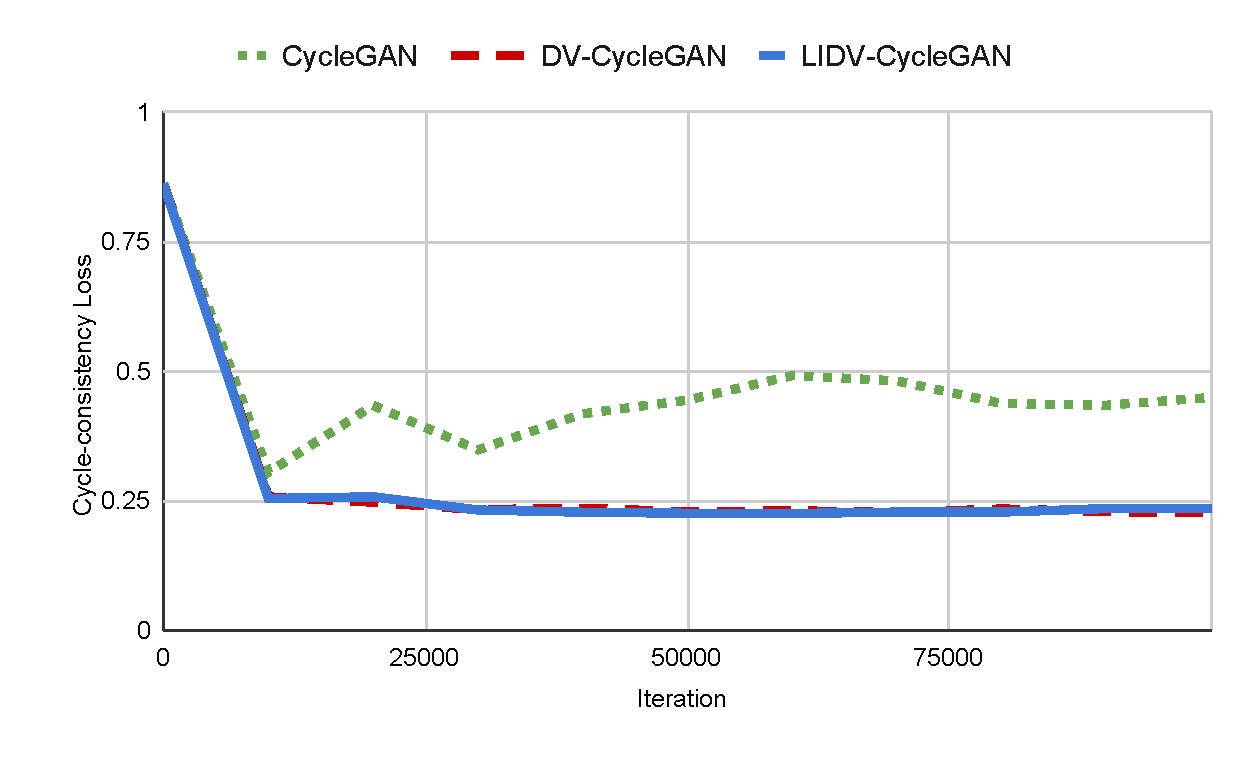
\includegraphics[width=\linewidth,trim=0 0 0 0,clip]{figure/5_cycle2.pdf}
            \caption{跨性别}
        \end{subfigure}   
    \end{minipage}
    \bicaption{训练阶段重构损失变化曲线}{Line graph of the reconstruct loss during training phase}
    \label{fig:re}
\end{figure}

图中绿色点线为基线模型,红色虚线为引入d-vector没有加入语种无关训练的模型,蓝色实线为引入d-vector且加入语种无关训练的模型。
在两个图中,基线模型的重构损失在训练过程中损失值较高,且较不稳定。而另外两个模型的重构损失曲线则一直处于较为稳定的状态。在这里,
是否使用语种无关的方法也并没有显著区别,该论点将在主观试验中进一步验证。这里需要说明的是,对于基线模型来说,在训练的一开始,即
第10000步的时候损失较低,而随后的训练则会通常高于该损失值。这是因为在训练开始的前10000步时,模型训练使用了身份损失,该损失
在训练初始阶段可以较好的保留语义,但也会保留说话人信息,因此通常只会用于模型训练的初始阶段。当该损失在之后的训练去掉后,
基线模型就没有了语义的约束,如前文所述,此时特征中的语义信息会影响判别器的判断,当语义信息差别较大时,判别器可能会变成语种分类器。
此时判别器对生成器回传的梯度会改变生成器转换特征中的语义信息,当语义信息改变时,对偶模型的重构难度会加大,从而导致重构损失的上升。
在基线模型的转换语音中,基本上无法听出合理的语义,这在之后的主观实验中也可以看到这一点。
作者也尝试过增加身份损失的训练时间,或者增加其损失权重,但是这个无法解决模型本身的弊端。
在以往的试验中,只要身份损失存在,语义就可以较好的保留,同时说话人也更难转换,
但只要身份损失去掉,语义信息就会大量丢失。

\subsection{主观实验}
在主观实验中,针对语音自然度的测试选择使用主观意见分(MOS)测试,对语音的相似度则使用偏好测试(ABX),且两个主观测试都在同性别
和跨性别任务上进行测试。在MOS测试中,每一位测试人员需要做多组音频对比,其中每一组音频中包括目标真实音频,基线转换音频,DV-CycleGAN
转换音频和LIDV-CycleGAN转换音频。测试人员需要逐个听并对每个音频进行打分,分值从1到5,每一组的第一个音频都是目标真实音频,表示
5分的参考,剩下的三组音频随机打乱。每组实验包括不少于6名测试人员参与。测试人员打分的标准主要是判断语音是否自然,发音是否清晰,是否有噪音等。
其中1分表示完全不自然(非常不像人类说的话,且完全无法分辨发音);2分表示不自然(不像人类说的话,但能基本分辨每个发音, 但噪音较大);
3分表示稍不自然(较像一个人说的话,但有个别音调错误或发音含糊不清, 有噪音);
4分表示自然(像一个人说的话,发音清晰,没有音调错误,基本没有噪音);5分表示非常自然(非常像一个人说的话,发音清晰, 没有噪音)。
在偏好测试中,每一组包括三个音频,第一个音频是目标音频,剩下两个为对照组音频,测试者首先需要听目标音频,然后再听顺序打乱的对照音频,并选择哪个音频
更像目标说话人说的,即相似度的判断。有三个选项可以选择:更偏好第一个,更偏好第二个,以及没有偏好。偏好测试分为两组,一组为基线模型(Baseline)和
LIDV-CycleGAN模型的偏好对比,另一组为DV-CycleGAN和LIDV-CycleGAN的偏好对比。所有测试皆在安静,测试人员
戴耳机的条件下进行。

图~\ref{fig:mos2}展示了MOS测试的结果。其中最左列为满分5分的真实音频。可以看到,基线模型的转换音频都没有达到2分,这是因为基线模型
不仅转换了说话人,也对语义信息进行了转换,直观的感受是尽管输入是英文语音,但转换出来的语音缺听起来像中文,同事转换语音的语义信息丢失非常严重,
测试人员普遍无法判别所说语音的内容,从而导致MOS打分的下降。同时,使用本章提出的引入说话人特征的模型分数均
高于基线模型,由于跨性别任务本身难度较大于同性别任务,因此同性别任务上的提升更为明显。在同性别和跨性别试验中,LIDV-CycleGAN模型都要略好于DV-CycleGAN模型,
这也在一定程度上验证了说话人无关特征提取器的有效性。除此之外,在图中可以看到转换音质的打分均没有超过
3分,主要原因是由于本文使用了GL声码器,该声码器的好处是可以完整还原特征对应的音频,但是合成音质相比传统的数字信号声码器和神经网络声码器都要
较差一些,主要特征是合成语音频谱信息较少,且存在明显的相位问题,这些都会影响主观测评的分数。

\begin{figure}[!ht]
    \begin{minipage}[b]{\linewidth}
        \begin{subfigure}[b]{0.48\linewidth}
            \centering
            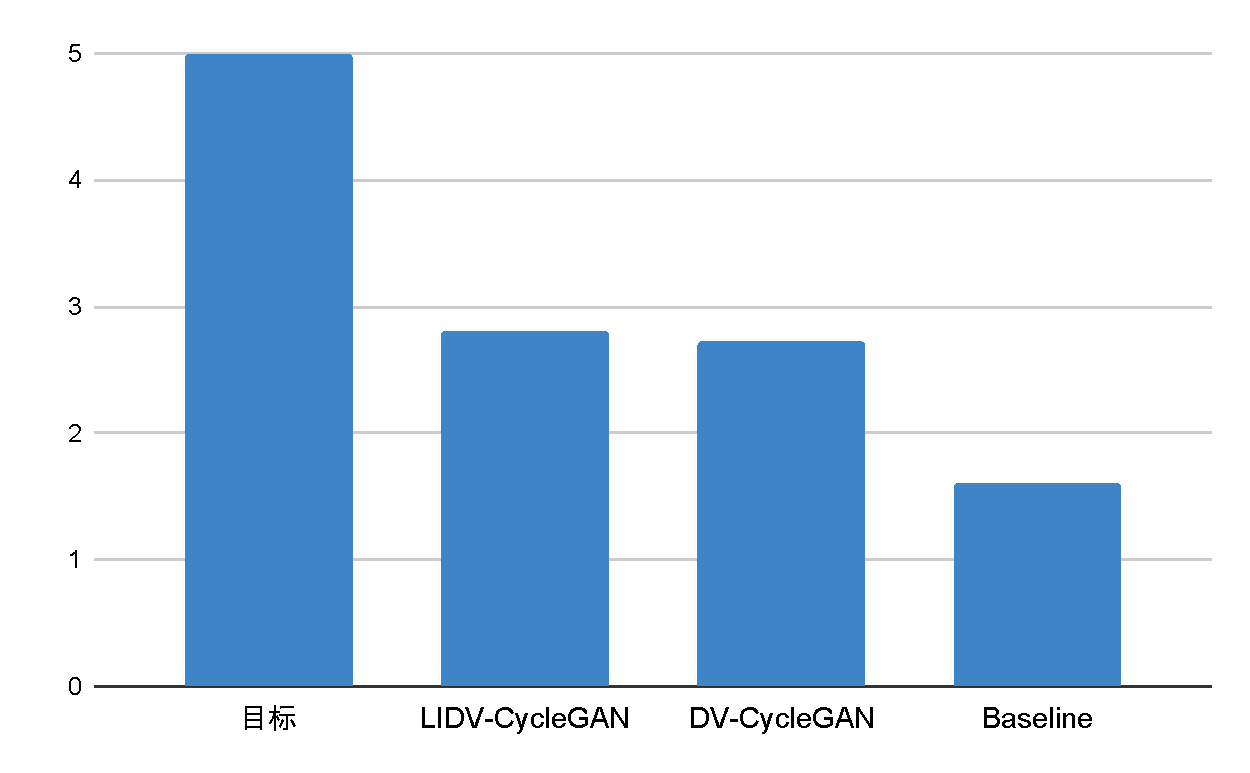
\includegraphics[width=\linewidth,trim=0 0 0 0,clip]{figure/5_mosintra.pdf}
            \caption{同性别}
        \end{subfigure}        
        \begin{subfigure}[b]{0.48\linewidth}
            \centering
            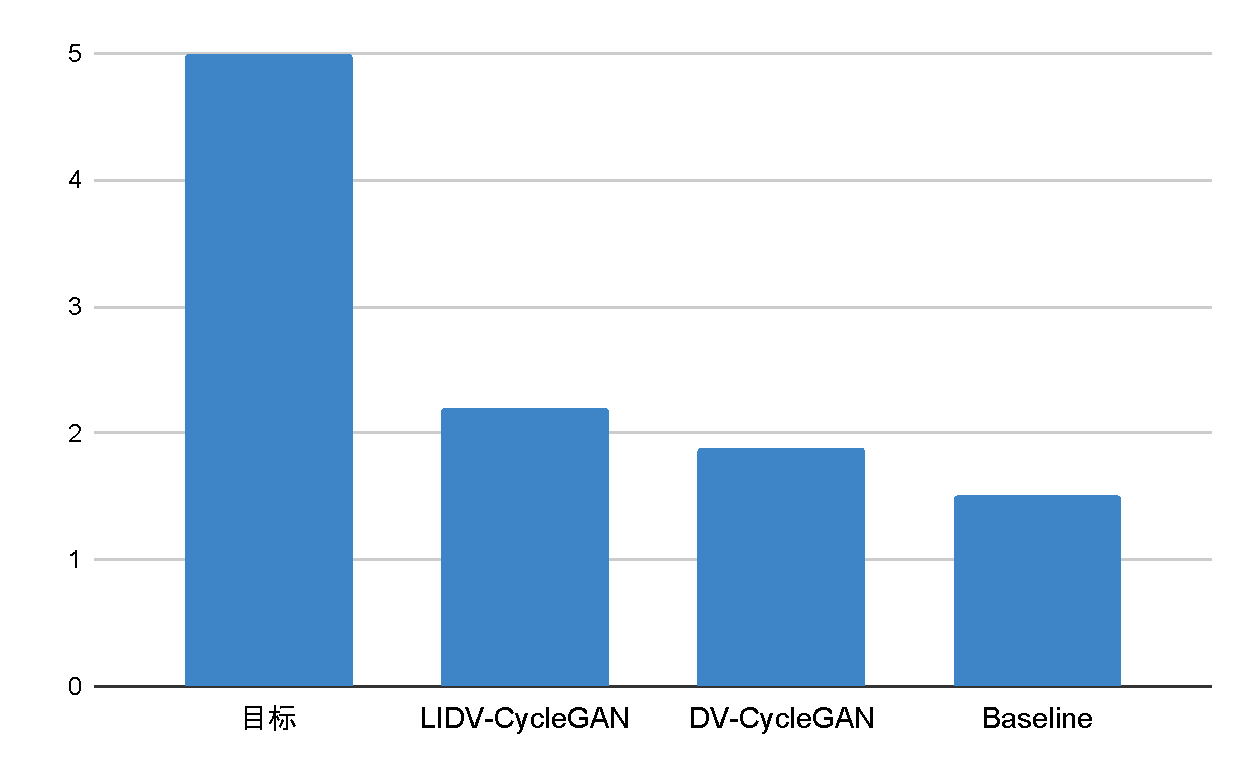
\includegraphics[width=\linewidth,trim=0 0 0 0,clip]{figure/5_mosinter.pdf}
            \caption{跨性别}
        \end{subfigure}   
    \end{minipage}
    \bicaption{MOS主观测评对比图}{Comparison of the MOS test result}
    \label{fig:mos2}
\end{figure}

表~\ref{tab:simtable}展示了相似度偏好测试的结果。在上面两组试验中,可以看出使用说话人特征的LIDV-CycleGAN模型在相似度上好于基线模型,
由于在跨性别上基线模型的转换语音噪音太大,语义丢失严重,基本为不可用的转换模型,因此在相似度偏好上都和所提方法有着较大的差距。
在使用语种无关的说话人特征提取器(DV-CycleGAN和LIDV-CycleGAN)的试验中,使用了语种无关的对抗方法的模型略好于没有使用的模型,
但考虑到大部分测试人员仍选择了无偏好,因此两个模型在相似度上相差都不明显。如前文所述,语种无关的说话人特征提取器所提取的特征
与真实目标特征的误差相比没有使用语种无关训练方法的模型相差并不大。因此两者在相似度上也不会出现明显的差别。

\begin{table}
    \centering
    \bicaption{转换模型的相似度偏好测试(\%)}{The result of ABX test of different methods}
    \begin{tabular}[t]{ ccc }
        \toprule
        % \hline
        %\multirow{1}{*}{Methods} & \multicolumn{3}{|c|}{Female to male} \\
         %\cline{2-4}
        模型  & 同性别 & 跨性别   \\
         %\hline
         %\hline
        \midrule
        %\hline
        baseline    & 10 & 0.0           \\
        LIDV-CycleGAN    & 62.5 & 50           \\
        无偏好    & 27.5 & 50           \\
        %\hline
        \midrule
        DV-CycleGAN    & 8.33 & 0.0           \\
        LIDV-CycleGAN    & 16.67 & 12.5           \\
        无偏好 & 75 & 87.5           \\
        \bottomrule
        \end{tabular} 
    \label{tab:simtable}
\end{table}

\section{本章小结}
对于跨语种语音转换任务,本章在CycleGAN语音转换方法下提出了基于说话人特征d-vector的语音转换方法。该方法
用说话人识别语料预训练一个说话人分类模型。将该模型的输出层去掉,则得到了说话人特征提取器。该提取器作为一个
不可训练,但是可以前向计算和反向传播的说话人信息过滤器,与判别器结合在一起。使得判别器在判别正负例的时候可以
只考虑说话人信息,帮助生成器实现更好的转换。实验证明基于说话人特征的CycleGAN模型可以有效提升跨语种语音转换
的自然度和相似度,同时对于说话人特征提取器而言,使用语种无关的对抗训练方式可以略微提升转换效果。
但是该方法的转换音频仍旧有较大的提升空间,一方面转换特征的语义虽然可以较好的保留,但是其自然度仍旧较差,且有较多的噪音,尤其在跨性别任务上;另一方面,目前使用的是GL声码器,GL声码器
在音频自然度上有天生的缺陷,但是若要使用神经网络声码器如WaveNet,则又需要考虑双语合成的问题,这也是未来的一个
重要研究方向。


\backmatter
\chapter{全文总结}
非平行语料语音转换是语音转换中非常重要的一个方向。本文工作主要基于CycleGAN语音转换方法,
围绕不同的非平行语料语音转换任务展开。

首先对于标准的非平行语料语音转换任务,
本文提出半优化循环一致性生成对抗网络(Semi-optimized CycleGAN)和基频辅助特征的高音质非平行语料语音转换系统。
该系统使用梅尔频谱作为声学特征,WaveNet模型作为声码器。经过分析,本文对标准CycleGAN模型的
训练过程进行改进,去除了其中影响生成器训练的更新过程,使得生成器在每个周期中只有其中一个被优化;
同时针对转换中音调错误的问题,提出使用基频辅助特征来提升生成器对基频的隐式表达能力。实验表明,
半优化CycleGAN不但可以显著地减小模型训练过程中在测试集上的梅尔频谱距离,也可以减小转换基频与
目标基频之间的误差。在自然度和相似度的主观实验中,半优化CycleGAN和基频辅助特征都对转换语音有着较好的提升。
尤其在男性转男性的任务上,发音错误问题较为严重,基频辅助特征使其MOS分数有了明显的提升。实验也比较了
不同大小训练数据量对模型性能的影响,发现在训练集在最少为500句话的时候都可以得到较高的音质。

对于难度更高的跨语种语音转换任务,本文提出了基于说话人特征的语音转换模型。首先用说话人识别的
语料训练一个说话人识别模型,然后将说话人识别模型的最后一层去掉得到说话人特征提取器。将该提取器
与CycleGAN模型进行结合,其作为判别器的前置网络,从输入的声学特征中提取说话人信息,来减少
语义信息对判别器的影响,从而提升转换效果。实验表明,对于语音转换的较少说话人而言,100个说话人
的训练集得到的说话人特征提取器也可以对语音转换说话人进行较好的分离。同时,说话人特征的引入不但可以
减小转换音频说话人特征与真实音频说话人特征之间的余弦距离,还可以使得模型训练中重构损失更稳定。
在主观测试中,引入说话人特征的方法在自然度和相似度上都要好于没有引入说话人特征的标准CycleGAN模型,
另一方面,使用语种无关的对抗训练方法而得到的语种无关的说话人提取器,可以略微提升转换语音的自然度和相似度。
但是,当前方法与真实语音在自然度和相似度上都还有不小的差距,一方面是由于生成语音的噪声较大,尽管语义相比
基线模型有所提升,但依旧不够清晰,与语种内语音转换仍有较大差距,转换模型仍有很大的提升空间;另一方面,声码器也是制约音质的一个因素,
将目前使用的跨语种语音转换方法应用到神经网络声码器中也是未来的重点研究方向。

% 使用英文字母对附录编号
\appendix

% 附录内容,本科学位论文可以用翻译的文献替代。
%% !TEX root = ../thesis.tex

\chapter{Maxwell Equations}

选择二维情况,有如下的偏振矢量:
\begin{subequations}
  \begin{align}
    {\bf E} &= E_z(r, \theta) \hat{\bf z} \\
    {\bf H} &= H_r(r, \theta) \hat{\bf r} + H_\theta(r, \theta) \hat{\bm\theta}
  \end{align}
\end{subequations}
对上式求旋度:
\begin{subequations}
  \begin{align}
    \nabla \times {\bf E} &= \frac{1}{r} \frac{\partial E_z}{\partial\theta}
      \hat{\bf r} - \frac{\partial E_z}{\partial r} \hat{\bm\theta} \\
    \nabla \times {\bf H} &= \left[\frac{1}{r} \frac{\partial}{\partial r}
      (r H_\theta) - \frac{1}{r} \frac{\partial H_r}{\partial\theta} \right]
      \hat{\bf z}
  \end{align}
\end{subequations}
因为在柱坐标系下,$\overline{\overline\mu}$ 是对角的,所以 Maxwell 方程组中电场
$\bf E$ 的旋度:
\begin{subequations}
  \begin{align}
    & \nabla \times {\bf E} = \upi \omega {\bf B} \\
    & \frac{1}{r} \frac{\partial E_z}{\partial\theta} \hat{\bf r} -
      \frac{\partial E_z}{\partial r}\hat{\bm\theta} = \upi \omega \mu_r H_r
      \hat{\bf r} + \upi \omega \mu_\theta H_\theta \hat{\bm\theta}
  \end{align}
\end{subequations}
所以 $\bf H$ 的各个分量可以写为:
\begin{subequations}
  \begin{align}
    H_r &= \frac{1}{\upi \omega \mu_r} \frac{1}{r}
      \frac{\partial E_z}{\partial\theta} \\
    H_\theta &= -\frac{1}{\upi \omega \mu_\theta}
      \frac{\partial E_z}{\partial r}
  \end{align}
\end{subequations}
同样地,在柱坐标系下,$\overline{\overline\epsilon}$ 是对角的,所以 Maxwell 方程
组中磁场 $\bf H$ 的旋度:
\begin{subequations}
  \begin{align}
    & \nabla \times {\bf H} = -\upi \omega {\bf D} \\
    & \left[\frac{1}{r} \frac{\partial}{\partial r}(r H_\theta) - \frac{1}{r}
      \frac{\partial H_r}{\partial\theta} \right] \hat{\bf z} = -\upi \omega
      {\overline{\overline\epsilon}} {\bf E} = -\upi \omega \epsilon_z E_z
      \hat{\bf z} \\
    & \frac{1}{r} \frac{\partial}{\partial r}(r H_\theta) - \frac{1}{r}
      \frac{\partial H_r}{\partial\theta} = -\upi \omega \epsilon_z E_z
  \end{align}
\end{subequations}
由此我们可以得到关于 $E_z$ 的波函数方程:
\begin{equation}
  \frac{1}{\mu_\theta \epsilon_z} \frac{1}{r} \frac{\partial}{\partial r}
  \left(r \frac{\partial E_z}{\partial r} \right) + \frac{1}{\mu_r \epsilon_z}
  \frac{1}{r^2} \frac{\partial^2E_z}{\partial\theta^2} +\omega^2 E_z = 0
\end{equation}

%% !TEX root = ../thesis.tex

\chapter{绘制流程图}

图~\ref{fig:flow_chart} 是一张流程图示意。使用 \pkg{tikz} 环境,搭配四种预定义节
点(\verb+startstop+、\verb+process+、\verb+decision+和\verb+io+),可以容易地绘
制出流程图。

\begin{figure}[!htp]
  \centering
  \resizebox{6cm}{!}{\begin{tikzpicture}[node distance=2cm]
    \node (pic) [startstop] {待测图片};
    \node (bg) [io, below of=pic] {读取背景};
    \node (pair) [process, below of=bg] {匹配特征点对};
    \node (threshold) [decision, below of=pair, yshift=-0.5cm] {多于阈值};
    \node (clear) [decision, right of=threshold, xshift=3cm] {清晰?};
    \node (capture) [process, right of=pair, xshift=3cm, yshift=0.5cm] {重采};
    \node (matrix_p) [process, below of=threshold, yshift=-0.8cm] {透视变换矩阵};
    \node (matrix_a) [process, right of=matrix_p, xshift=3cm] {仿射变换矩阵};
    \node (reg) [process, below of=matrix_p] {图像修正};
    \node (return) [startstop, below of=reg] {配准结果};
     
    %连接具体形状
    \draw [arrow](pic) -- (bg);
    \draw [arrow](bg) -- (pair);
    \draw [arrow](pair) -- (threshold);

    \draw [arrow](threshold) -- node[anchor=south] {否} (clear);

    \draw [arrow](clear) -- node[anchor=west] {否} (capture);
    \draw [arrow](capture) |- (pic);
    \draw [arrow](clear) -- node[anchor=west] {是} (matrix_a);
    \draw [arrow](matrix_a) |- (reg);

    \draw [arrow](threshold) -- node[anchor=east] {是} (matrix_p);
    \draw [arrow](matrix_p) -- (reg);
    \draw [arrow](reg) -- (return);
\end{tikzpicture}
}
  \bicaption{绘制流程图效果}{Flow chart}
  \label{fig:flow_chart}
\end{figure}


% 文后无编号部分
\backmatter




% 参考资料
\printbibliography[heading=bibintoc]

% 用于盲审的论文需隐去致谢、发表论文、参与项目、申请专利、简历

% 致谢
% !TEX root = ../thesis.tex

%TC:ignore

\begin{acknowledgements}
  感谢那位最先制作出博士学位论文 \LaTeX 模板的交大物理系同学!

  感谢 William Wang 同学对模板移植做出的巨大贡献!

  感谢 \href{https://github.com/weijianwen}{@weijianwen} 学长一直以来的开发和维
  护工作!

  感谢 \href{https://github.com/sjtug}{@sjtug} 以及
   \href{https://github.com/dyweb}{@dyweb} 对 0.9.5 之后版本的开发和维护工作!

  感谢所有为模板贡献过代码的同学们, 以及所有测试和使用模板的各位同学!

  感谢 \LaTeX 和 \href{https://github.com/sjtug/SJTUThesis}{\sjtuthesis},帮我节
  省了不少时间。
\end{acknowledgements}

%TC:endignore


% 发表论文、参与项目、申请专利、简历
% 盲审论文中,发表学术论文及参与科研情况等仅以第几作者注明即可,不要出现作者或他人姓名
%% !TEX root = ../thesis.tex

%TC:ignore

\begin{publications}
  \item Chen H, Chan C~T. Acoustic cloaking in three dimensions using acoustic metamaterials[J]. Applied Physics Letters, 2007, 91:183518.
  \item Chen H, Wu B~I, Zhang B, et al. Electromagnetic Wave Interactions with a Metamaterial Cloak[J]. Physical Review Letters, 2007, 99(6):63903.
\end{publications}

\begin{publications*}
  \item 第一作者. 中文核心期刊论文, 2007.
  \item 第一作者. EI 国际会议论文, 2006.
\end{publications*}

%TC:endignore

%% !TEX root = ../thesis.tex

%TC:ignore

\begin{projects}
  \item 参与973项目子课题(2007年6月--2008年5月)
  \item 参与自然基金项目(2005年5月--2005年8月)
  \item 参与国防项目(2005年8月--2005年10月)
\end{projects}

\begin{projects*}
  \item 973项目“XXX”
  \item 自然基金项目“XXX”
  \item 国防项目“XXX”
\end{projects*}

%TC:endignore

% !TEX root = ../thesis.tex

%TC:ignore

\begin{patents}
  \item 第一发明人,“采样半优化CycleGAN模型的语音转换方法和装置”,专利申请号201910515510.5
  \item 第一发明人,“儿童语音识别模型的训练方法及系统”,专利申请号201911000370.4
\end{patents}

\begin{patents*}
  \item 第一发明人,“采样半优化CycleGAN模型的语音转换方法和装置”,专利申请号201910515510.5
  \item 第一发明人,“儿童语音识别模型的训练方法及系统”,专利申请号201911000370.4
\end{patents*}

%TC:endignore

%% !TEX root = ../thesis.tex

%TC:ignore

\begin{resume}
  \subsection*{基本情况}
    某某,yyyy 年 mm 月生于 xxxx。

  \subsection*{教育背景}
  \begin{itemize}
    \item yyyy 年 mm 月至今,上海交通大学,博士研究生,xx 专业
    \item yyyy 年 mm 月至 yyyy 年 mm 月,上海交通大学,硕士研究生,xx 专业
    \item yyyy 年 mm 月至 yyyy 年 mm 月,上海交通大学,本科,xx 专业
  \end{itemize}

  \subsection*{研究兴趣}
    \LaTeX{} 排版

  \subsection*{联系方式}
  \begin{itemize}
    \item 地址: 上海市闵行区东川路 800 号,200240
    \item E-mail: \email{xxx@sjtu.edu.cn}
  \end{itemize}
\end{resume}

%TC:endignore


% 中文学士学位论文要求在最后有一个英文大摘要,单独编页码,英文学士学位论文不需要
% !TEX root = ../thesis.tex

\begin{bigabstract}
  An imperial edict issued in 1896 by Emperor Guangxu, established Nanyang
  Public School in Shanghai. The normal school, school of foreign studies,
  middle school and a high school were established. Sheng Xuanhuai, the person
  responsible for proposing the idea to the emperor, became the first president
  and is regarded as the founder of the university.

  During the 1930s, the university gained a reputation of nurturing top
  engineers. After the foundation of People's Republic, some faculties were
  transferred to other universities. A significant amount of its faculty were
  sent in 1956, by the national government, to Xi'an to help build up Xi'an Jiao
  Tong University in western China. Afterwards, the school was officially
  renamed Shanghai Jiao Tong University.

  Since the reform and opening up policy in China, SJTU has taken the lead in
  management reform of institutions for higher education, regaining its vigor
  and vitality with an unprecedented momentum of growth. SJTU includes five
  beautiful campuses, Xuhui, Minhang, Luwan Qibao, and Fahua, taking up an area
  of about 3,225,833 m2. A number of disciplines have been advancing towards the
  top echelon internationally, and a batch of burgeoning branches of learning
  have taken an important position domestically.

  Today SJTU has 31 schools (departments), 63 undergraduate programs, 250
  masters-degree programs, 203 Ph.D. programs, 28 post-doctorate programs, and
  11 state key laboratories and national engineering research centers.

  SJTU boasts a large number of famous scientists and professors, including 35
  academics of the Academy of Sciences and Academy of Engineering, 95 accredited
  professors and chair professors of the "Cheung Kong Scholars Program" and more
  than 2,000 professors and associate professors.

  Its total enrollment of students amounts to 35,929, of which 1,564 are
  international students. There are 16,802 undergraduates, and 17,563 masters
  and Ph.D. candidates. After more than a century of operation, Jiao Tong
  University has inherited the old tradition of "high starting points, solid
  foundation, strict requirements and extensive practice." Students from SJTU
  have won top prizes in various competitions, including ACM International
  Collegiate Programming Contest, International Mathematical Contest in Modeling
  and Electronics Design Contests. Famous alumni include Jiang Zemin, Lu Dingyi,
  Ding Guangen, Wang Daohan, Qian Xuesen, Wu Wenjun, Zou Taofen, Mao Yisheng,
  Cai Er, Huang Yanpei, Shao Lizi, Wang An and many more. More than 200 of the
  academics of the Chinese Academy of Sciences and Chinese Academy of
  Engineering are alumni of Jiao Tong University.
\end{bigabstract}


\end{document}
